\documentclass{article}
\usepackage[legalpaper, margin=1.2in]{geometry}
\usepackage{graphicx}
\usepackage{caption}
\usepackage{amsfonts}
\usepackage{mathptmx}
\usepackage{subcaption}
\usepackage{hyperref}
\hypersetup{
    colorlinks=true,
    linkcolor=blue,
    filecolor=blue,      
    urlcolor=blue,
    citecolor=blue,
}


\title{Artificial Neural Networks and Deep Learning: Report}
\author{Feiyang Tang (r0728168)\\
Master of Artificial Intelligence (Track: BDA)}
\date{}

\begin{document}

\maketitle

\section{Supervised learning and generalisation}
In this section, we focused on feed-forward Neural Networks. There are two exercises in this section.

\subsection{Comparison of algorithms}
For this exercise, we are going to perform comparison of various algorithms against \textit{Gradient Descent} (\verb|traingd|) such as \textit{Levenberg Marquardt} (\verb|trainlm|), \textit{BFGS Quasi-Newton} (\verb|trainbfg|), \textit{Fletcher-Reeves conjugate gradient} (\verb|traincgf|) and \textit{Polak-Ribiere conjugate gradient} (\verb|traincgp|).

Many parameters could potentially affect the performance of neural networks, for example, numbers of hidden neurons, numbers of training sets, the level of noise and the design of training functions, etc. The training function algorithms listed above will be evaluated.

Regarding the evaluation of neural networks, we mostly use Mean Squared Error (MSE) as the primary metric (correctness) along with the running time (speed) and in some cases, the situation of over-fitting (when noises are added). While in most cases a high R-value indicates a good fit, this cannot be guaranteed. We shall also look at the residuals, which should be random noise - must not show any visible pattern. 

\subsubsection{Function approximation comparison without noises}
The function to estimate is $y=\sin \left(x^{2}\right)$ with points $x=0: 0.05: 3 \pi$.

Figure \ref{linear1} gives us a general idea on how \verb|trainlm| and \verb|traingd| work on our sine function. It is easy to notice that \verb|trainlm| fits the actual function much better, also comes with a higher R-value: 1. Figure \ref{fig:lmgdapprox} also illustrates the approximation curves of both the training algorithm and the actual targets. It is clear that \verb|trainlm| can perfectly match the target with approximations while \verb|traingd| cannot achieve a satisfactory goal.

\begin{figure}[h!]
  \centering
  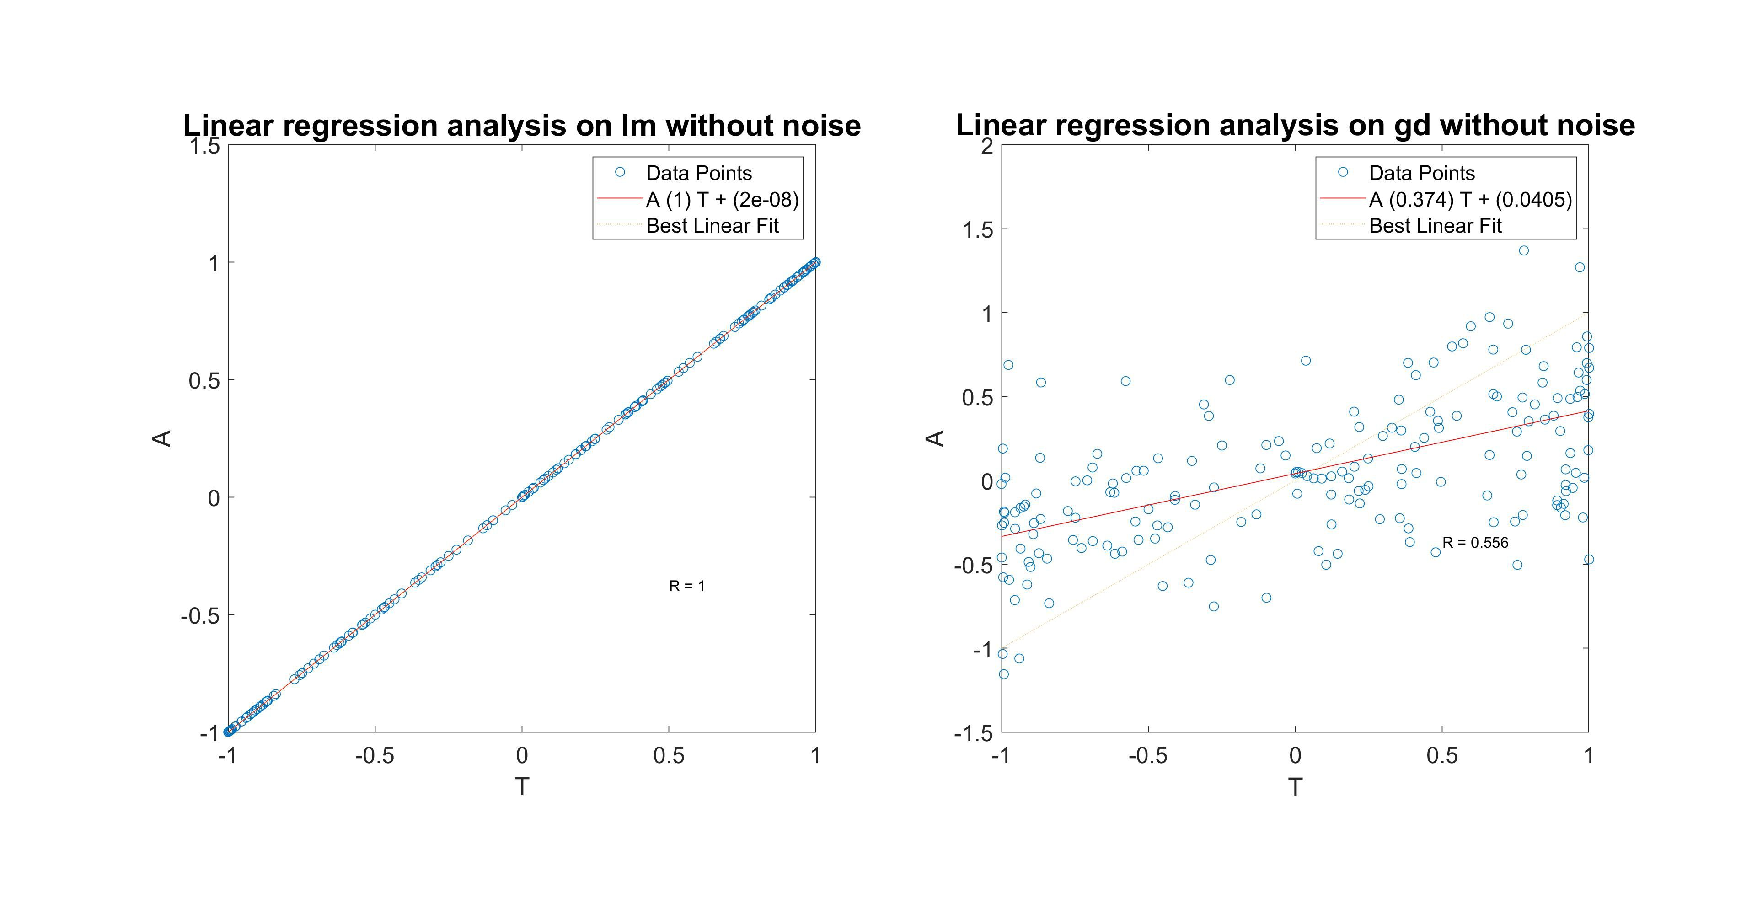
\includegraphics[width=\textwidth]{lab1/lmgdcomparewithoutnoise.pdf}
  \caption{Linear regression analysis on GD and LM}
  \label{linear1}
\end{figure}

\begin{figure}[h!]
  \centering
  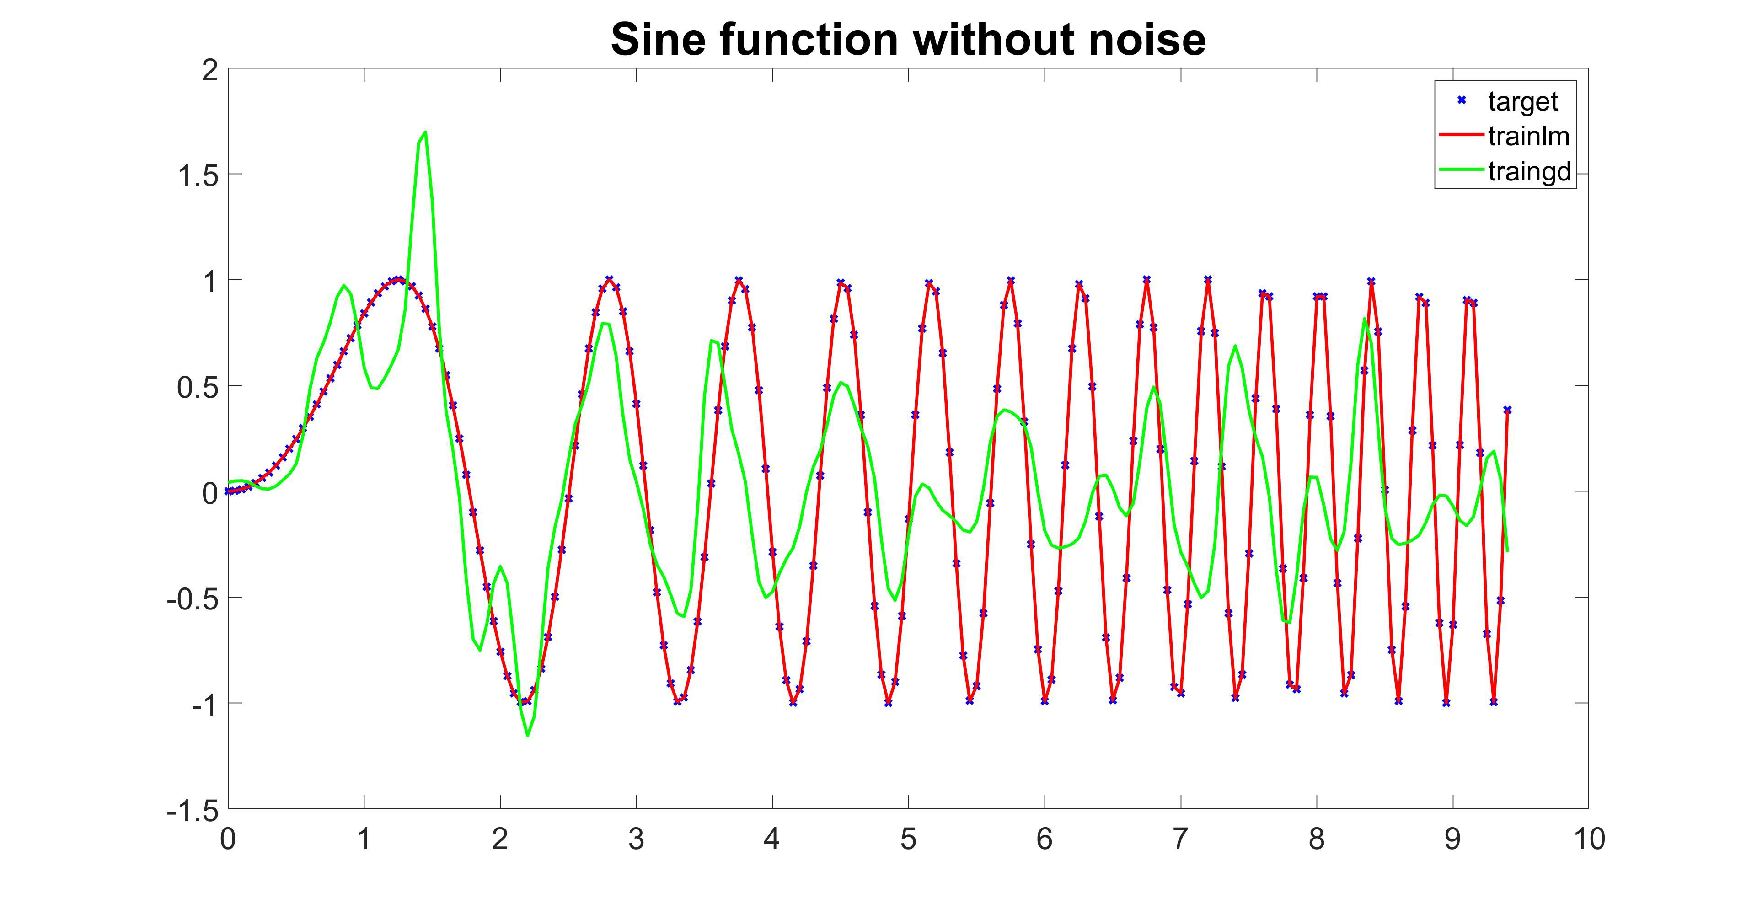
\includegraphics[width=.9\textwidth]{lab1/sinenonoise.pdf}
  \caption{Sine function approximation result on GD and LM}
  \label{fig:lmgdapprox}
\end{figure}


\begin{figure}[h!]
  \centering
  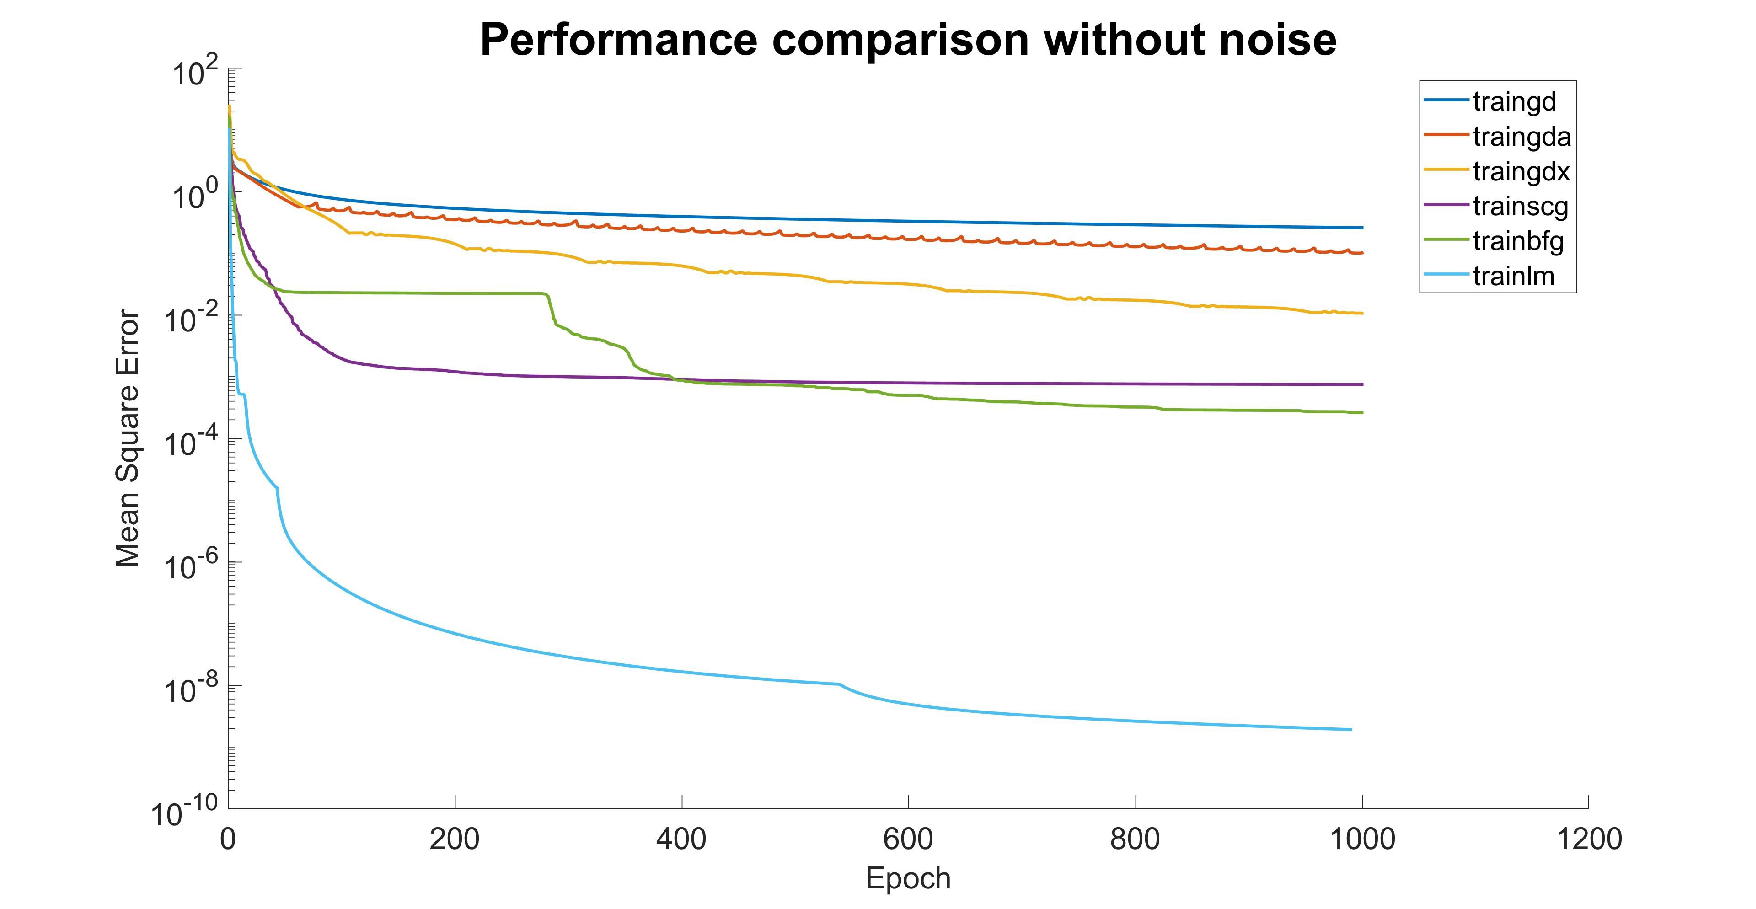
\includegraphics[width=.9\textwidth]{lab1/performancenonoise.pdf}
  \caption{Various algorithm performance comparison on Sine function}
  \label{fig:compare1}
\end{figure}

How about the other algorithms we mentioned before? Figure \ref{fig:compare1} provides a comparison among six training algorithms on their performance of sine function approximation. It was evident that \verb|trainlm| surpasses almost every other algorithms in this case on achieving the least MSE.

%%%%%%%%%%%5
%\begin{figure}[h!]
%\begin{subfigure}[b]{.49\textwidth}
%  \centering
  % include first image
%  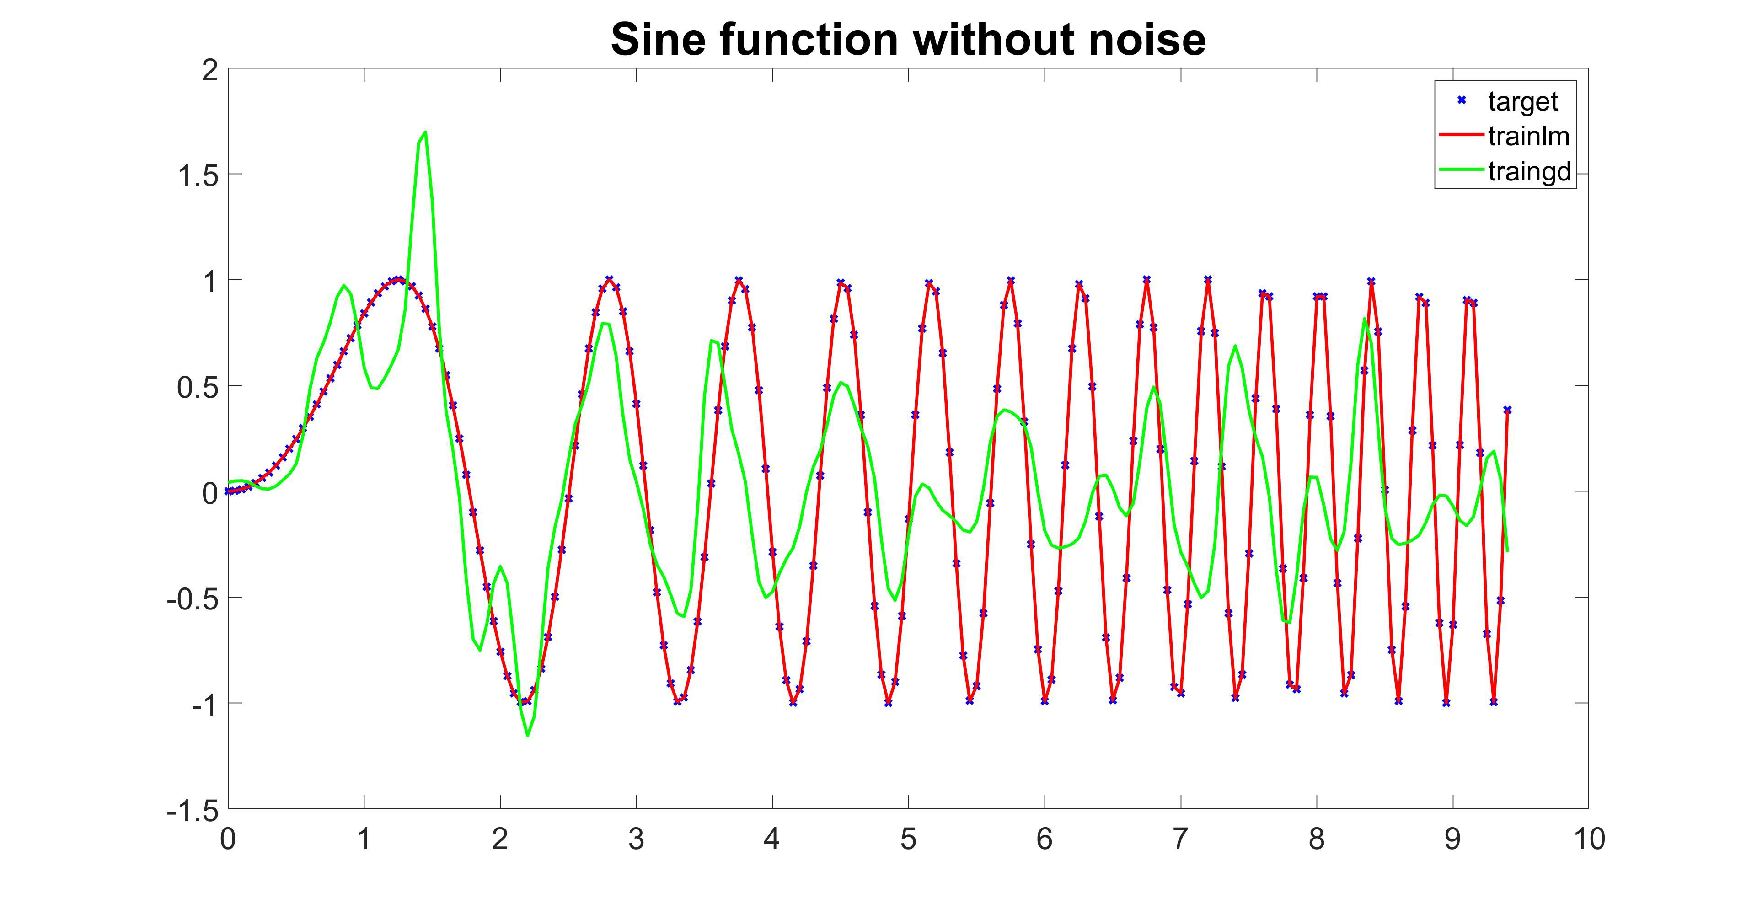
\includegraphics[width=\linewidth]{lab1/sinenonoise.pdf}
%  \caption{Sine function approximation result on GD and LM}
%  \label{fig:lmgdapprox}
%\end{subfigure}
%\hfill
%\begin{subfigure}[b]{.49\textwidth}
%  \centering
  % include second image
%  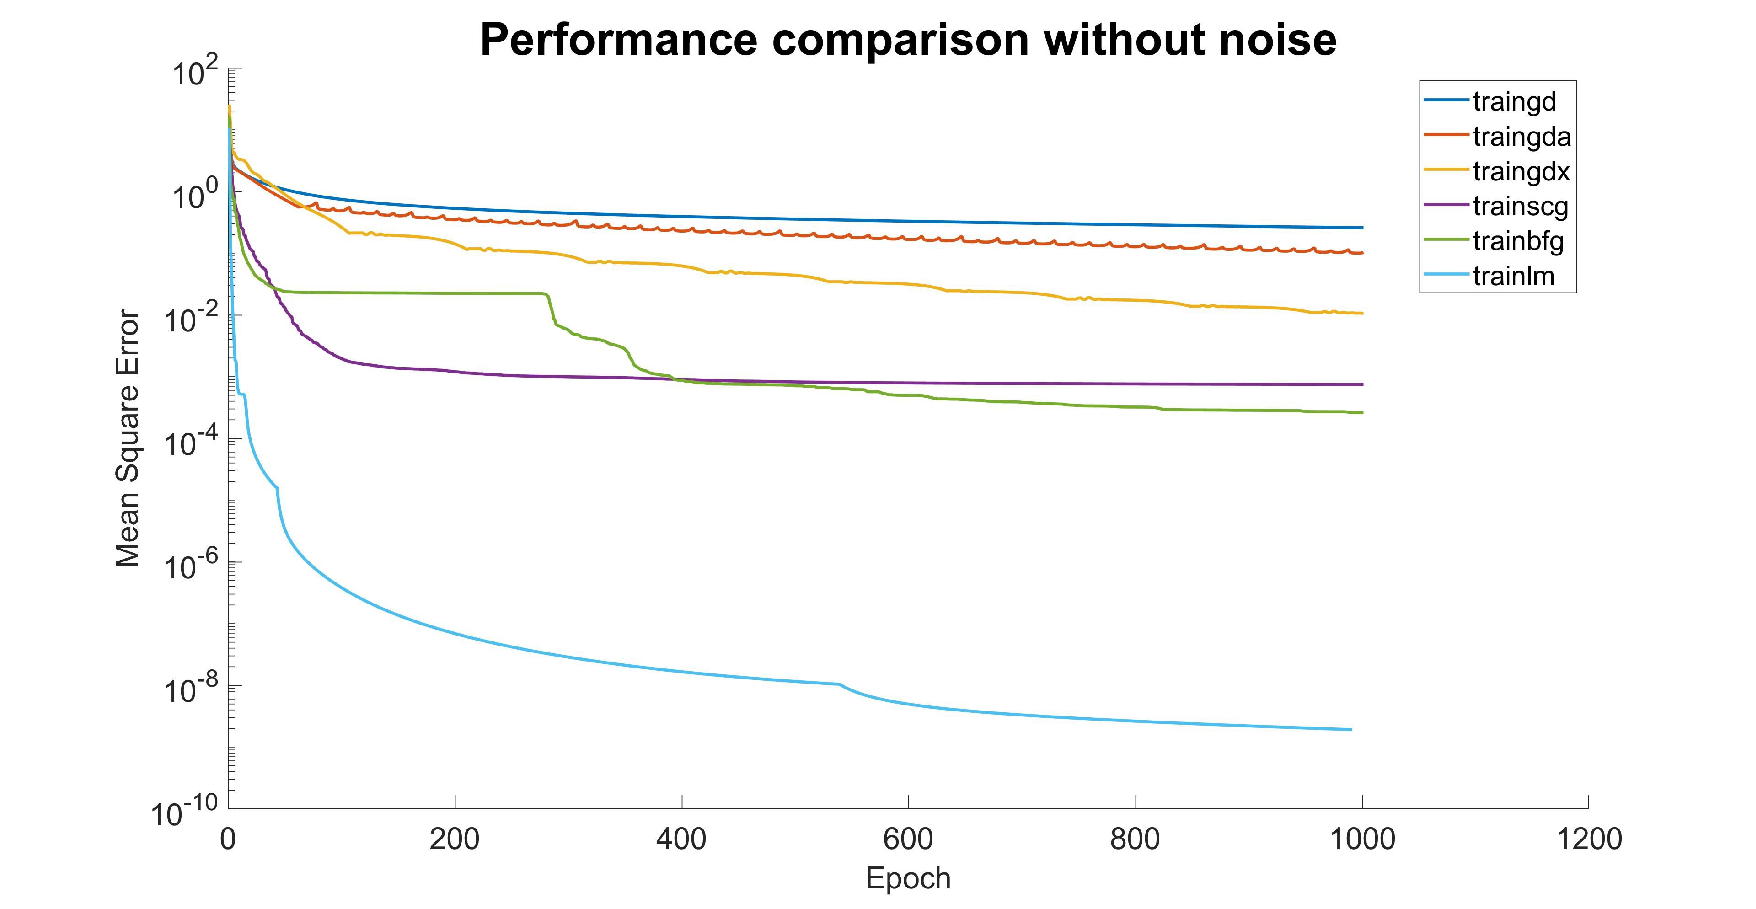
\includegraphics[width=\linewidth]{lab1/performancenonoise.pdf}
%  \caption{Various algorithm performance comparison on Sine function}
%  \label{fig:compare1}
%\end{subfigure}
%\caption{Sine function approx. without noise}
%\label{fig:fig}
%\end{figure}

\subsubsection{Function approximation comparison with noises}

In this section, we focus on how these algorithms perform on noisy data. In this case, we used \verb|randn| to add noise to our sine function. The standard deviation $\sigma$ of Gaussian noise is being adjusted in the experiments to change the noise level. Here we also need to be cautious of the over-fitting problem. The ideal neural network shall have the ability to approximate the underlying sine function curve instead of focusing too much on the noises. Also noted, in order to reduce the bias of the training dataset which has noises, here we increased the training sample size comparing to the clean data in prior.

Figure \ref{fig:noiselmgd} gives linear regression analysis on \verb|trainlm| and \verb|traingd|'s performances on noisy sine function approximation task. We noticed a slightly decreased correctness on \verb|traingd| but not on \verb|trainlm|. The next Figure \ref{fig:noiseperform} clearly illustrates the performance comparison on noisy data, \verb|trainlm| still works well but some other algorithms such as \verb|trainbfg| and \verb|trainscg| also achieved noticeable results by having very low MSEs.


\begin{figure}[h!]
  \centering
  % include third image
  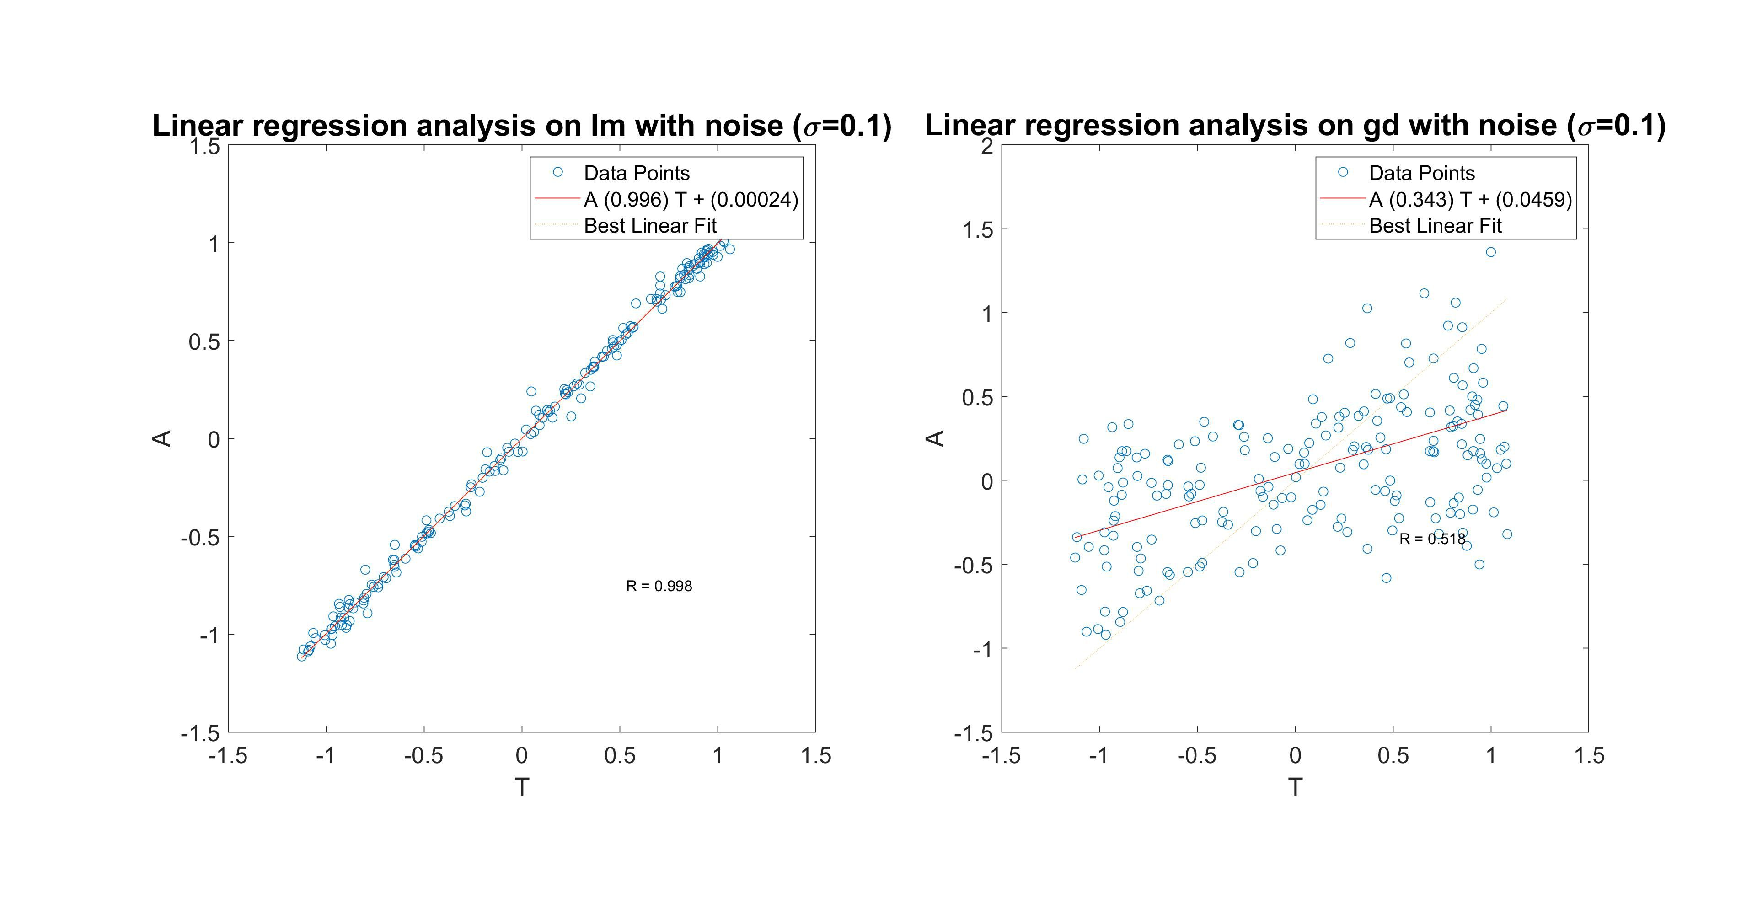
\includegraphics[width=\textwidth]{lab1/lmgdcomparewithnoise.pdf}
  \caption{Linear regression analysis on GD and LM (with noise)}
  \label{fig:noiselmgd}
\end{figure}

\begin{figure}[h!]
  \centering
  % include fourth image
  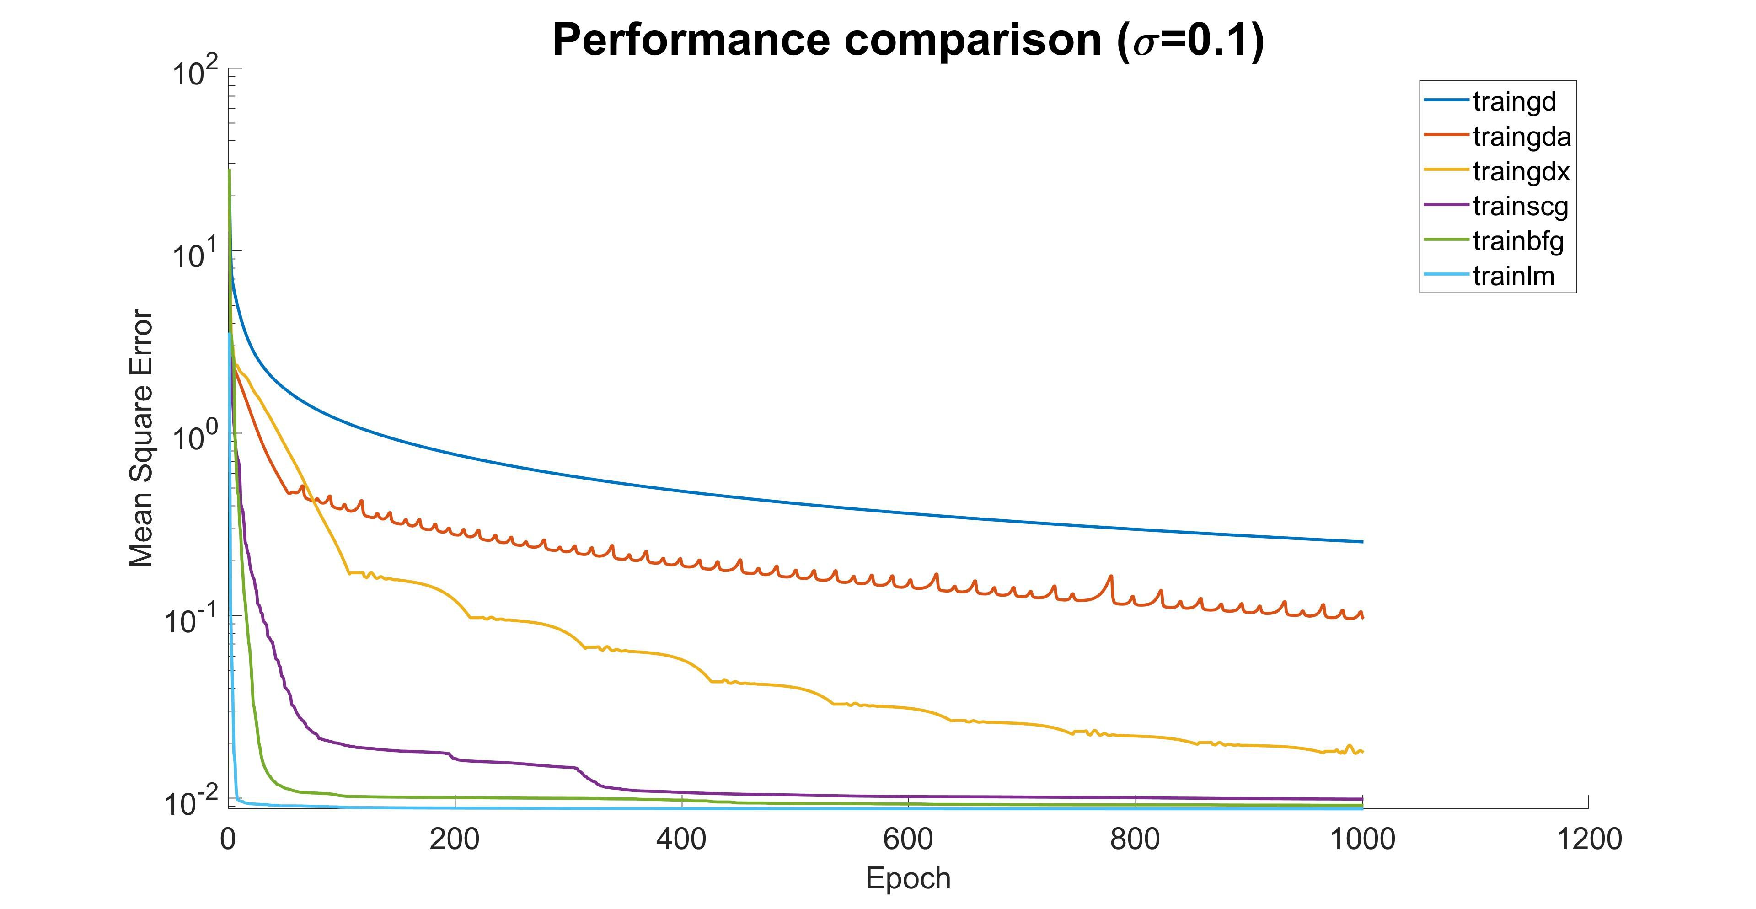
\includegraphics[width=\textwidth]{lab1/performancewithnoise.pdf}
  \caption{Performance comparison on Sine function (with noise)}
  \label{fig:noiseperform}
\end{figure}


%\begin{figure}[h!]
%\begin{subfigure}[b]{.49\textwidth}
%  \centering
  % include third image
%  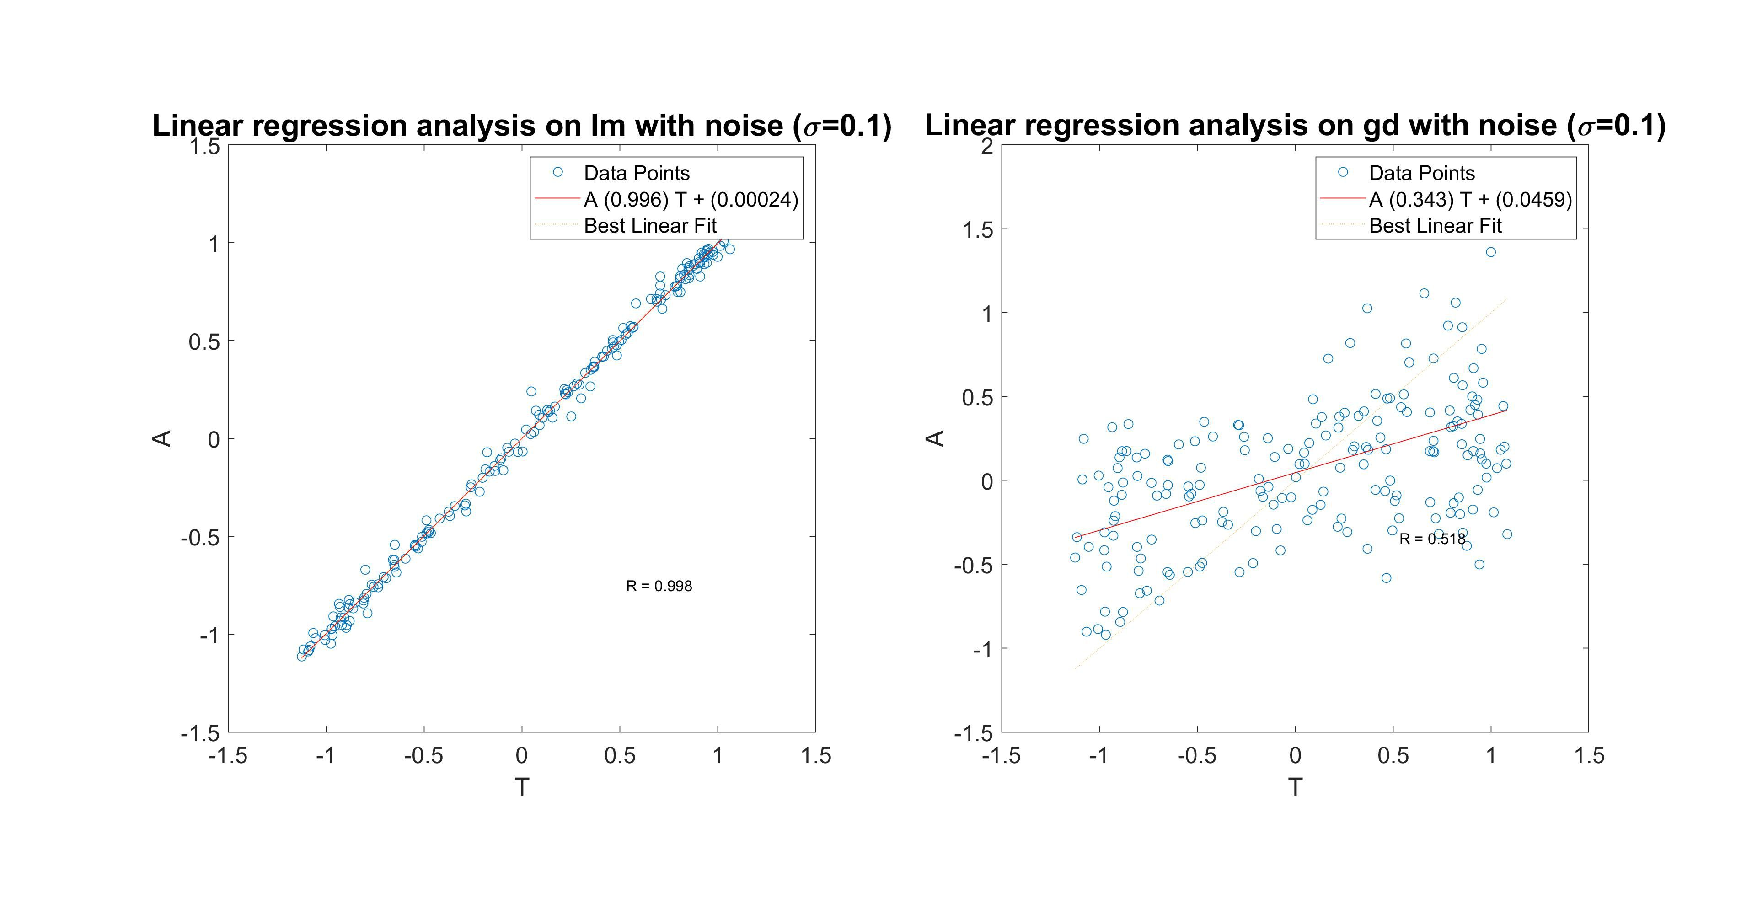
\includegraphics[width=\linewidth]{lab1/lmgdcomparewithnoise.pdf}
%  \caption{Linear regression analysis on GD and LM (with noise)}
%  \label{fig:noiselmgd}
%\end{subfigure}
%\hfill
%\begin{subfigure}[b]{.49\textwidth}
%  \centering
  % include fourth image
%  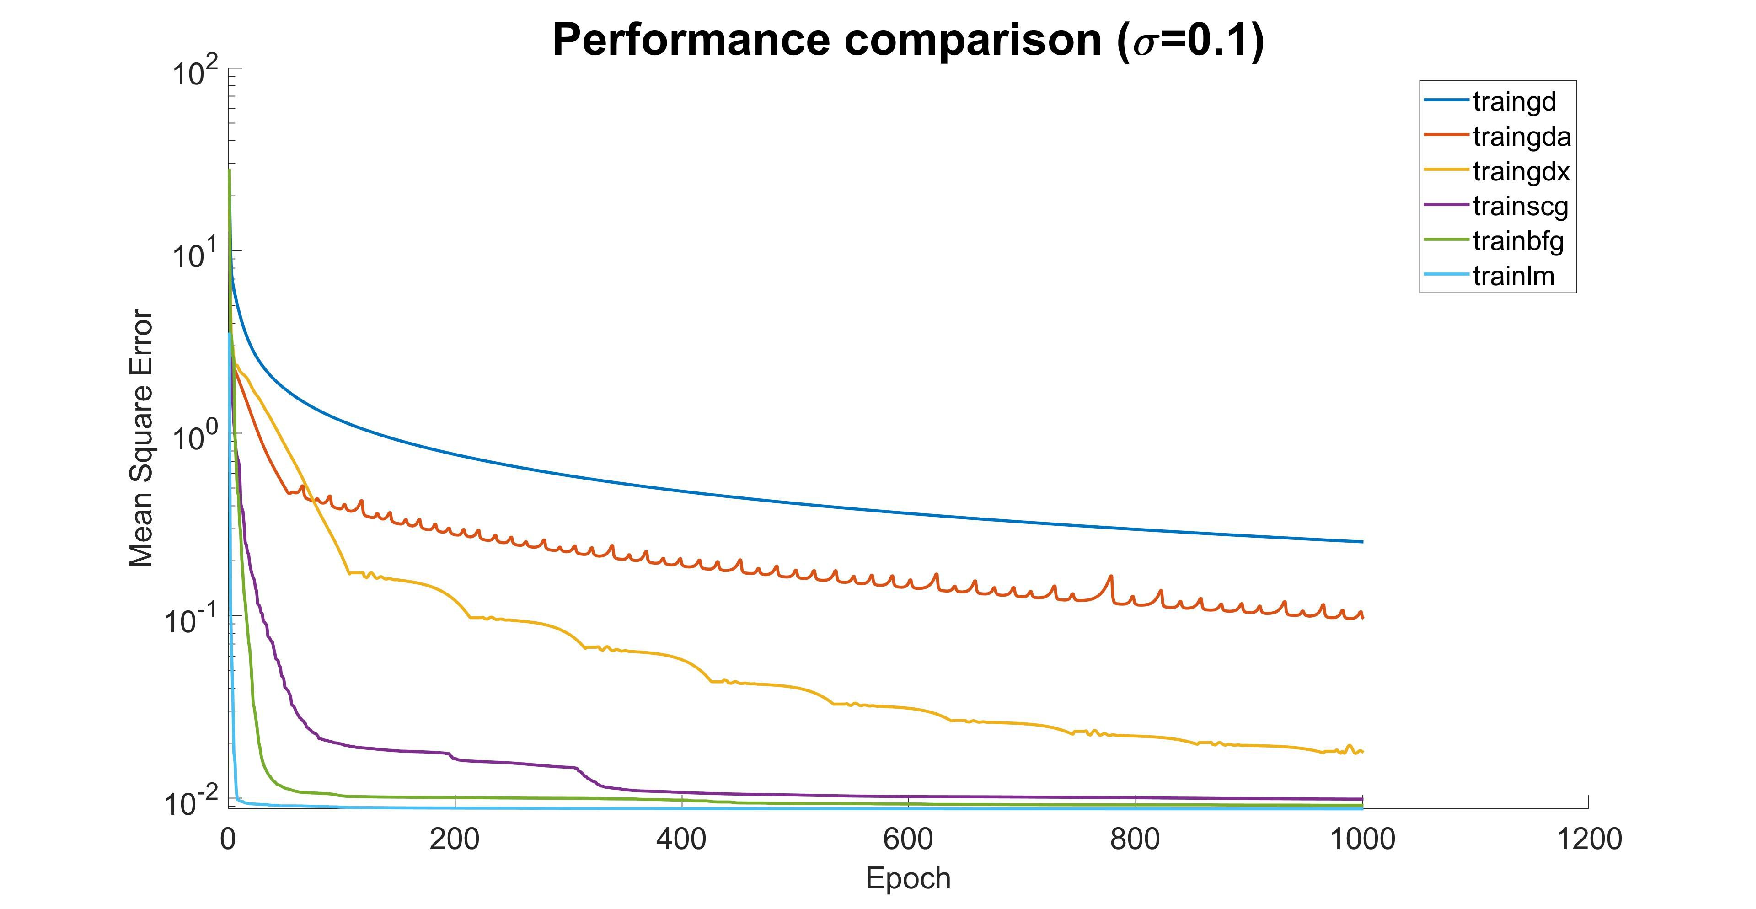
\includegraphics[width=\linewidth]{lab1/performancewithnoise.pdf}
%  \caption{Performance comparison on Sine function (with noise)}
%  \label{fig:noiseperform}
%\end{subfigure}
%\caption{Sine function approx. with noise}
%\label{fig:fig}
%\end{figure}

Now the question is how the noise level can affect the effectiveness of the training algorithms (neural network)? Here we show result on four different noise levels: $\sigma=0.1, 0.3, 0.4$ and $\sigma=0.5$. Figure \ref{fig:noise1} and Figure \ref{fig:noise5} illustrate how \verb|trainlm| and \verb|traingd| work on data with different noise levels. Surprisingly, it looks like \verb|trainlm| did get affected with high noise levels such as $\sigma=0.5$ and $\sigma=0.4$ but works just fine under low noise level as in $\sigma=0.1$ while \verb|traingd| has been seriously affected by all levels of noises.

Generally, increasing noise levels may decrease the R-value, and a well-tuned neural network shall have the ability to identify the actual underlying distribution of sine function and ignore those added irrelevant noises.

\begin{figure}[h!]
\begin{subfigure}[b]{.49\textwidth}
  \centering
  % include first image
  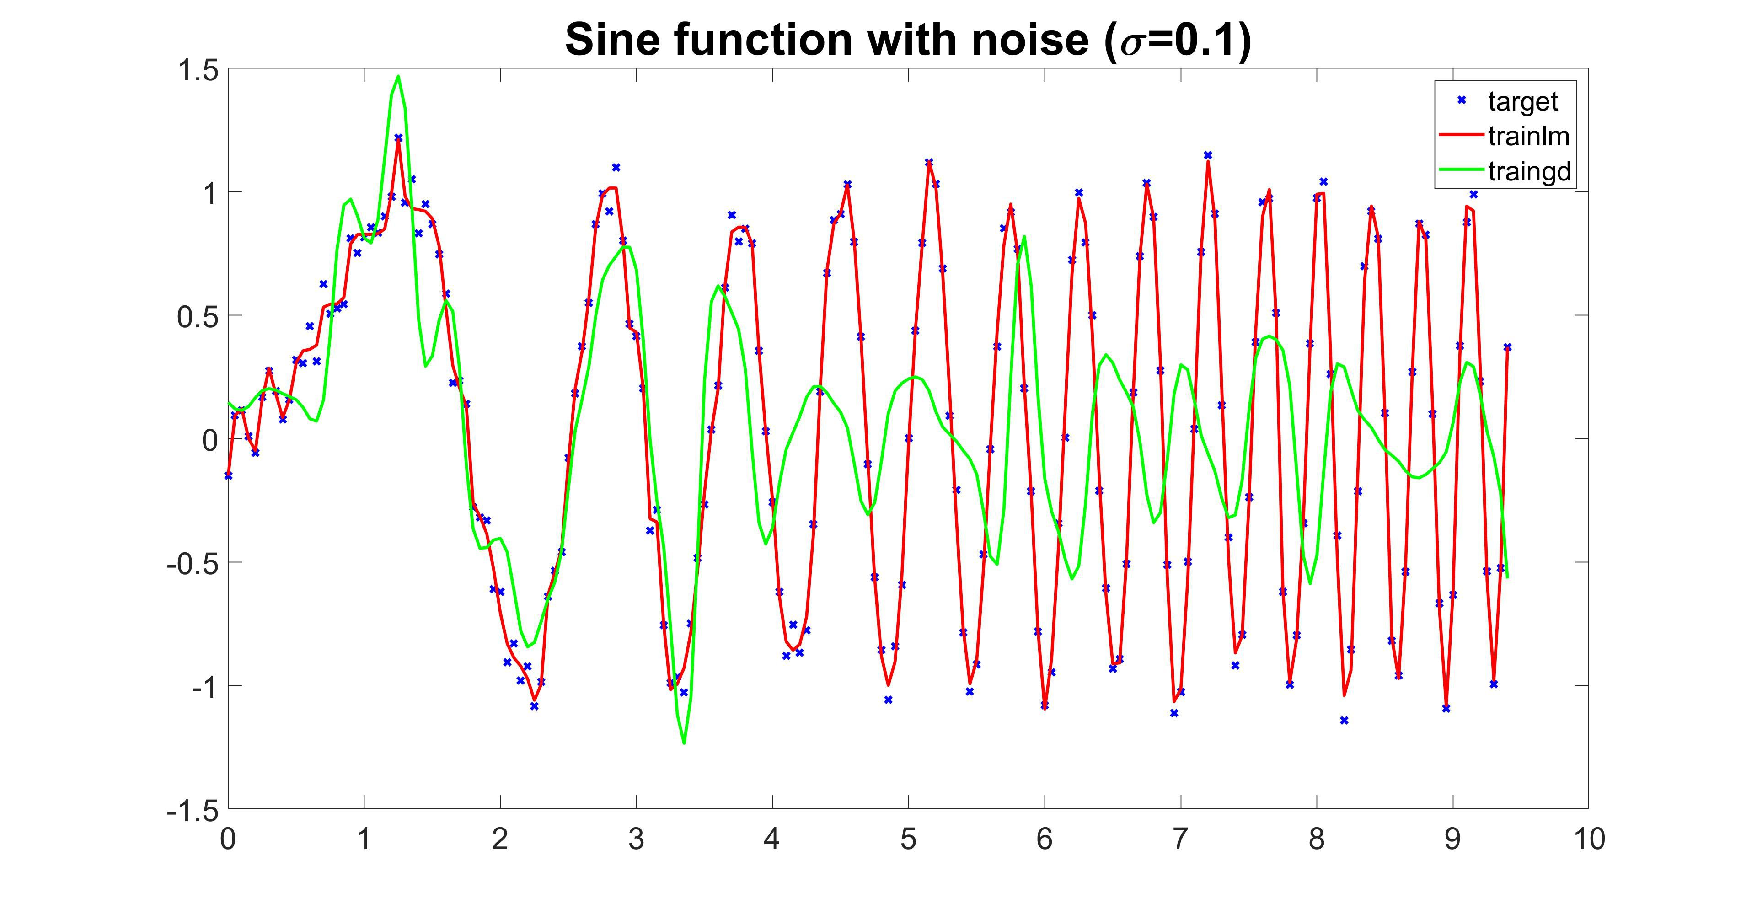
\includegraphics[width=\linewidth]{lab1/error1.pdf}
  \caption{Sine function approximation with noise (sigma=0.1)}
  \label{fig:noise1}
\end{subfigure}
\hfill
\begin{subfigure}[b]{.49\textwidth}
  \centering
  % include first image
  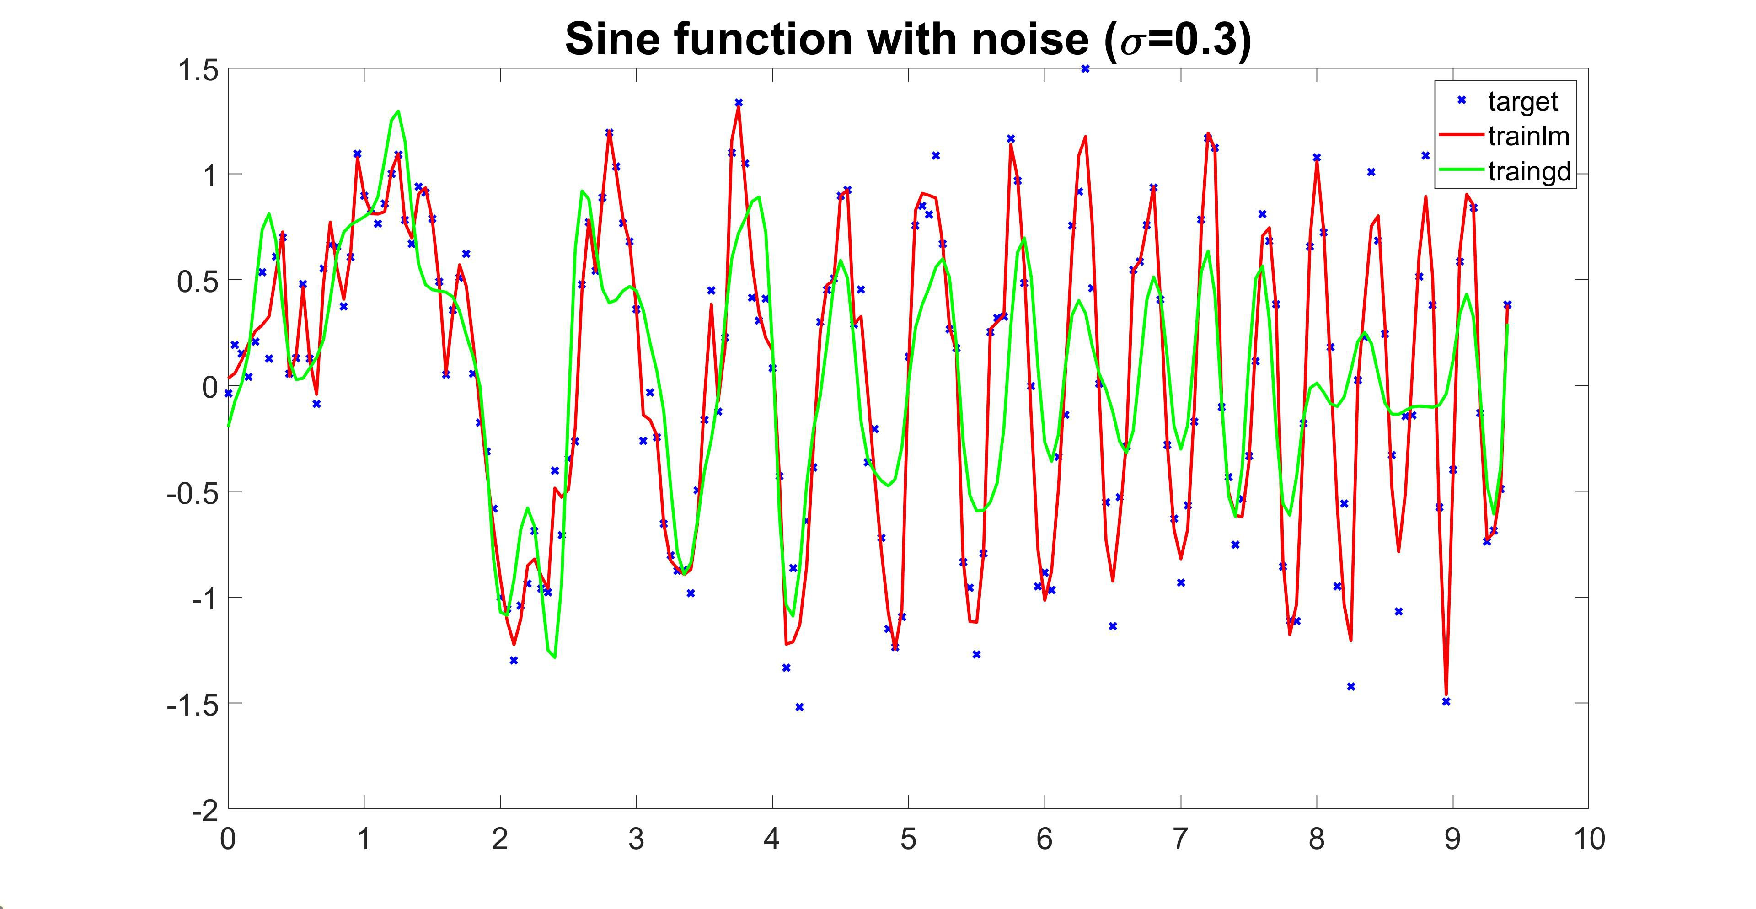
\includegraphics[width=\linewidth]{lab1/error3.pdf}
  \caption{Sine function approximation with noise (sigma=0.3)}
  \label{fig:noise3}
\end{subfigure}

\begin{subfigure}[b]{.49\textwidth}
  \centering
  % include first image
  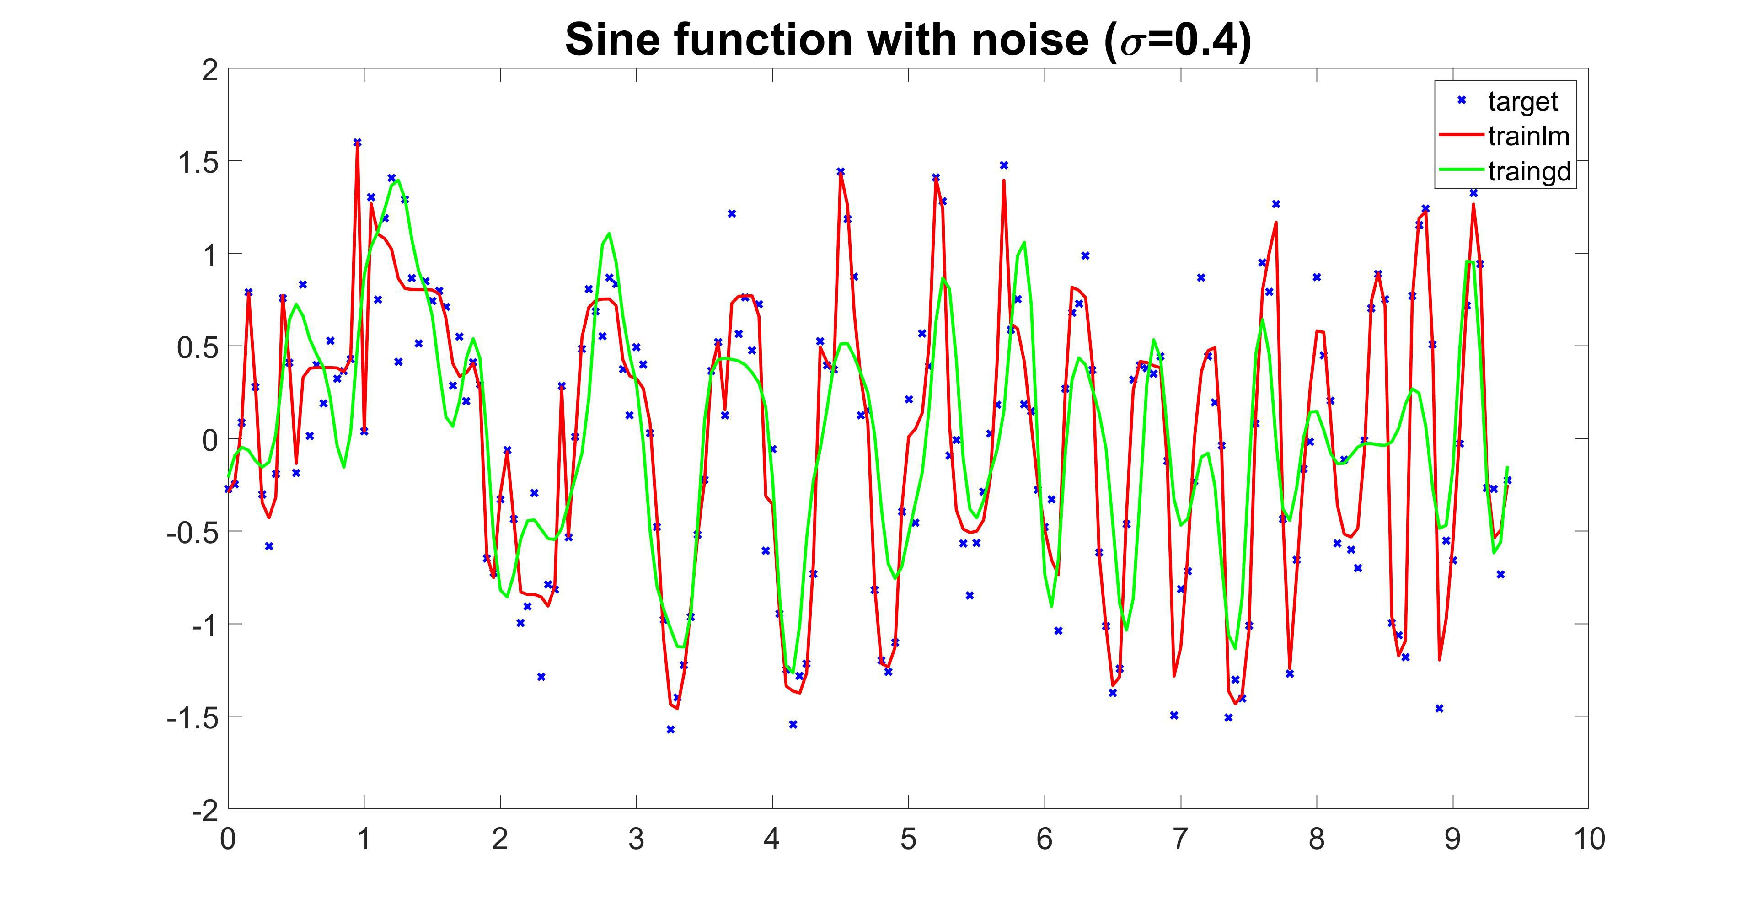
\includegraphics[width=\linewidth]{lab1/error4.pdf}
  \caption{Sine function approximation with noise (sigma=0.4)}
  \label{fig:noise4}
\end{subfigure}
\hfill
\begin{subfigure}[b]{.49\textwidth}
  \centering
  % include first image
  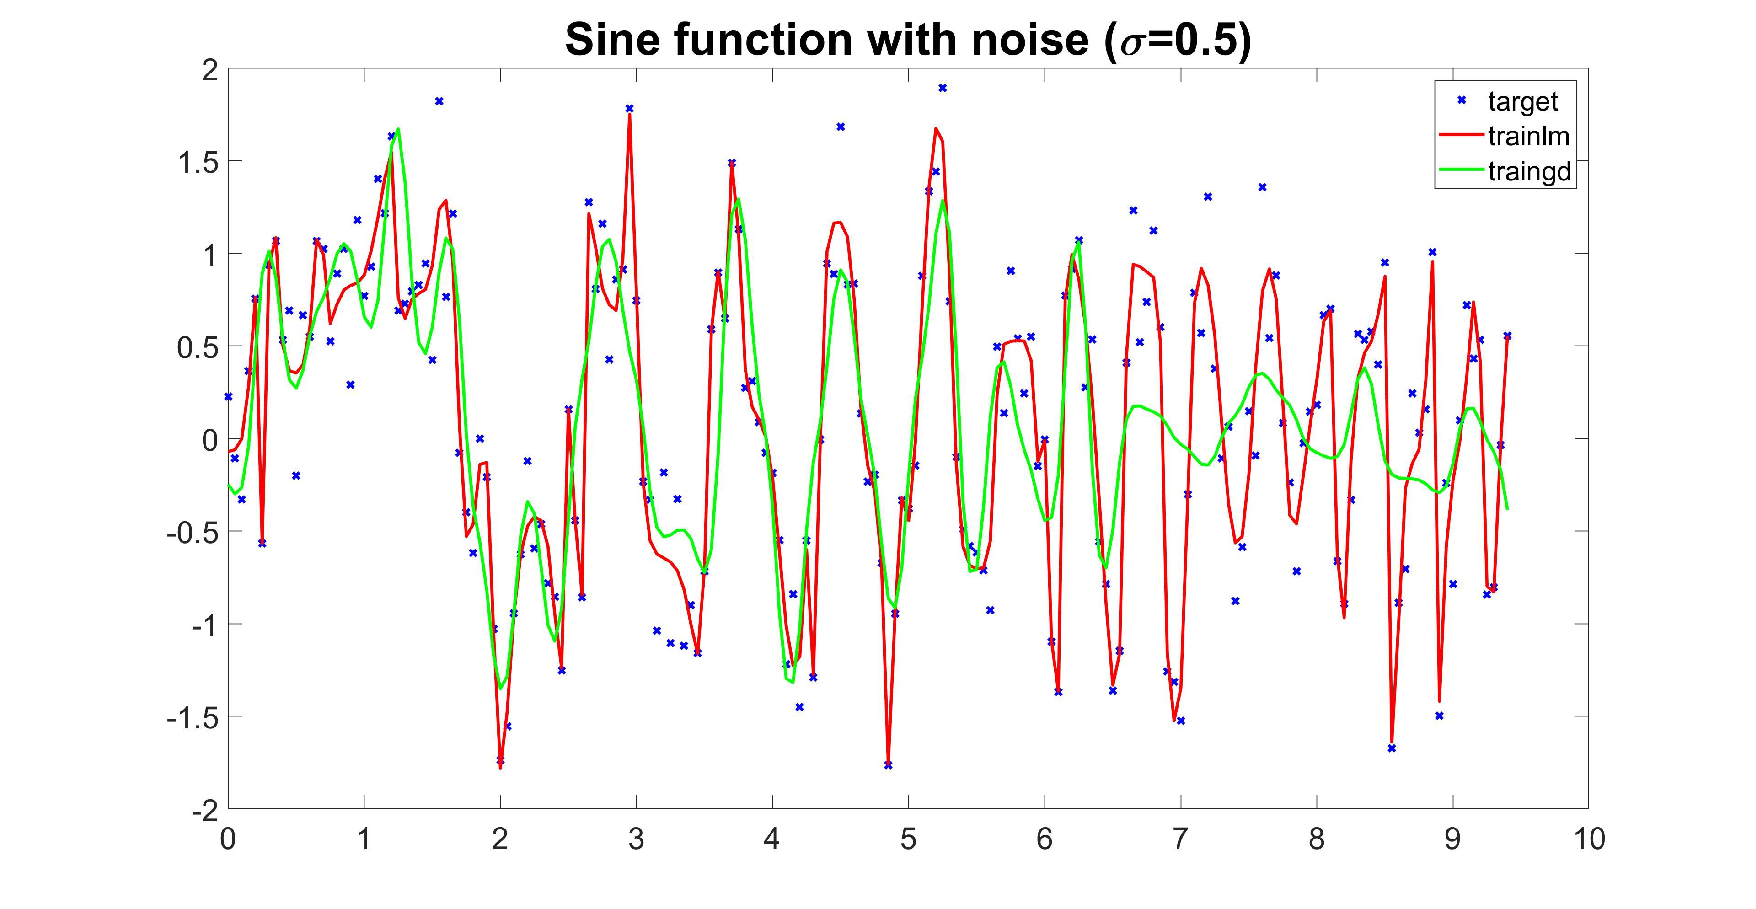
\includegraphics[width=\linewidth]{lab1/error5.pdf}
  \caption{Sine function approximation with noise (sigma=0.5)}
  \label{fig:noise5}
\end{subfigure}
\caption{Sine function approximation with noise}
\label{fig:noiseapprox}
\end{figure}


\subsection{Personal Regression}
Here, as my student number is r0728168, so I build my targets as follows:

$$
T_{new}=(8 T_1+7 T_2+6 T_3+2 T_4+1 T_5) /(8+7+6+2+1)
$$

My dataset consists of $X_1$, $X_2$ and $T_{new}$. As told in the assignment requirement: ``draw 3 (independent) samples of 1,000
points each, use them as the training set, validation set, and test set, respectively. ''

As we all know that the accuracy at the end of our training procedure does not always tell us much about whether our model is any good. We can make sufficiently complex models fit completely arbitrary training data without actually learning anything whatsoever. To evaluate whether our model is learning something interesting, we want to test it on the testing data. Figure \ref{fig:trainsurface} plots the surfaces of my training set and testing set.

\begin{figure}[h!]
\begin{subfigure}[b]{.49\textwidth}
  \centering
  % include first image
  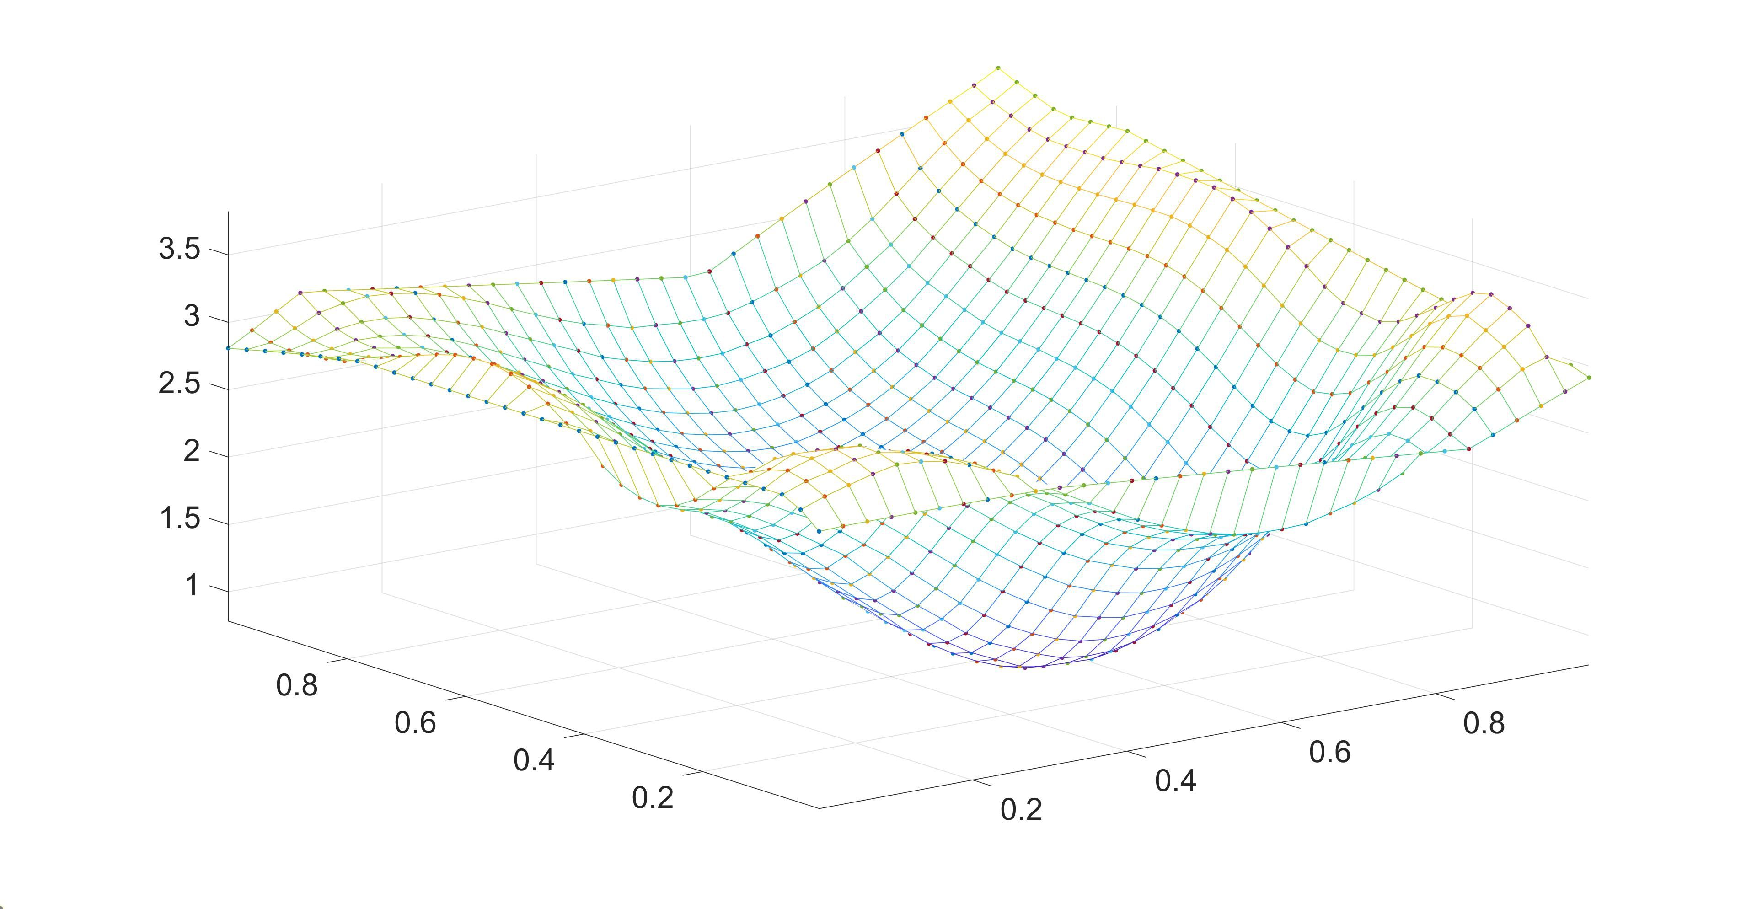
\includegraphics[width=\linewidth]{lab1/personaltrainsurface.pdf}
  \caption{Surface of training set}
  \label{fig:trainsurface}
\end{subfigure}
\hfill
\begin{subfigure}[b]{.49\textwidth}
  \centering
  % include first image
  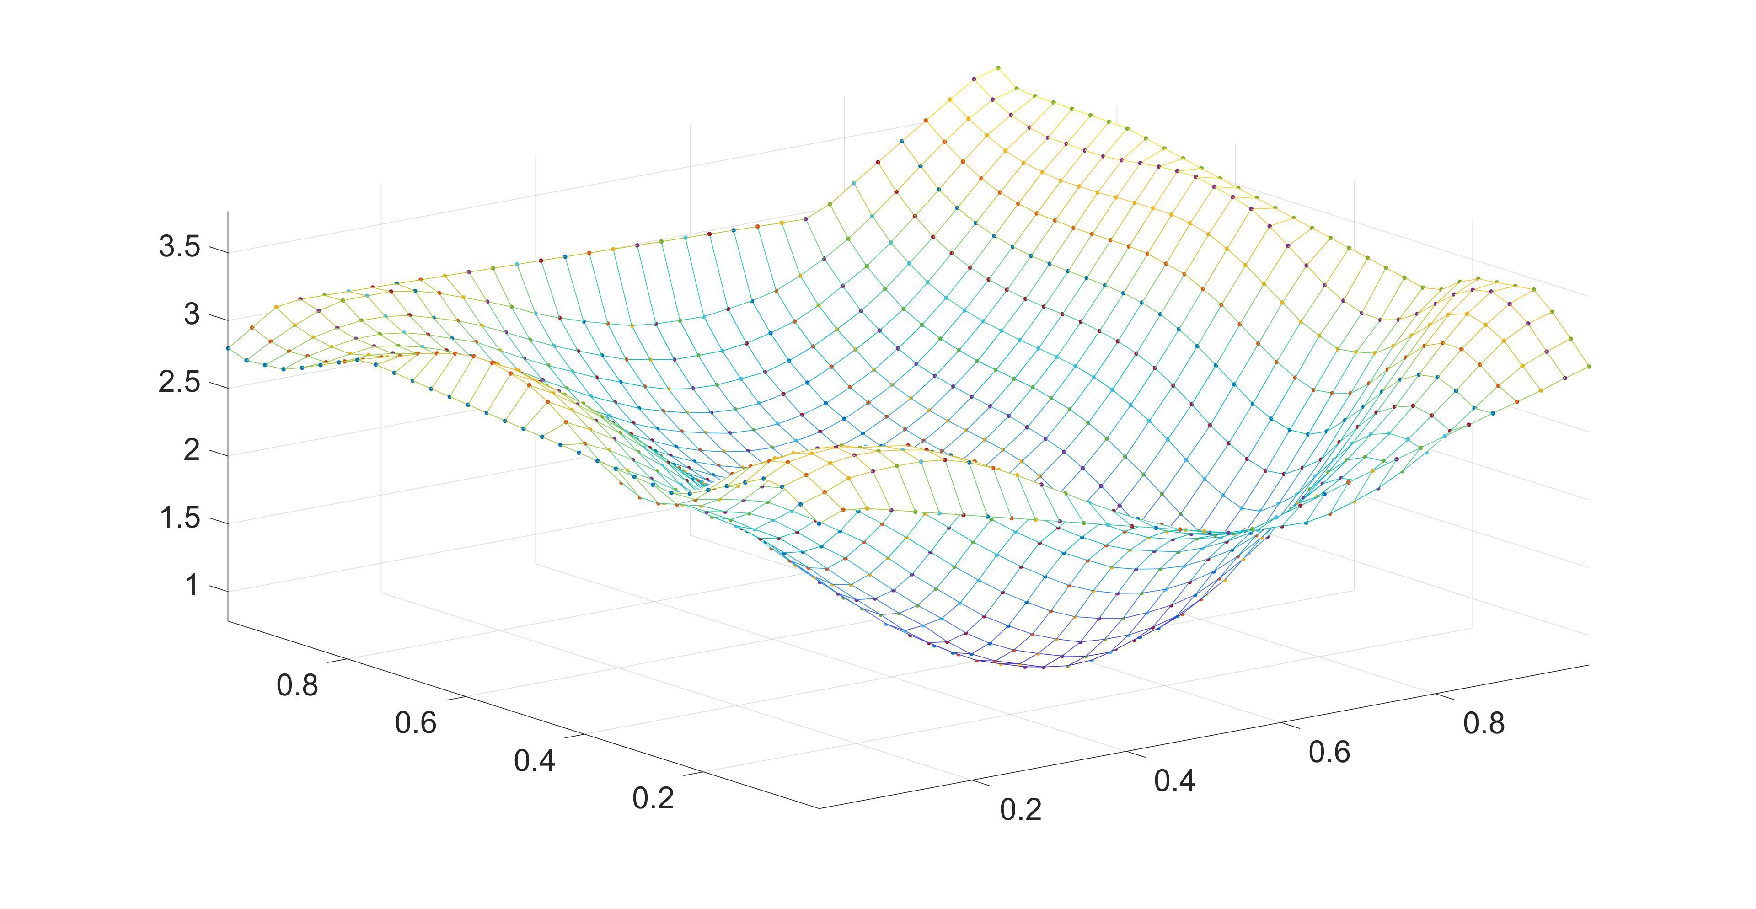
\includegraphics[width=\linewidth]{lab1/personaltestsurface.pdf}
  \caption{Surface of testing set}
  \label{fig:testsurface}
\end{subfigure}
\caption{Surfaces of datasets}
\label{fig:fig}
\end{figure}

In general, choosing the size, number and form of hidden layers, is a difficult problem which depends on the type and amount of data we have, as well as the computational resources available to us. A lot of trial and error usually goes into finding a good architecture.

Here, aiming to use a simple structure and avoid over-fitting as much as possible, we adopted a single hidden layer and tested on different numbers of hidden neurons. Figure \ref{fig:hidden} presents the curve of hidden neurons versus Mean Squared Error. More hidden neurons usually means more computational costs: time and memory use, and very deep neural networks also have more risks on over-fitting. Here we chose the number of 51 hidden neurons as it has the smallest MSE regionally. More hidden neurons may look like the MSE has been reduced, but it can be caused by over-fitting.

\begin{figure}[h!]
  \centering
  % include second image
  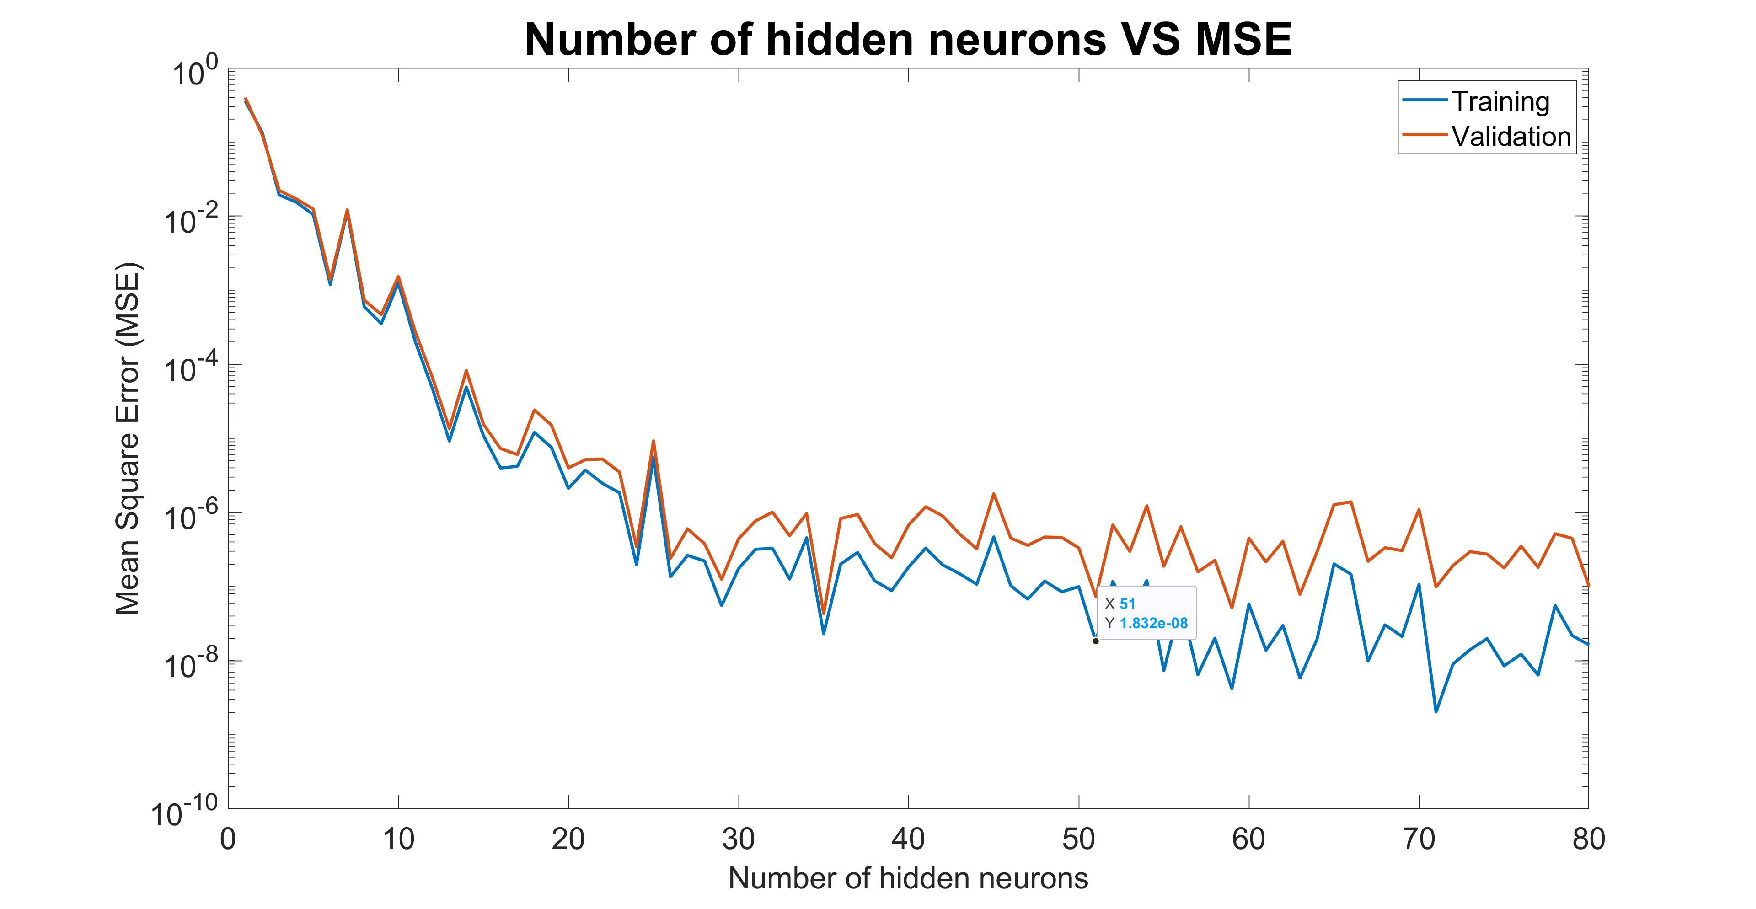
\includegraphics[width=\textwidth]{lab1/hiddenneuron.pdf}
  \caption{Number of hidden units Versus MSE}
  \label{fig:hidden}
\end{figure}

Below Figure \ref{fig:error} demonstrates the error surface between the prediction and our testing data points - ground truth. Our MSE for this testing set is 1.6925e-08=0.000000016925 which is very small, may indicate a good fit.

\begin{figure}[h!]
  \centering
  % include second image
  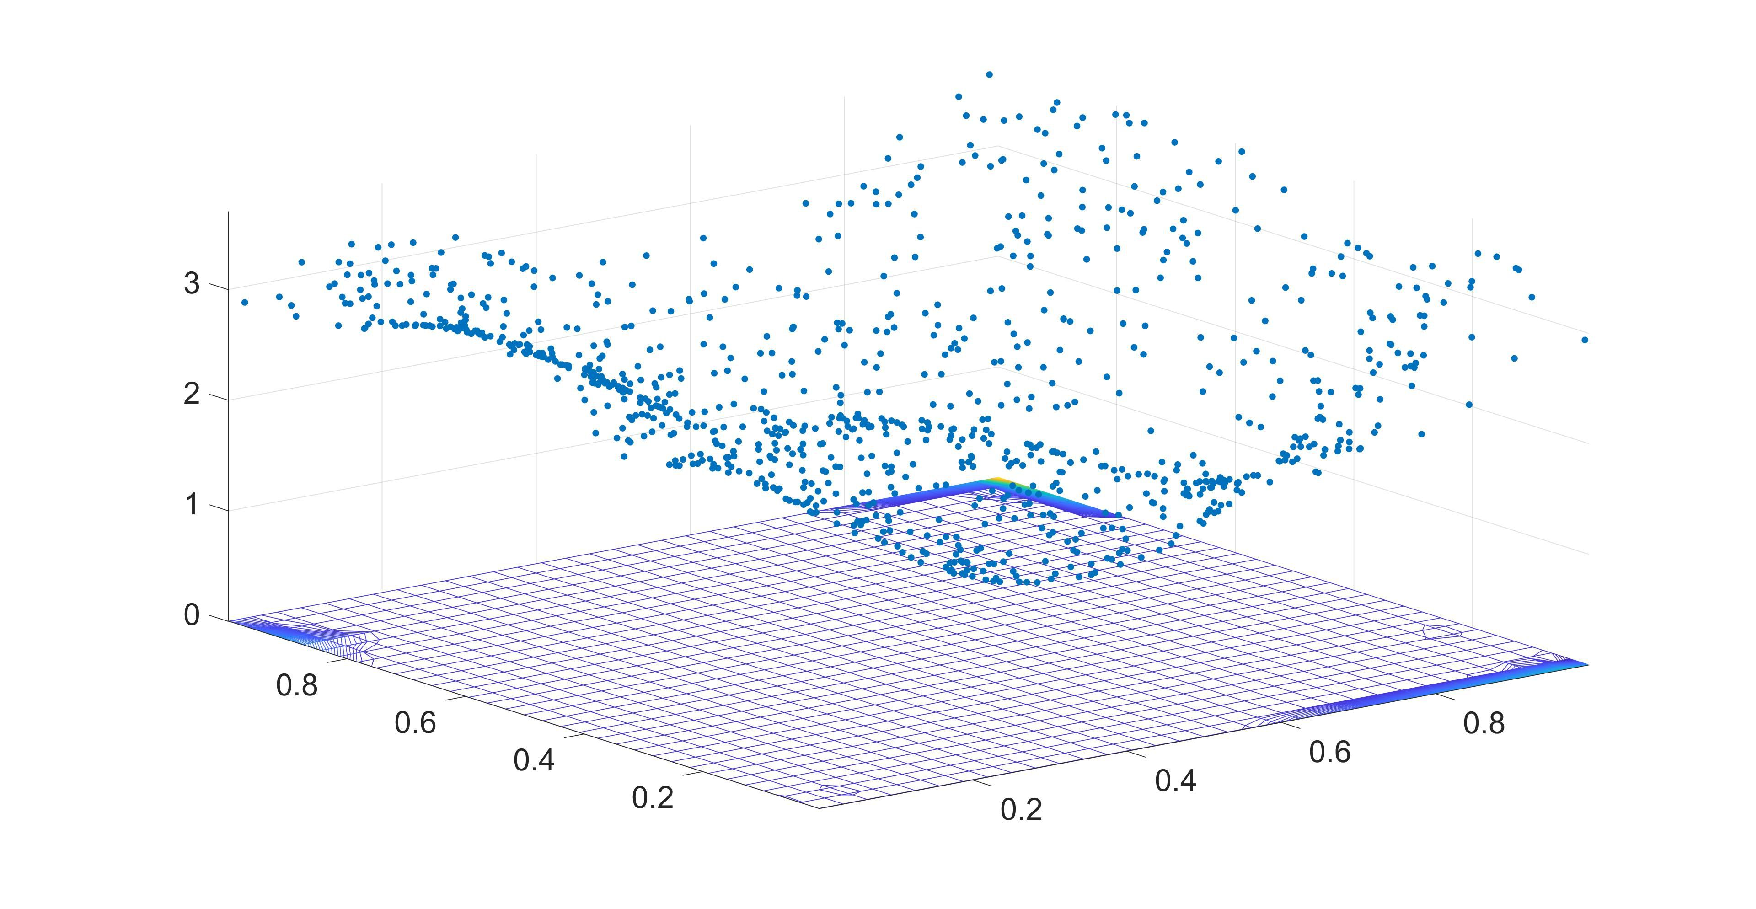
\includegraphics[width=\textwidth]{lab1/errorsurface.pdf}
  \caption{Error surface with testing data points}
  \label{fig:error}
\end{figure}

\subsection{Bayesian inference of network hyper-parameters}

In order to make the back-propagation process more robust and reduce the widely used process of cross-validation, we prefer to adopt Bayesian regularised neural networks. Bayesian regularisation can convert nonlinear regression functions into a clear and more regular form such as ridge regressions. This hugely benefits the training process which can get rid of the unnecessary validation part, for instance, back-propagation.

Figure \ref{fig:brlmnonoise} and Figure \ref{fig:brlmwithnoise} shows the linear regression analysis on both \verb|trainbr| and \verb|trainlm| running on noisy and non-noisy data. It is interesting to see that noise does not affect much.

\begin{figure}[h!]
  \centering
  % include second image
  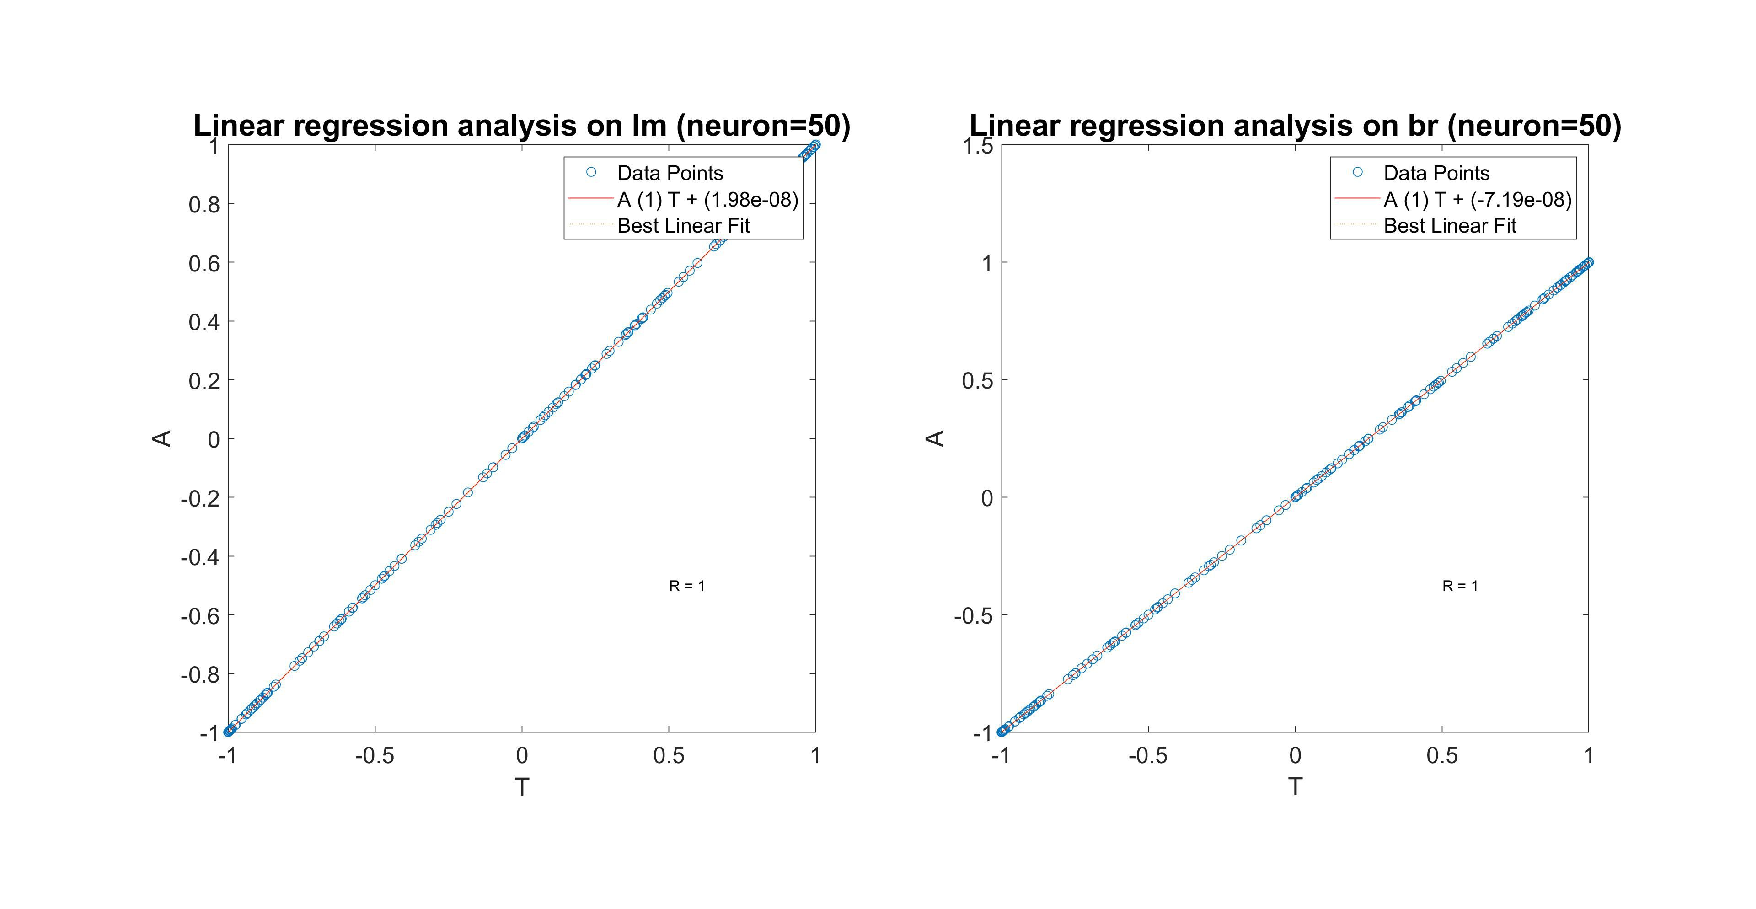
\includegraphics[width=\textwidth]{lab1/nonoisetrainbrcompare.pdf}
  \caption{Linear regression analysis on lm and br}
  \label{fig:brlmnonoise}
\end{figure}

\begin{figure}[h!]
  \centering
  % include second image
  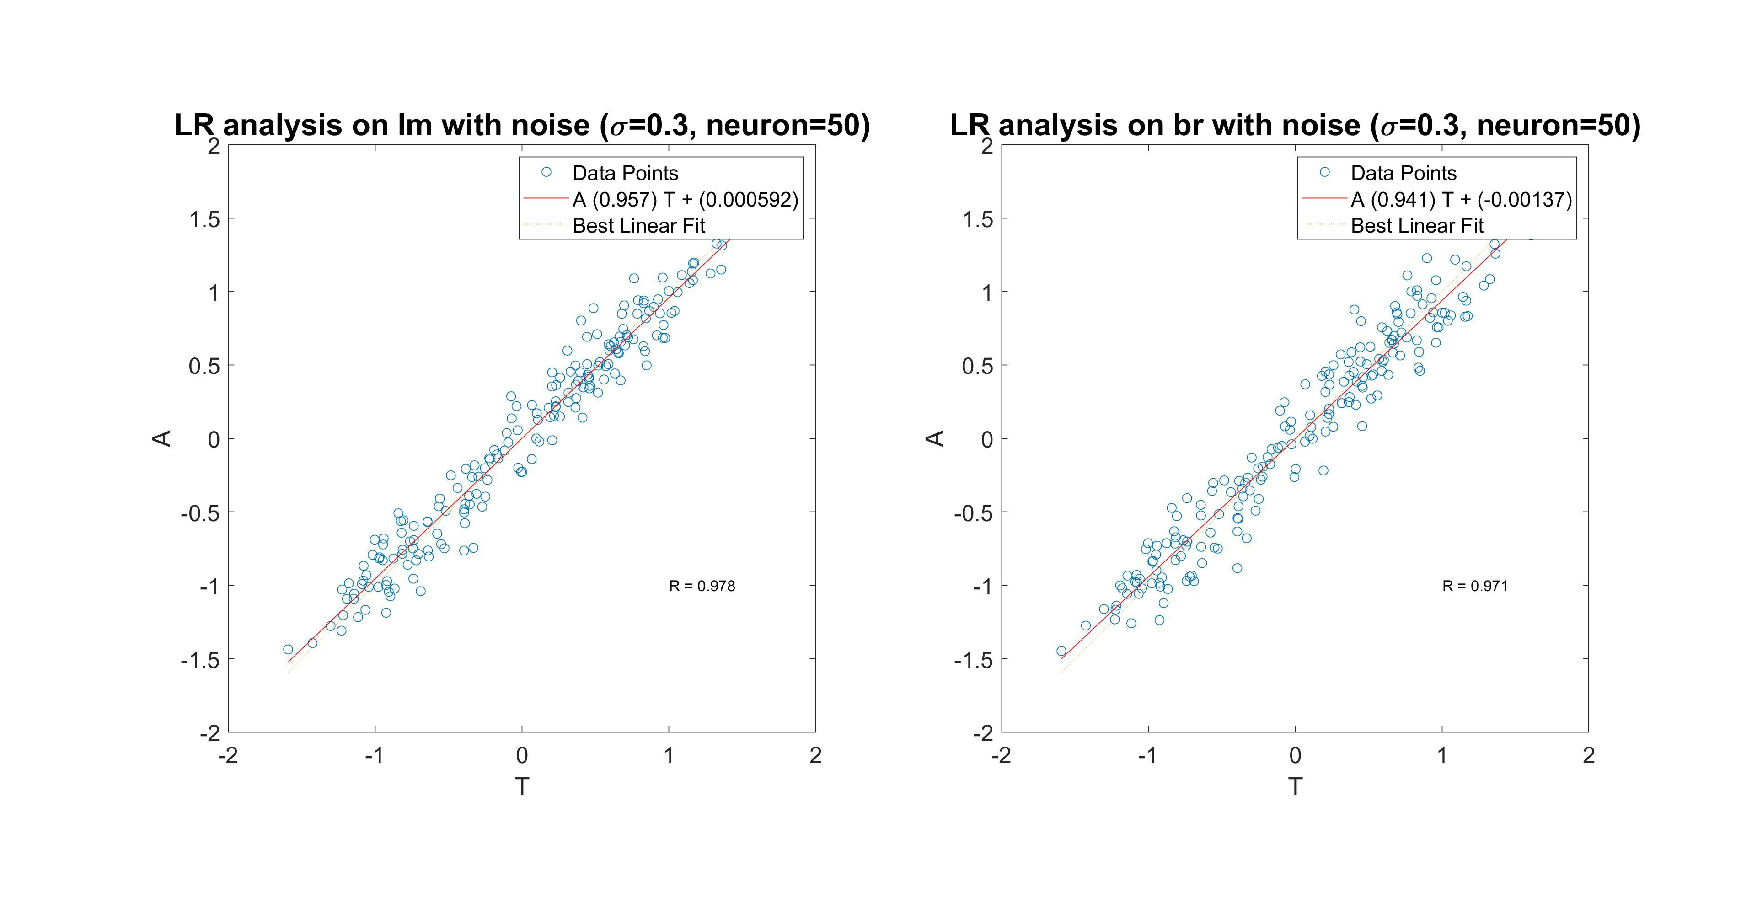
\includegraphics[width=\textwidth]{lab1/noisetrainbrcompare.pdf}
  \caption{Linear regression analysis on lm and br with noise}
  \label{fig:brlmwithnoise}
\end{figure}

Next, we perform experiments on different numbers of hidden neurons and check how \verb|trainbr| works under over-parametrised networks. Here we use 40 neurons (Figure \ref{fig:br40}) and 70 neurons (Figure \ref{fig:br70}) on noise-less data first, we noticed that for over-parametrised networks, the fit looks better but this may because of the increased flexibility - the risk of over-fitting in the meantime. However, \verb|trainbr| is able to avoid over-fitting, but the trade-off is over-consumed computational power: much more time used. \verb|trainlm| can achieve excellent results on most cases too but its trade-off is also its high computational memory need. For noisy data, it does not seem evident that \verb|trainbr| have a definite advantage among others.


\begin{figure}[h!]
\begin{subfigure}[b]{.49\textwidth}
  \centering
  % include first image
  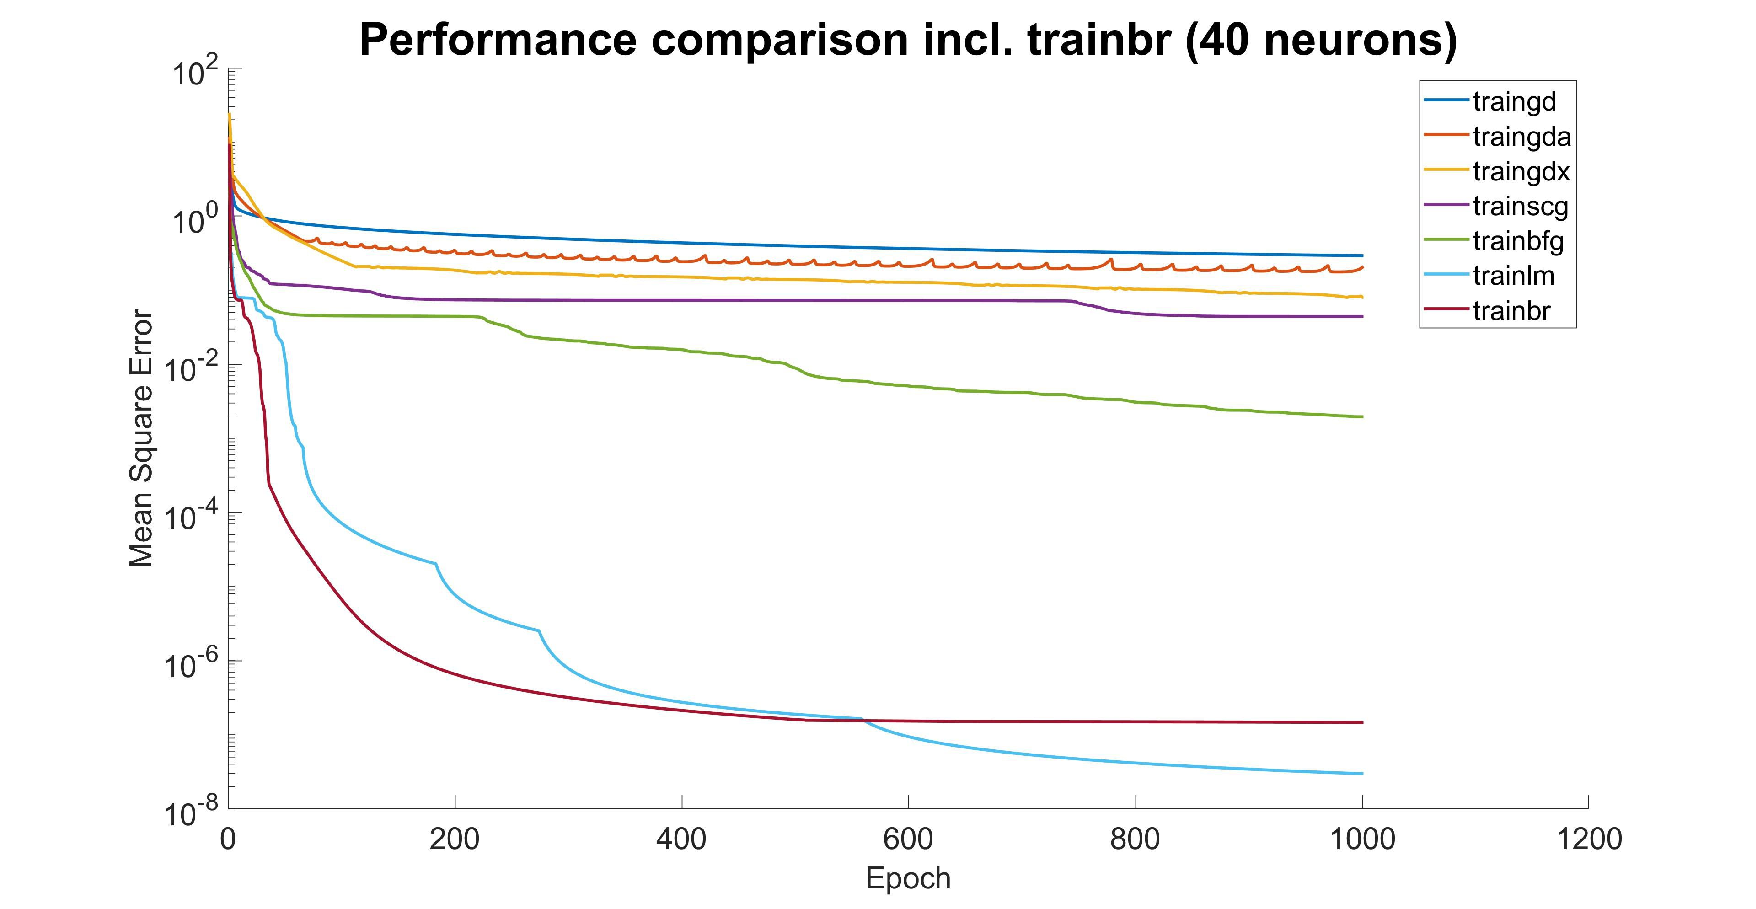
\includegraphics[width=\linewidth]{lab1/trainbr40.pdf}
  \caption{Performance comparison (neuron=40)}
  \label{fig:br40}
\end{subfigure}
\hfill
\begin{subfigure}[b]{.49\textwidth}
  \centering
  % include first image
  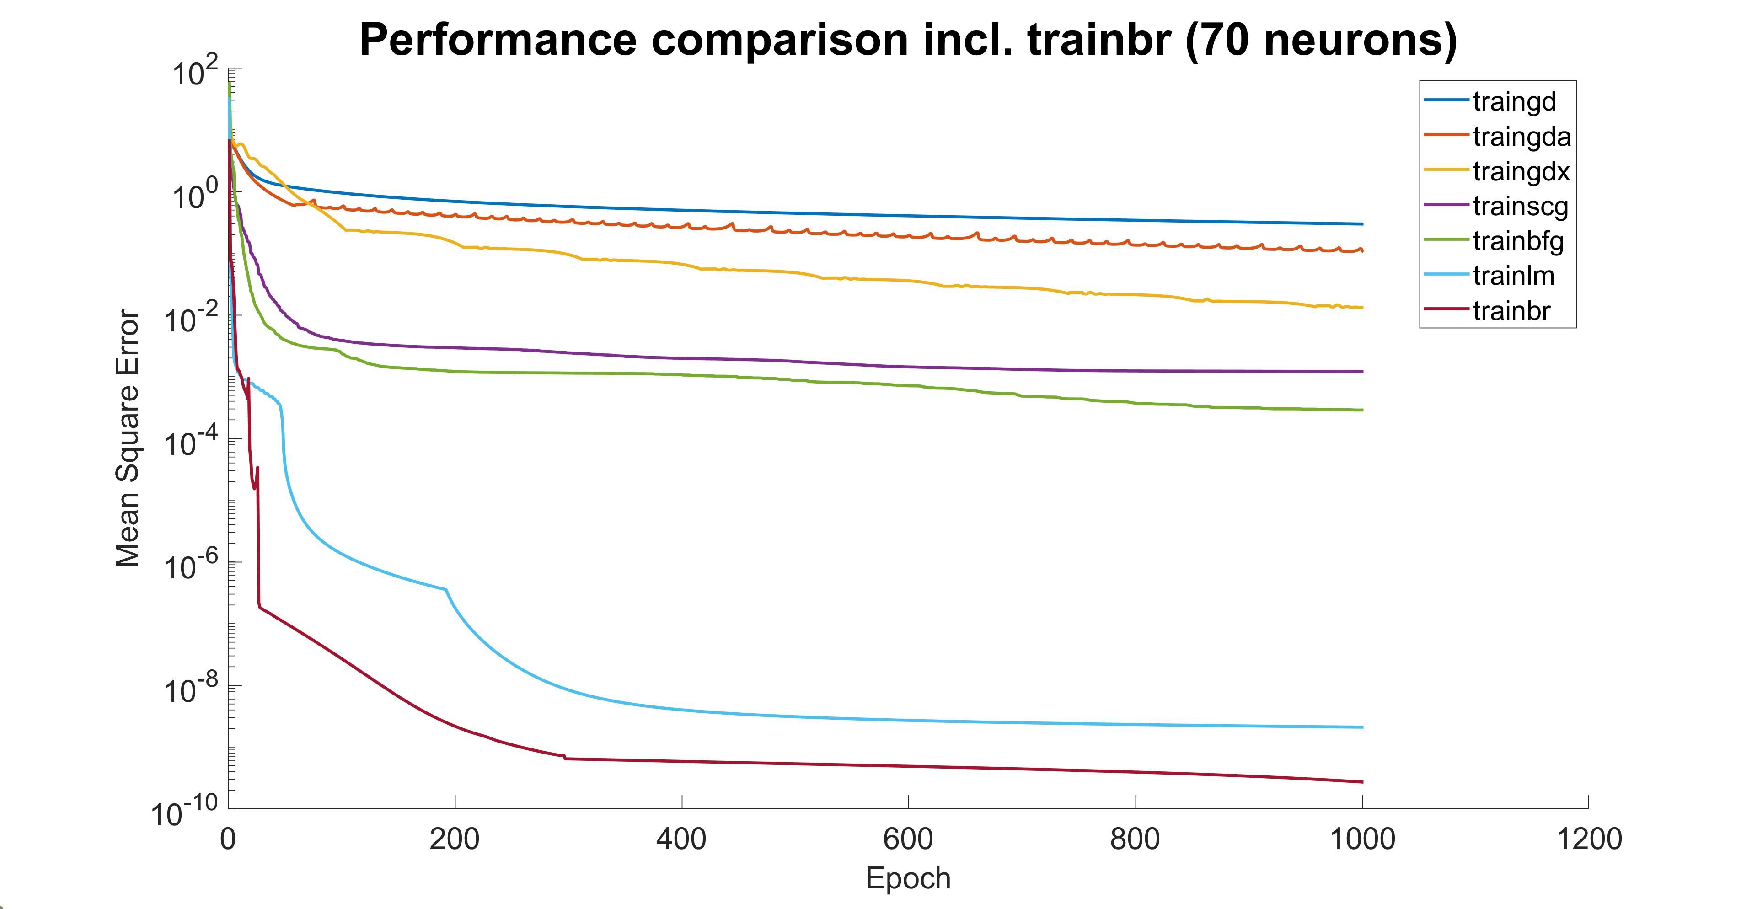
\includegraphics[width=\linewidth]{lab1/trainbr70.pdf}
  \caption{Performance comparison (neuron=70)}
  \label{fig:br70}
\end{subfigure}
\caption{Performance comparison without noise incl. trainbr}
\label{fig:fig}
\end{figure}

\begin{figure}[h!]
\begin{subfigure}[b]{.49\textwidth}
  \centering
  % include first image
  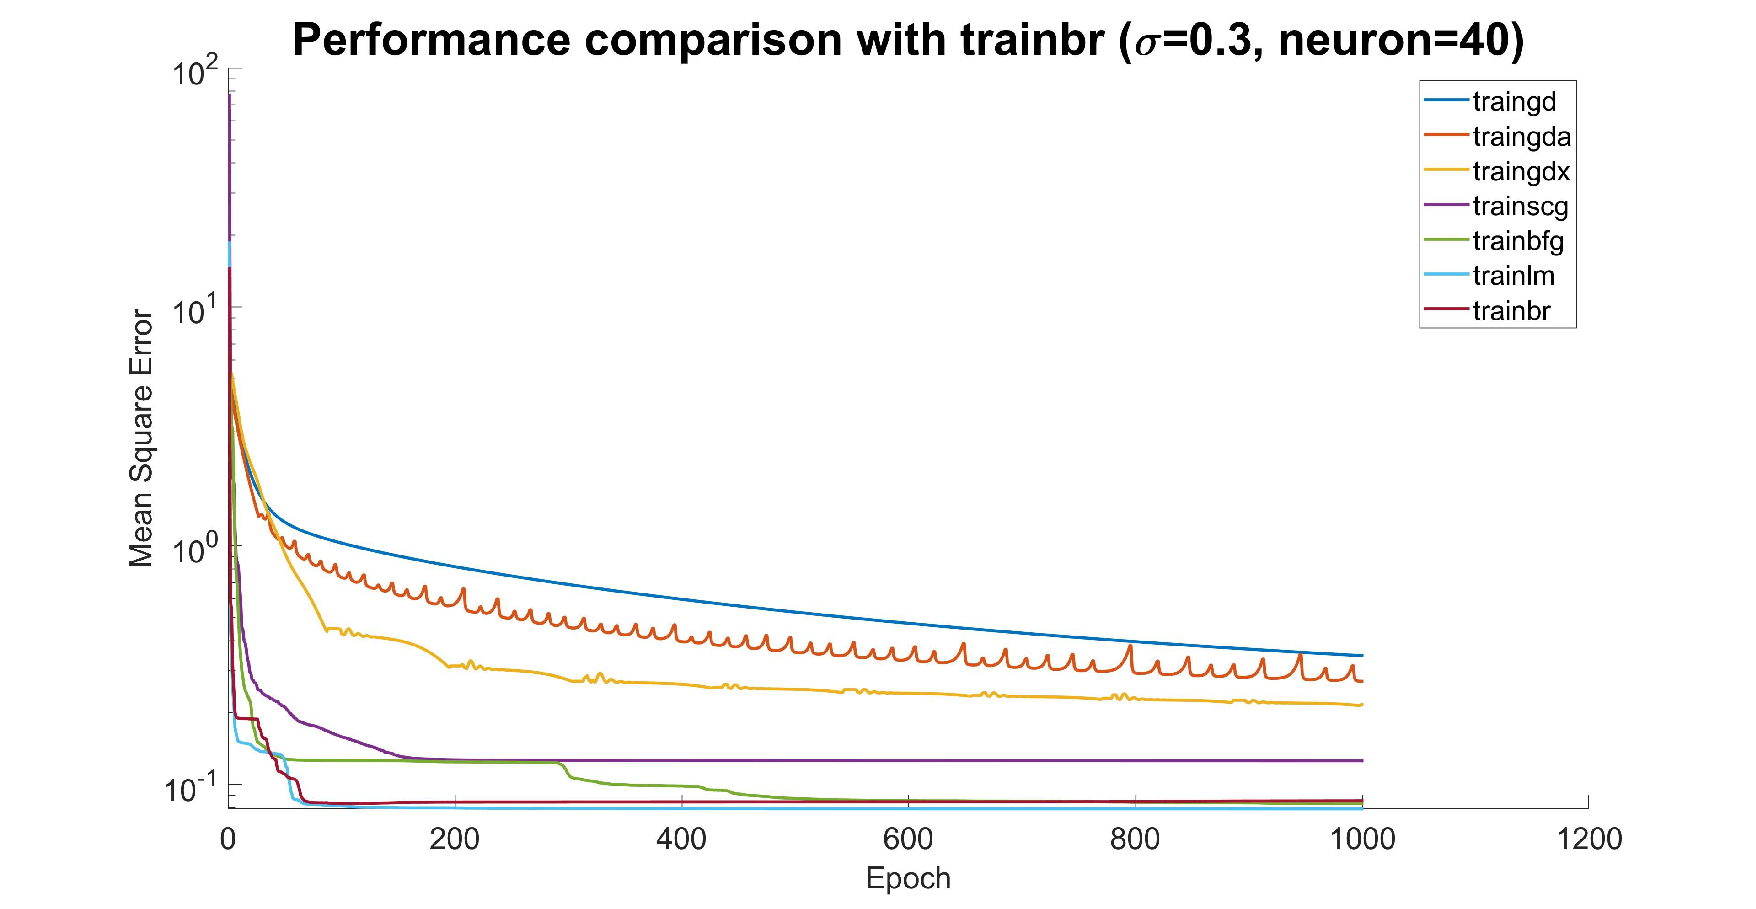
\includegraphics[width=\linewidth]{lab1/trainbr40noise.pdf}
  \caption{Performance comparison with noise (neuron=40)}
  \label{fig:noisebr40}
\end{subfigure}
\hfill
\begin{subfigure}[b]{.49\textwidth}
  \centering
  % include first image
  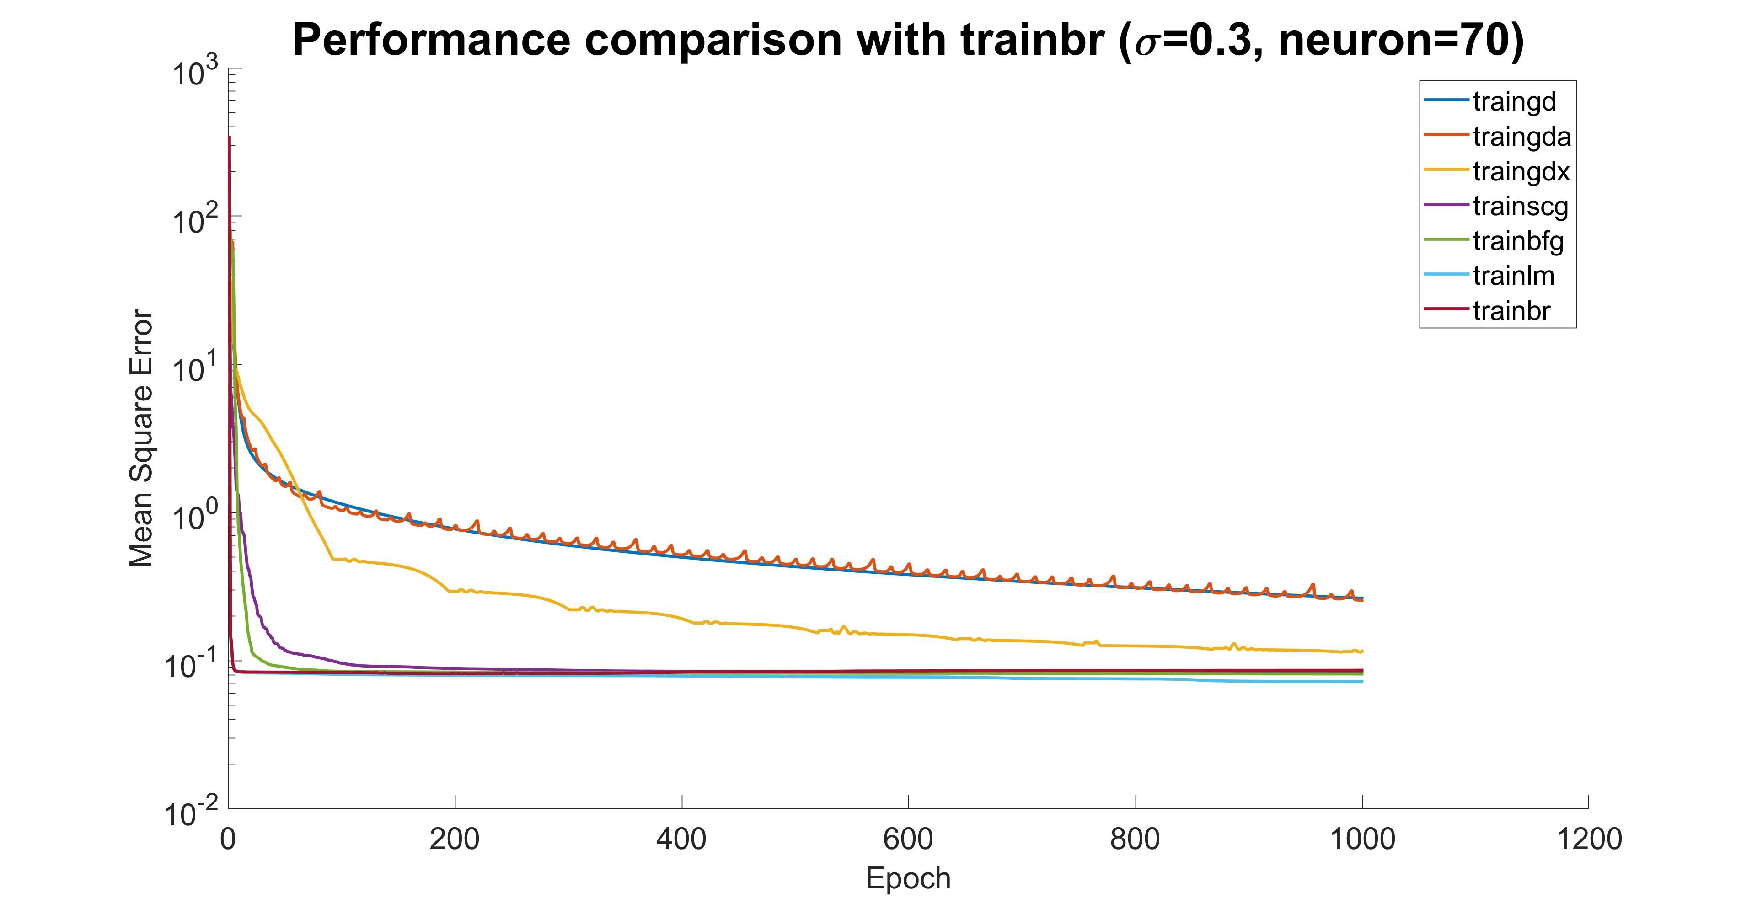
\includegraphics[width=\linewidth]{lab1/trainbr70noise.pdf}
  \caption{Performance comparison with noise (neuron=70)}
  \label{fig:noisebr70}
\end{subfigure}
\caption{Performance comparison with noise incl. trainbr}
\label{fig:fig}
\end{figure}

\begin{figure}[h!]
  \centering
  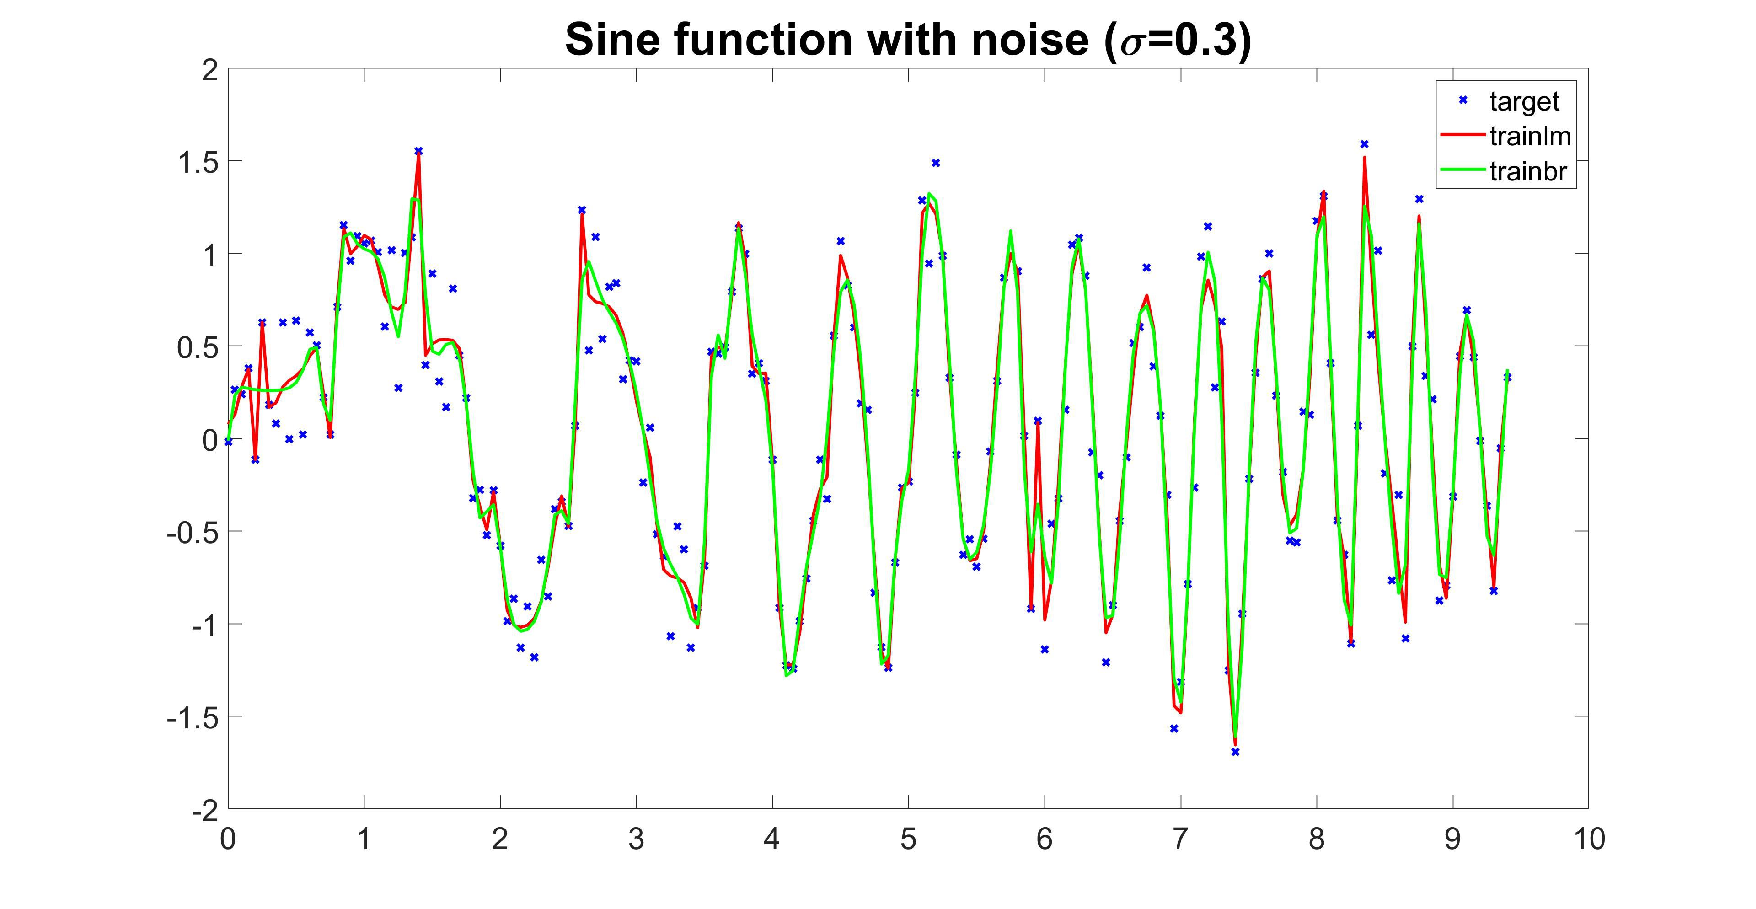
\includegraphics[width=\textwidth]{lab1/noisetrainbr.pdf}
  \caption{Sine function approx. with noise (with trainbr)}
  \label{fig:trainbrsinenoisecurve}
\end{figure}

In conclusion, most of the algorithms get affected by the number of training samples and neurons in each hidden layer. \verb|trainbr| has an advantage on overparametrised networks and prevents over-fitting; it also does not get influenced by the number of training samples much either. Generally, \verb|trainlm| is able to surpass most of the other algorithms but requires a significantly more memory use than the others. \verb|traingd| usually performs the weakest while the others such as \verb|trainbfg| and \verb|traincgp(f)| could have similar performances.


\section{Recurrent neural networks}

\subsection{Hopfield Network}

\subsubsection{2D Hopfield}
Hopfield neural network is a recurrent neural network, invented by John Hopfield in 1982. Hopfield network is a neural network combining storage system and binary system. 

In this case, we create a Hopfield network with three attractors (stable equilibrium points):

$\mathrm{T}=[1\;1;-1\;-1; 1\;-1]^{\mathrm{T}}$. We here define several random starting point and simulate the Hopfield network for 50 steps. Every point should reach one of the attractors. The result is shown below as Figure \ref{fig:similationhop1}.

\begin{figure}[h!]
  \centering
  % include second image
  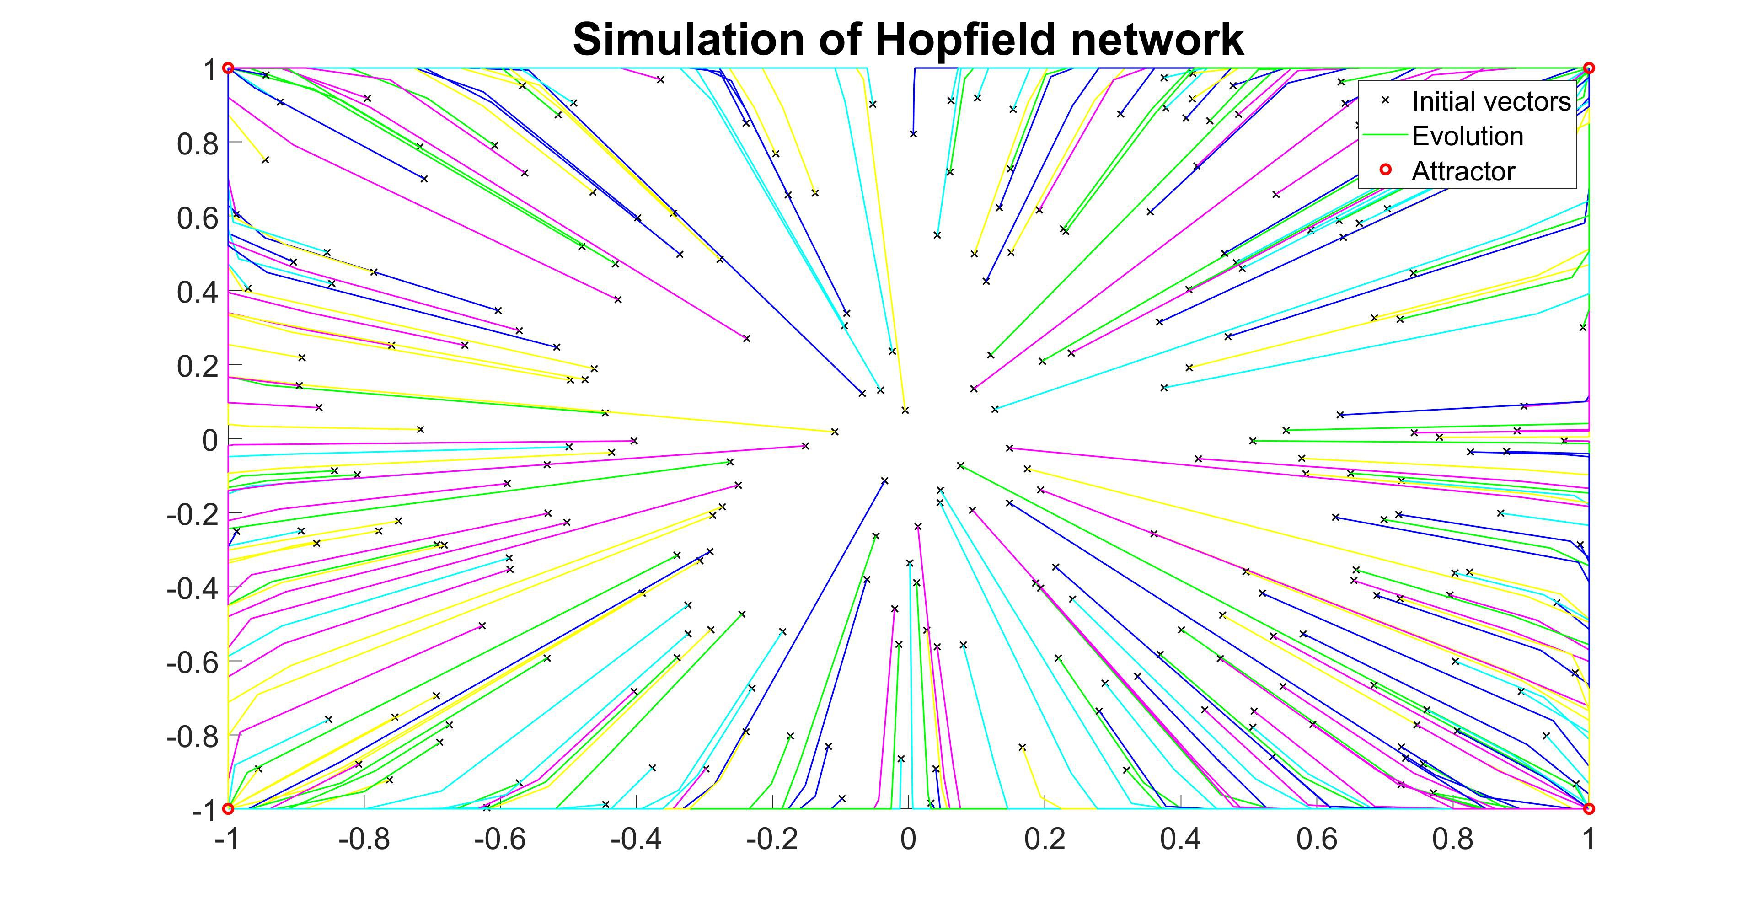
\includegraphics[width=\textwidth]{lab2/simulation1.pdf}
  \caption{Sample simulation of Hopfield network}
  \label{fig:similationhop1}
\end{figure}

We calculated out that the average iterations for random points take to reach attractors is around 11. This is averaged because the closer a point to one of the attractors, the faster it can reach the convergence. Here there is one more attractors than we specified, in the beginning, $[-1\;\;1]$ and also one unstable equilibrium point $[0\;\;0]$. We know that Hopfield network guarantees convergence to a local minimum, but it may also converge to the wrong local minimum, rather than the global minimum. Next, we are going to start from some special points, like those are parallel to $x$ or $y$-axis or on the diagonals. Figure \ref{fig:hop2d} gives us an illustration on how the evolution of these points running under Hopfield network and Figure \ref{fig:2dcombined} demonstrates a combined view of these particular points and those random points - proved that the real attractors are more than 3.


\begin{figure}[h!]
\begin{subfigure}[b]{.49\textwidth}
  \centering
  % include first image
  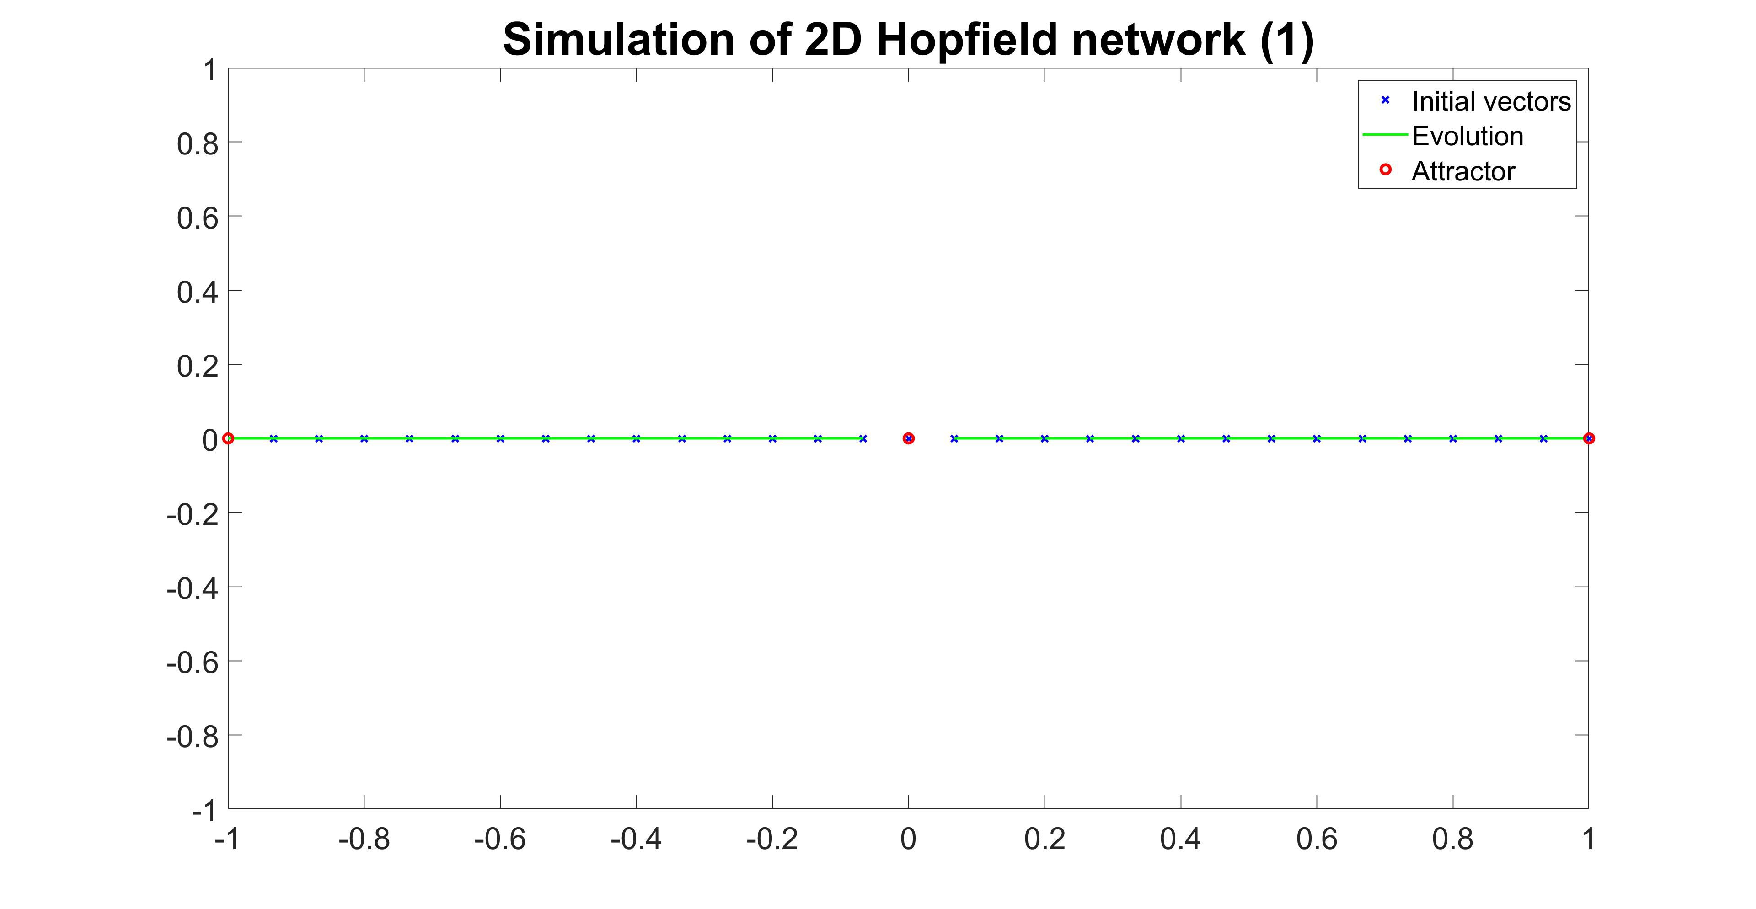
\includegraphics[width=\linewidth]{lab2/2d1.pdf}
  \caption{Points parallel to x-axis}
  \label{fig:xaxia}
\end{subfigure}
\hfill
\begin{subfigure}[b]{.49\textwidth}
  \centering
  % include first image
  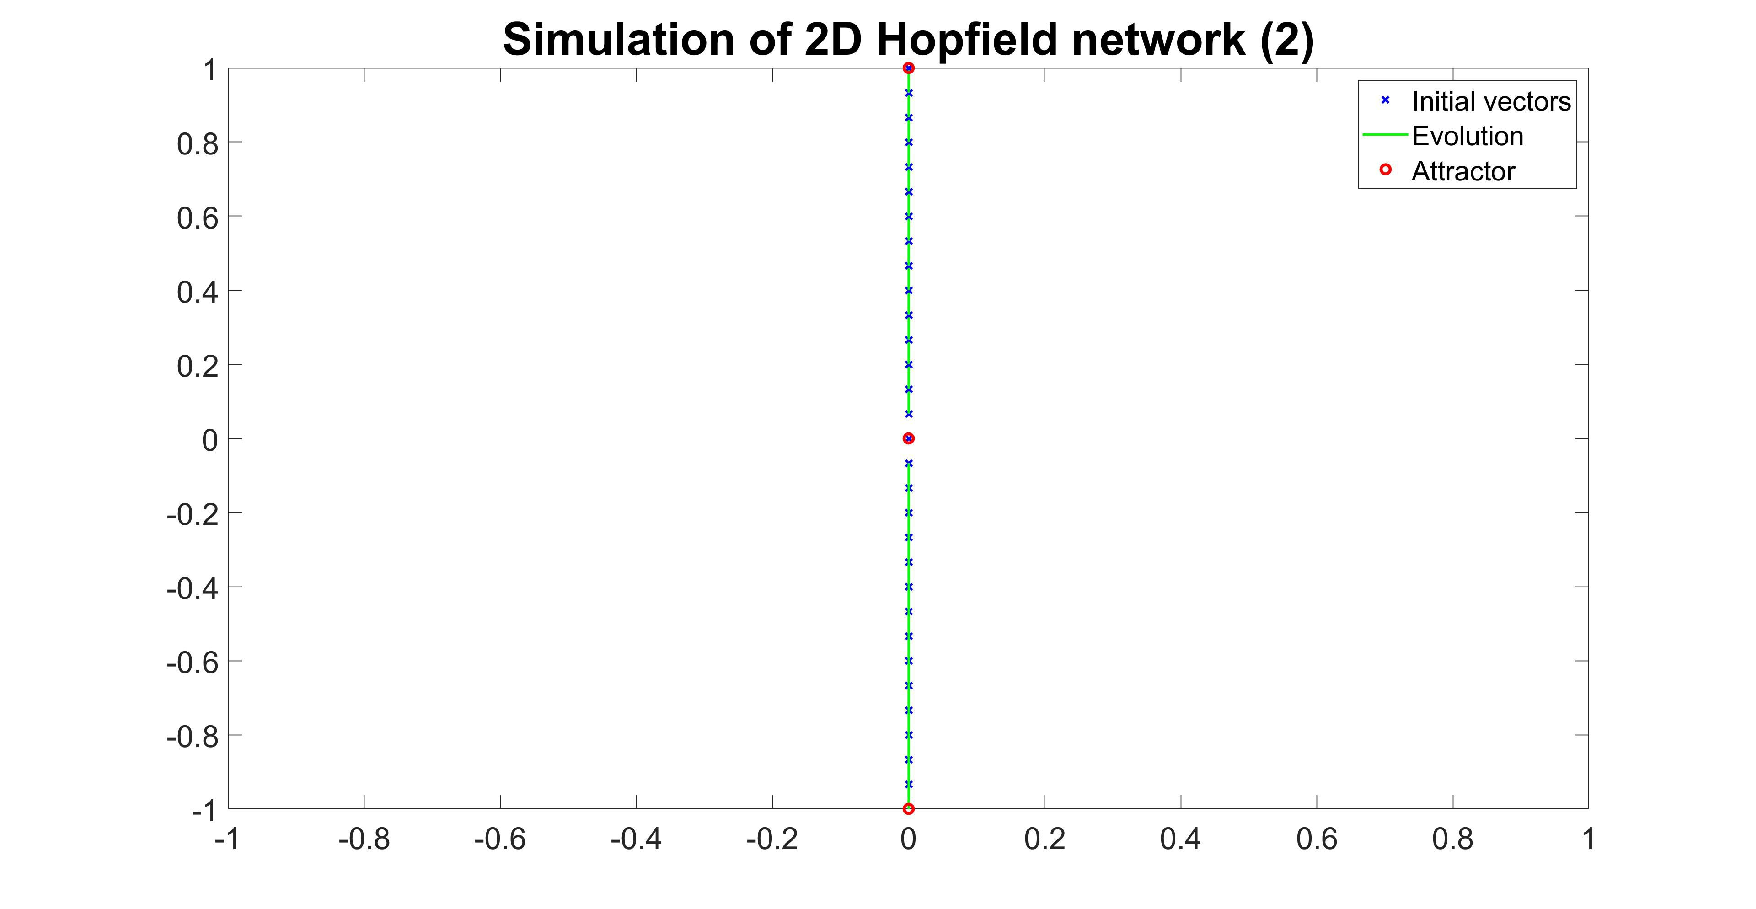
\includegraphics[width=\linewidth]{lab2/2d2.pdf}
  \caption{Points parallel to y-axis}
  \label{fig:yaxis}
\end{subfigure}


\begin{subfigure}[b]{.49\textwidth}
  \centering
  % include first image
  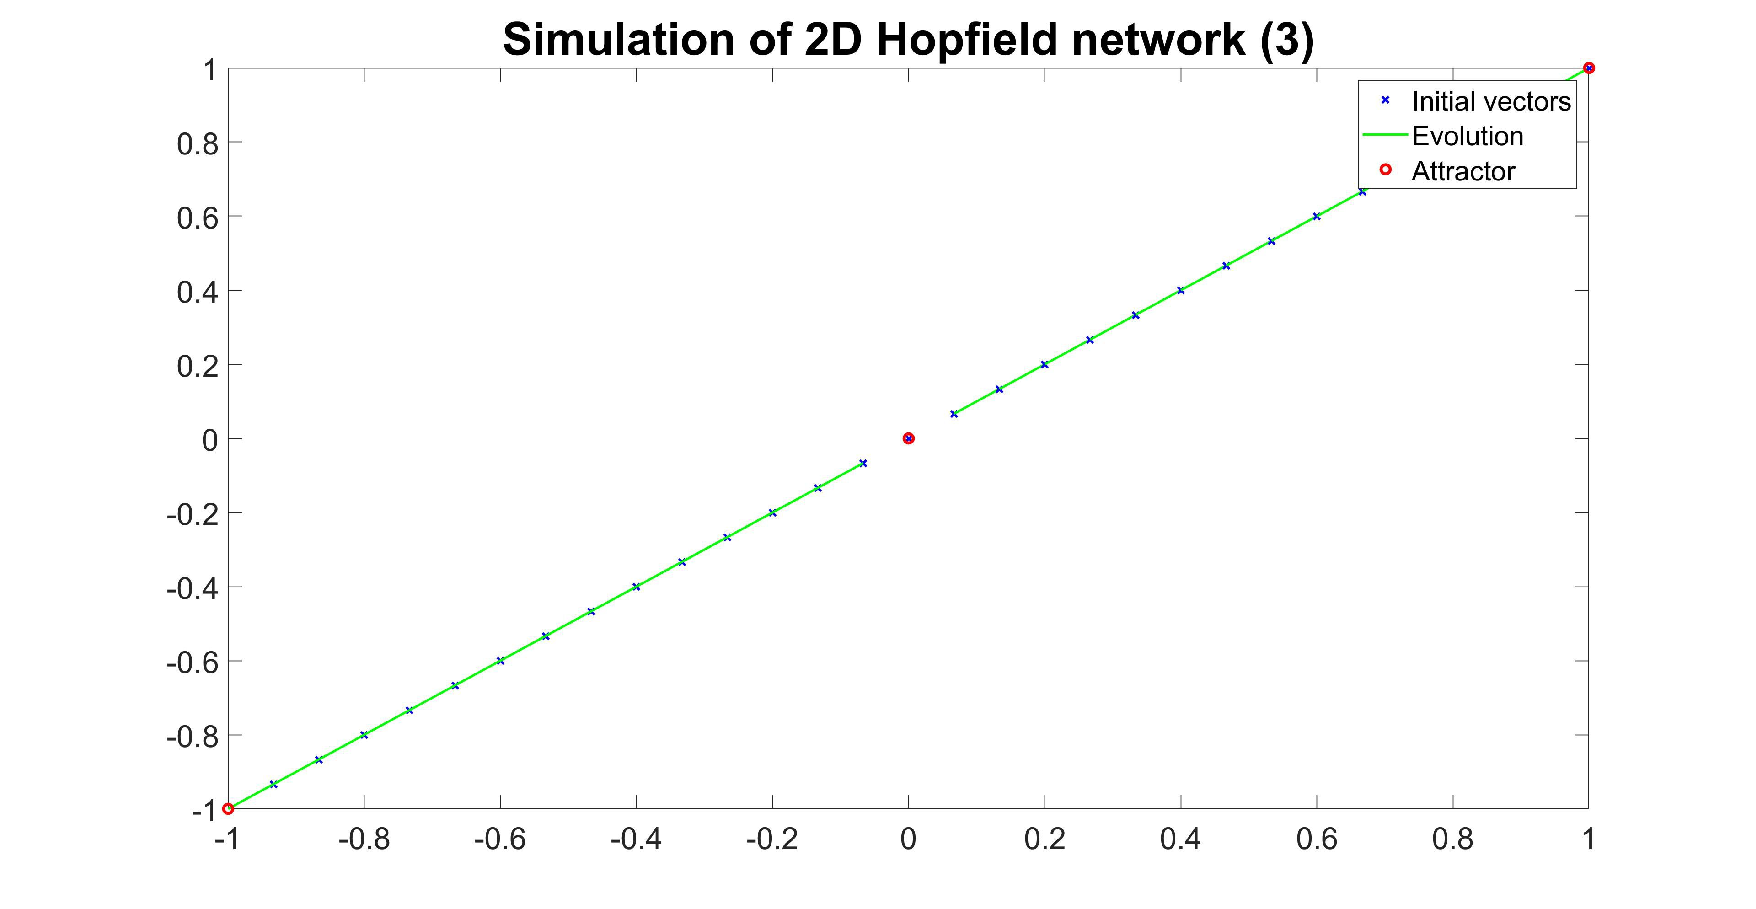
\includegraphics[width=\linewidth]{lab2/2d3.pdf}
  \caption{Diagonal points (positive slope)}
  \label{fig:diagpos}
\end{subfigure}
\hfill
\begin{subfigure}[b]{.49\textwidth}
  \centering
  % include first image
  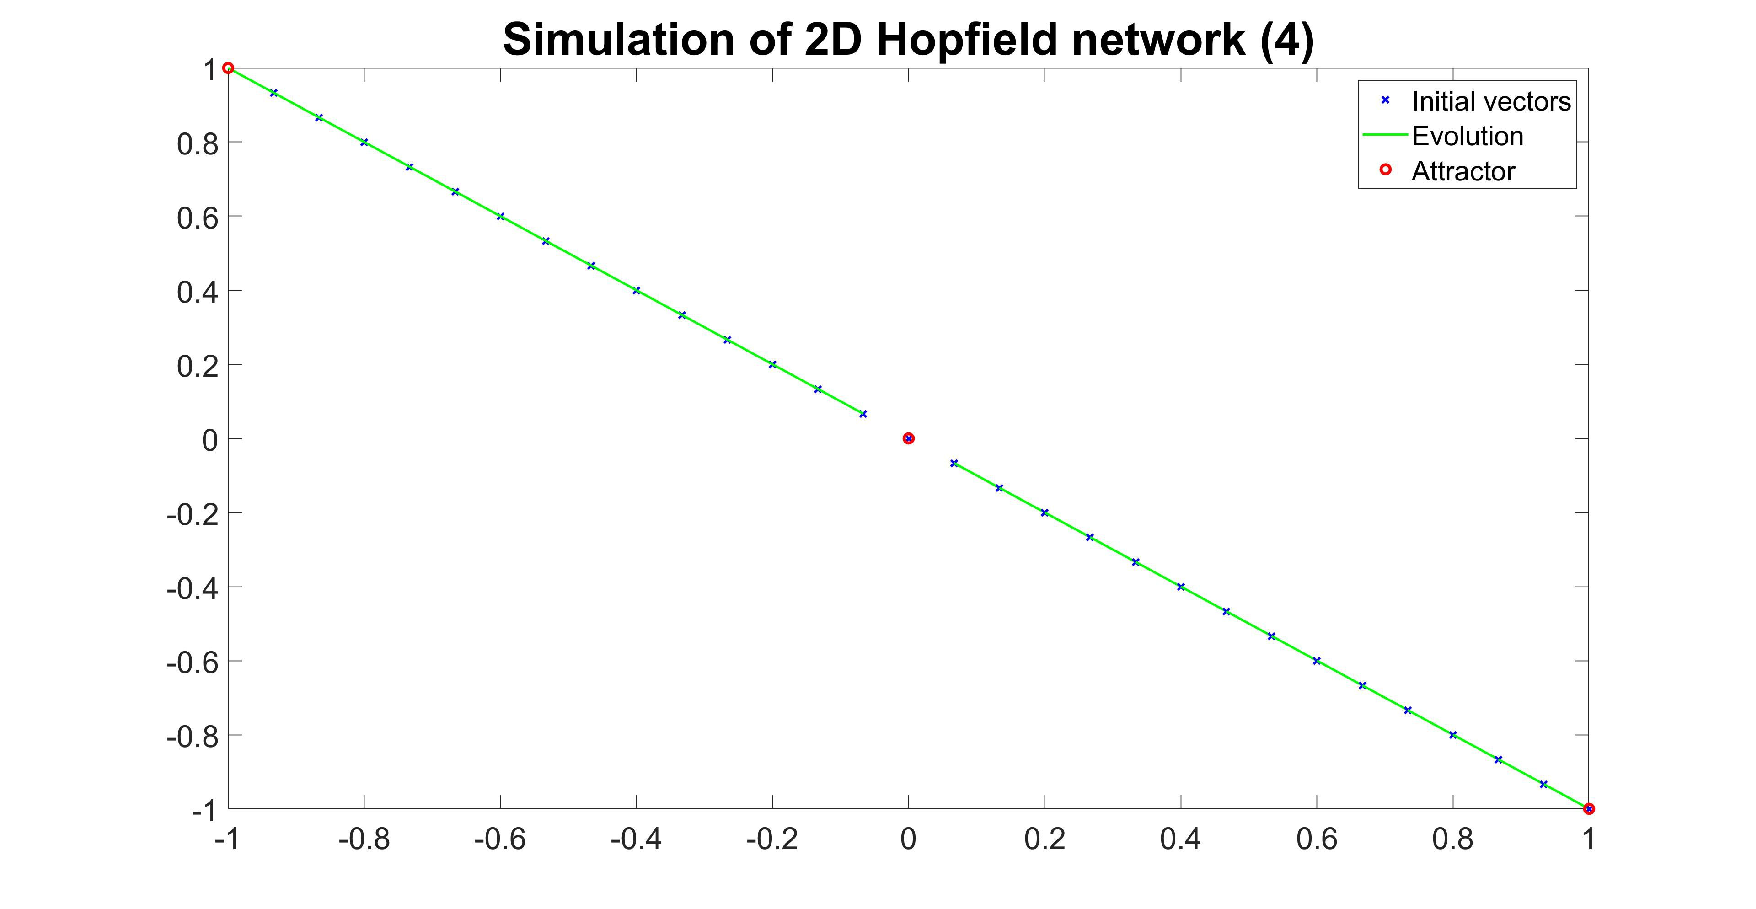
\includegraphics[width=\linewidth]{lab2/2d4.pdf}
  \caption{Diagonal points (negative slope)}
  \label{fig:diagneg}
\end{subfigure}
\caption{Special starting point on 2D Hopfield network}
\label{fig:hop2d}
\end{figure}


\subsubsection{3D Hopfield}

Now we try the 3D Hopfield network. Because of the extra dimension, we noticed a slightly increased average iteration to reach attractors: around 14 iterations. It is interesting to see that the attractors changed in this case, which is no longer the stable four we mentioned in prior. This may be caused by the increasing uncertainty brought by the extra neuron. But the unstable equilibrium we mentioned above still exists in this case which locates in the centre of our plot. 


\begin{figure}[h!]
\begin{subfigure}[b]{.49\textwidth}
  \centering
  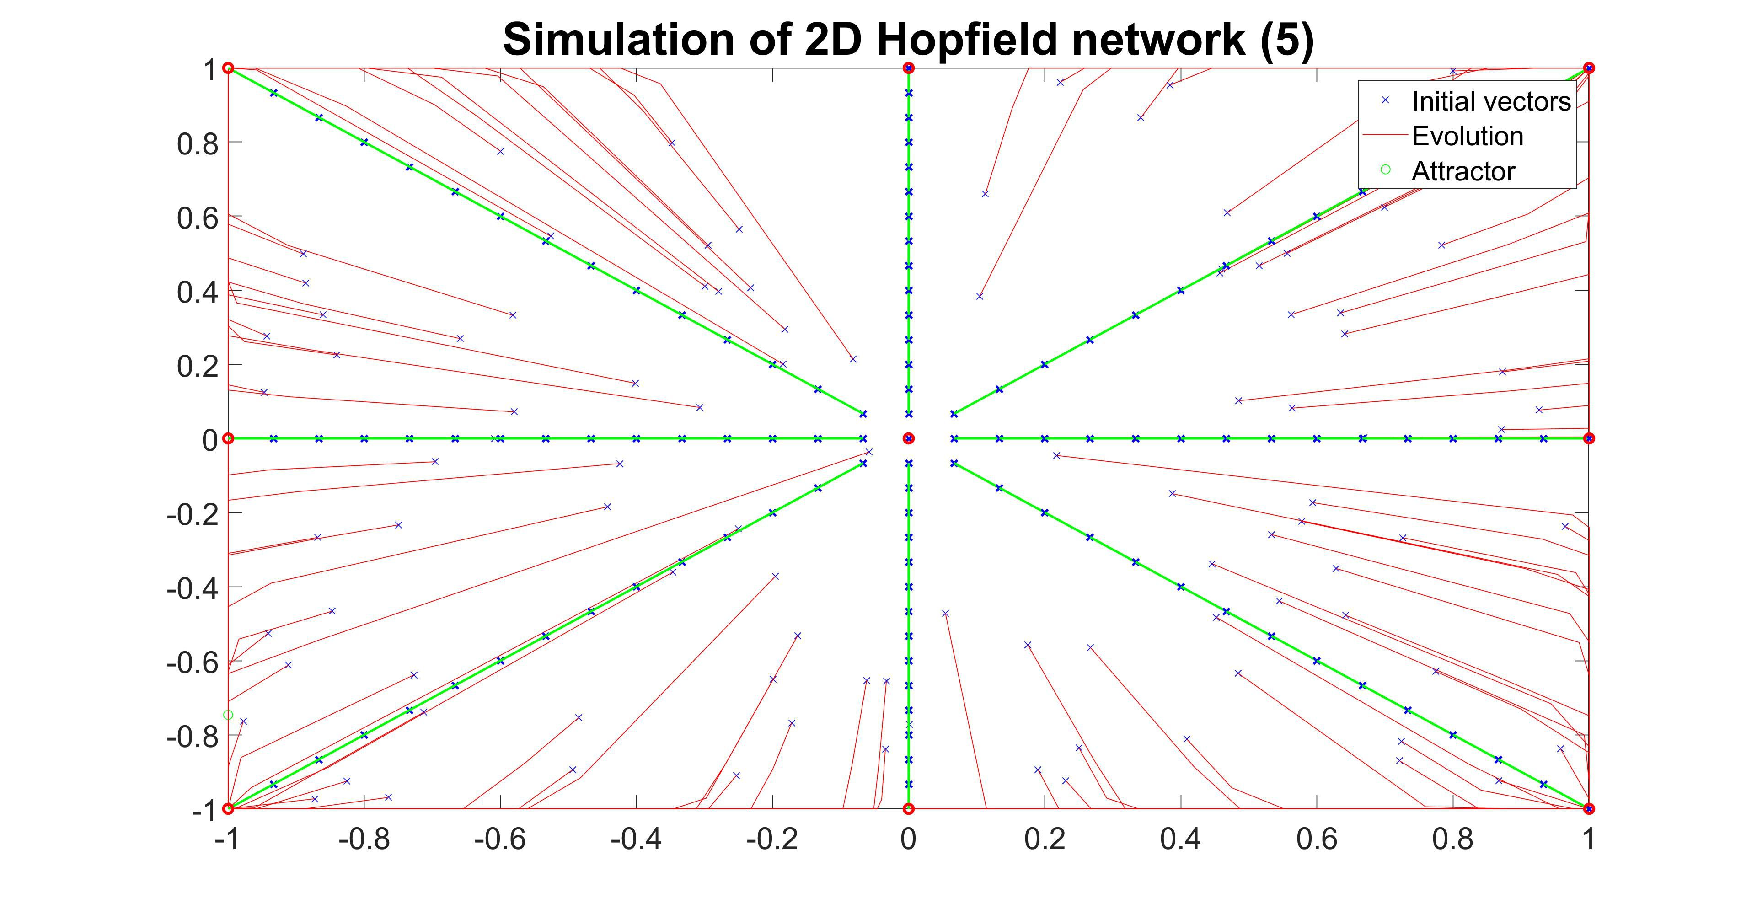
\includegraphics[width=\linewidth]{lab2/2d5.pdf}
  \caption{Combined starting points on 2D Hopfield}
  \label{fig:2dcombined}
\end{subfigure}
\hfill
\begin{subfigure}[b]{.49\textwidth}
  \centering
  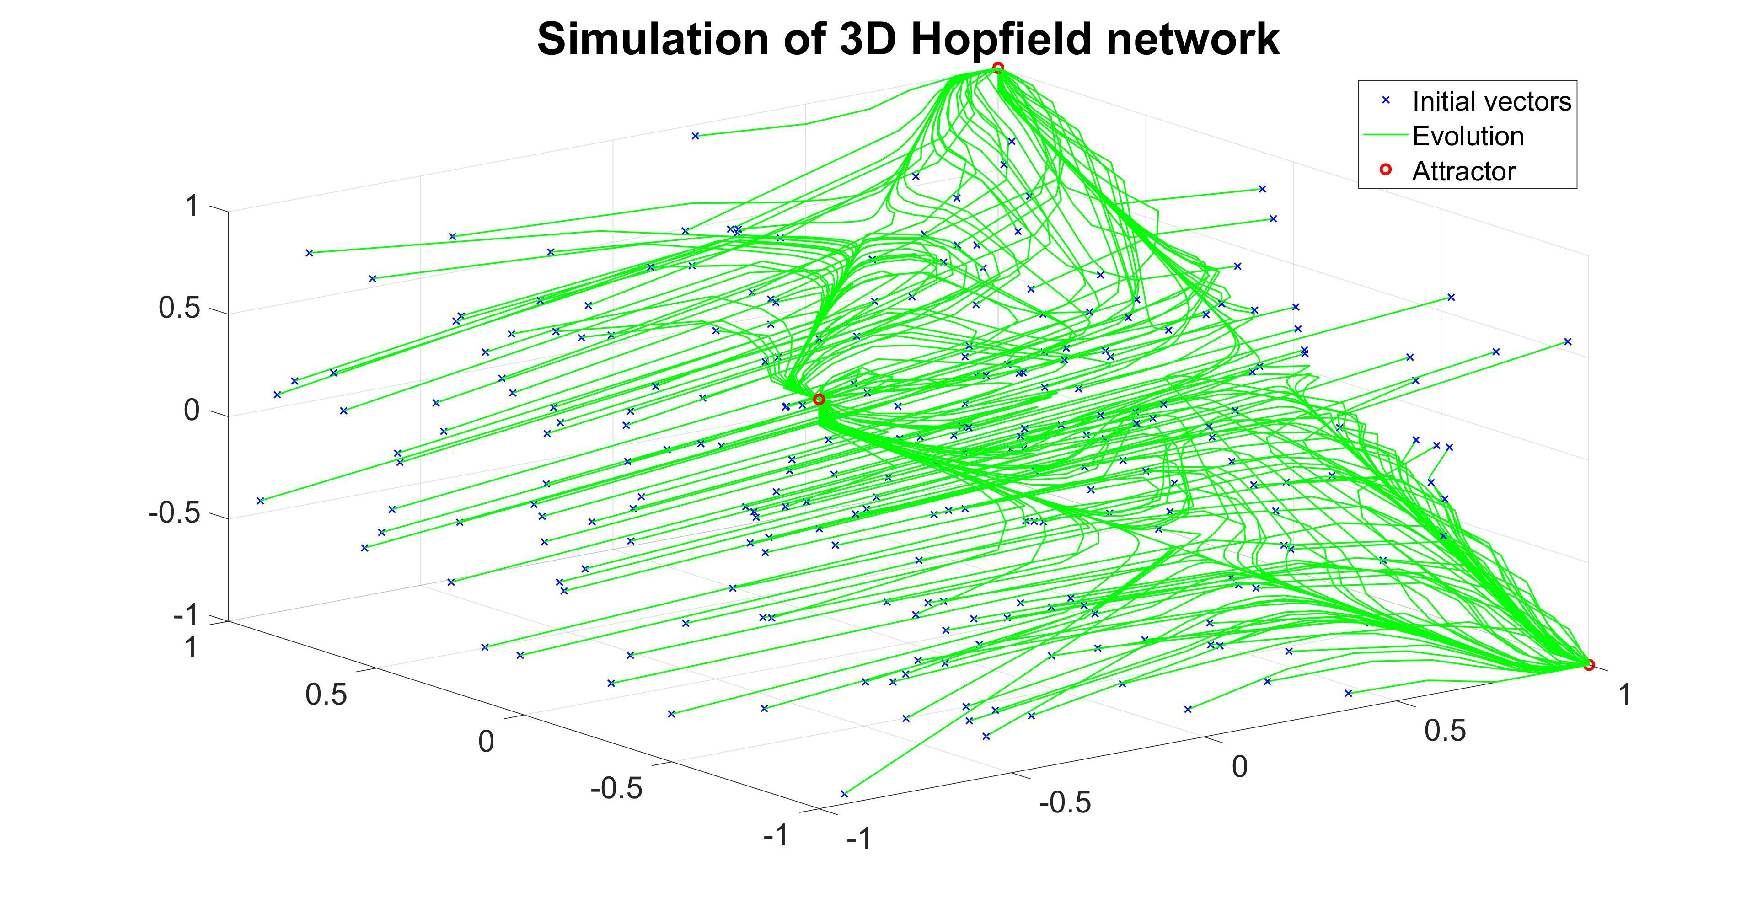
\includegraphics[width=\linewidth]{lab2/3d.pdf}
  \caption{Performance comparison with noise (neuron=70)}
  \label{fig:3dhop}
\end{subfigure}
\caption{Simulations of Hopfield network}
\label{fig:fig}
\end{figure}

\subsubsection{Pattern retrieval}

As in the assignment description: ``the function \verb|hopdigit| creates a Hopfield network which has as attractors the handwritten digits 0, ..., 9.'' The task here is to check whether the Hopfield network has the ability to reconstruct the noisy digits. Here we tested the noisy level from 1 to 10 along with five levels of iterations: 10, 50, 100, 500, and 1000. 

Generally, the more noise added the more iterations required for Hopfield network to reconstruct it to the closest attractor as those noises push the initials away from attractors. However, when the noise level is too high ($\geq8$), it is possible for the Hopfield network to converge to a wrong attractor. In Figure \ref{fig:noise10ite500}, even though the iterations are high enough as 500, the reconstructed results for digits ``0, 2, 5, 6, 7'' were all wrong, for instance, digit ``2'' with too much noise could be simply transformed to be more ``close'' to another attractor digit ``7''. Rather than these existing attractors, without enough iterations, the final result could lead to spurious attractors. Figure \ref{fig:hopnoise1}, \ref{fig:hopnoise5} and \ref{fig:hopnoise10} show the results under different combinations of noise levels and iteration numbers.

\begin{figure}[h!]
     \centering
     \begin{subfigure}[b]{0.3\textwidth}
         \centering
         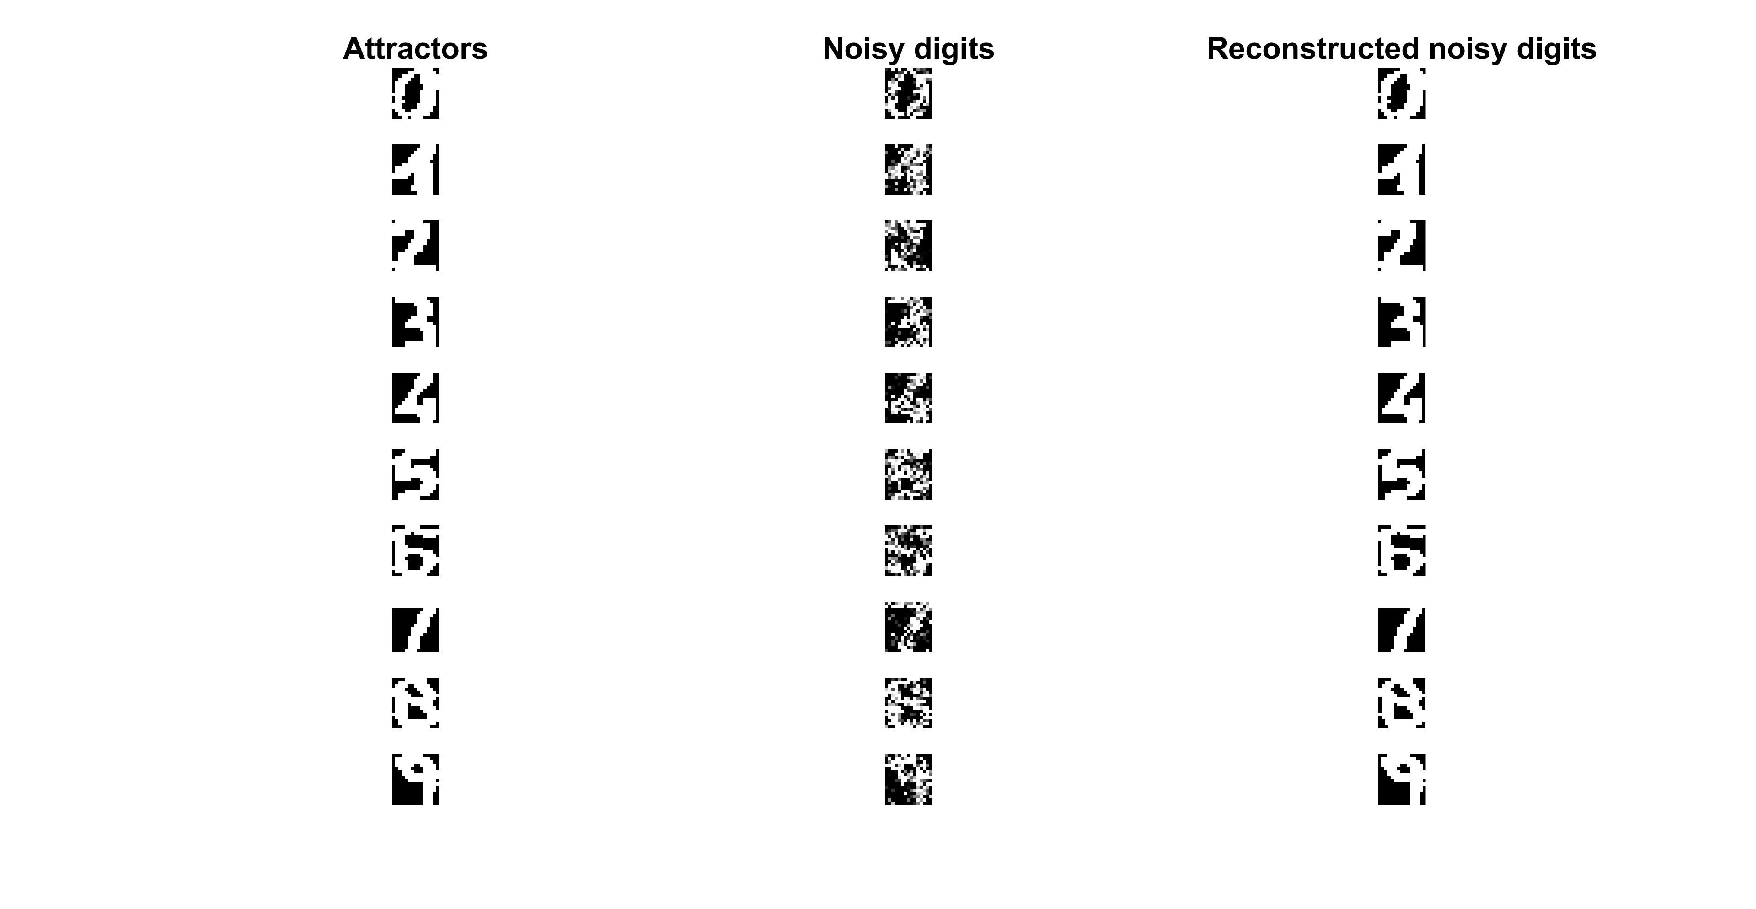
\includegraphics[width=\textwidth]{lab2/noise1ite10.pdf}
         \caption{Noise=1, iteration=10}
         \label{fig:noise1ite10}
     \end{subfigure}
     \hfill
     \begin{subfigure}[b]{0.3\textwidth}
         \centering
         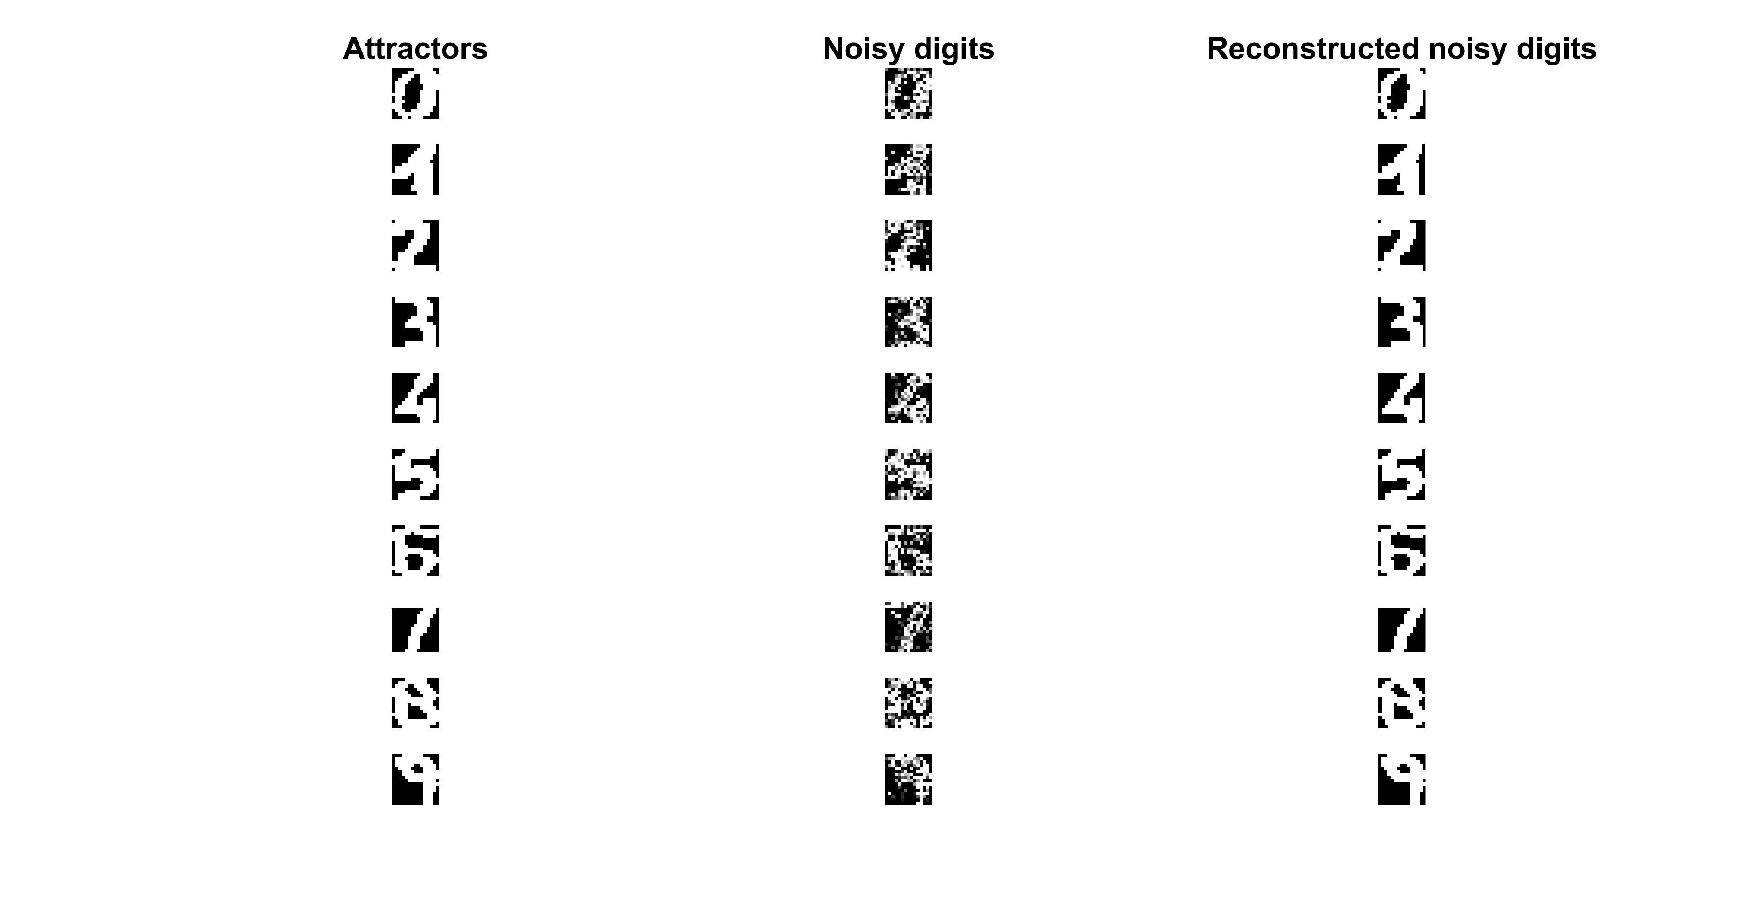
\includegraphics[width=\textwidth]{lab2/noise1ite100.pdf}
         \caption{Noise=1, iteration=100}
         \label{fig:noise1ite100}
     \end{subfigure}
     \hfill
     \begin{subfigure}[b]{0.3\textwidth}
         \centering
         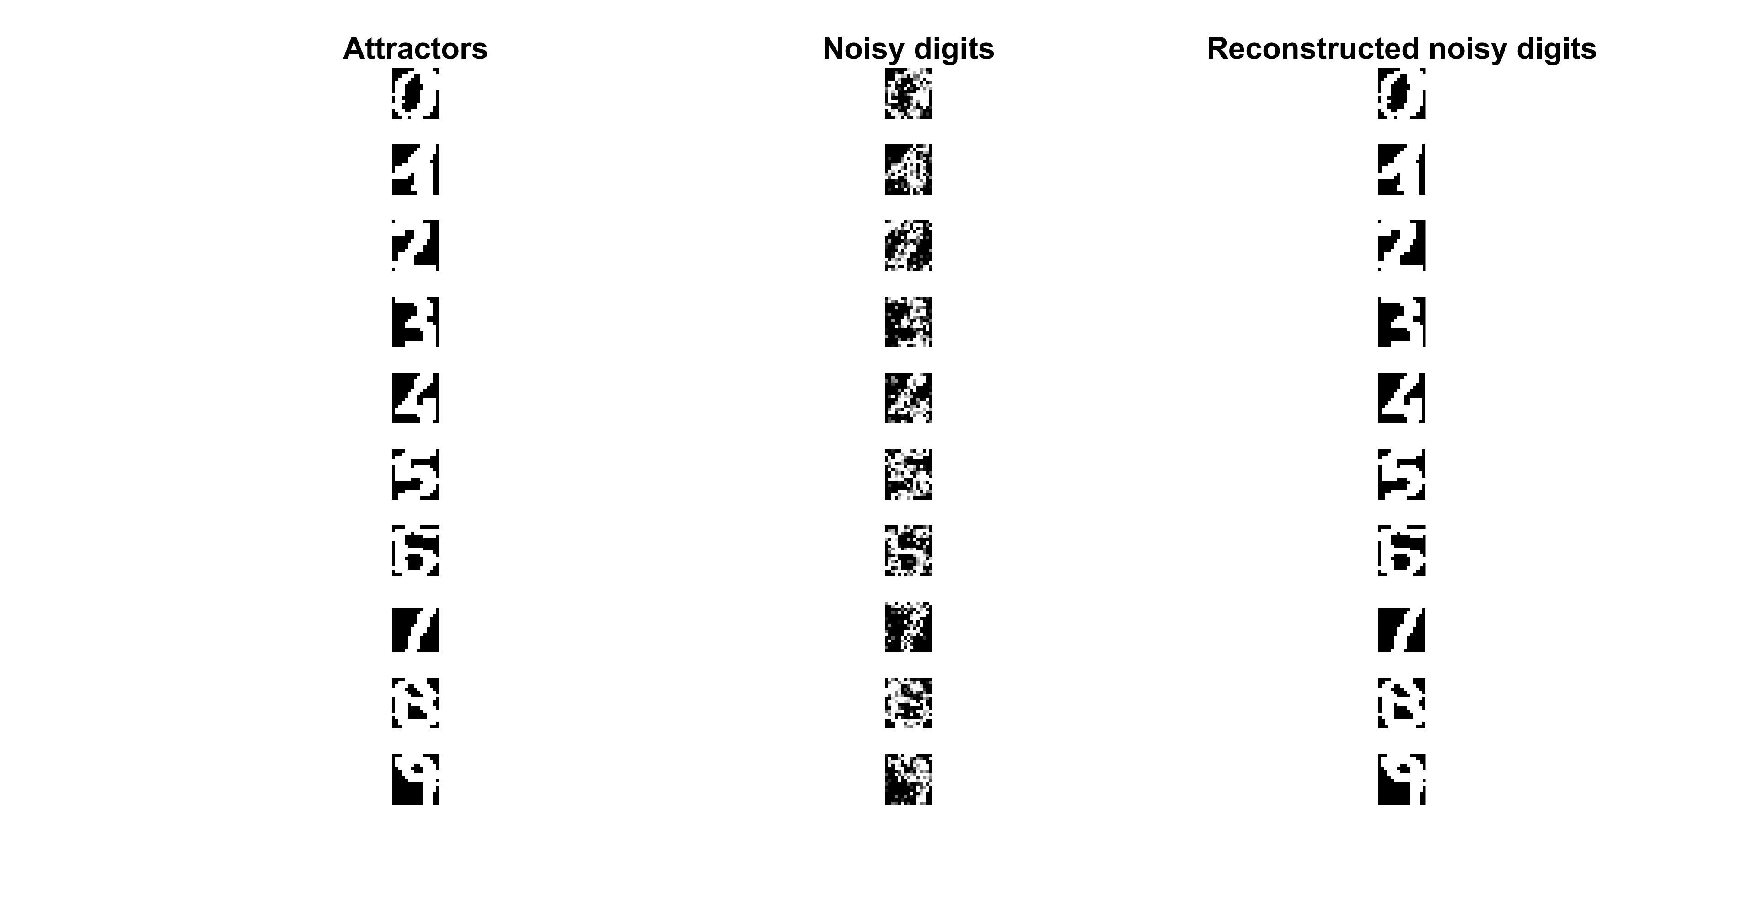
\includegraphics[width=\textwidth]{lab2/noise1ite500.pdf}
         \caption{Noise=1, iteration=500}
         \label{fig:noise1ite500}
     \end{subfigure}
        \caption{Noise=1}
        \label{fig:hopnoise1}
\end{figure}

%%%%%%
\begin{figure}[h!]
     \centering
     \begin{subfigure}[b]{0.3\textwidth}
         \centering
         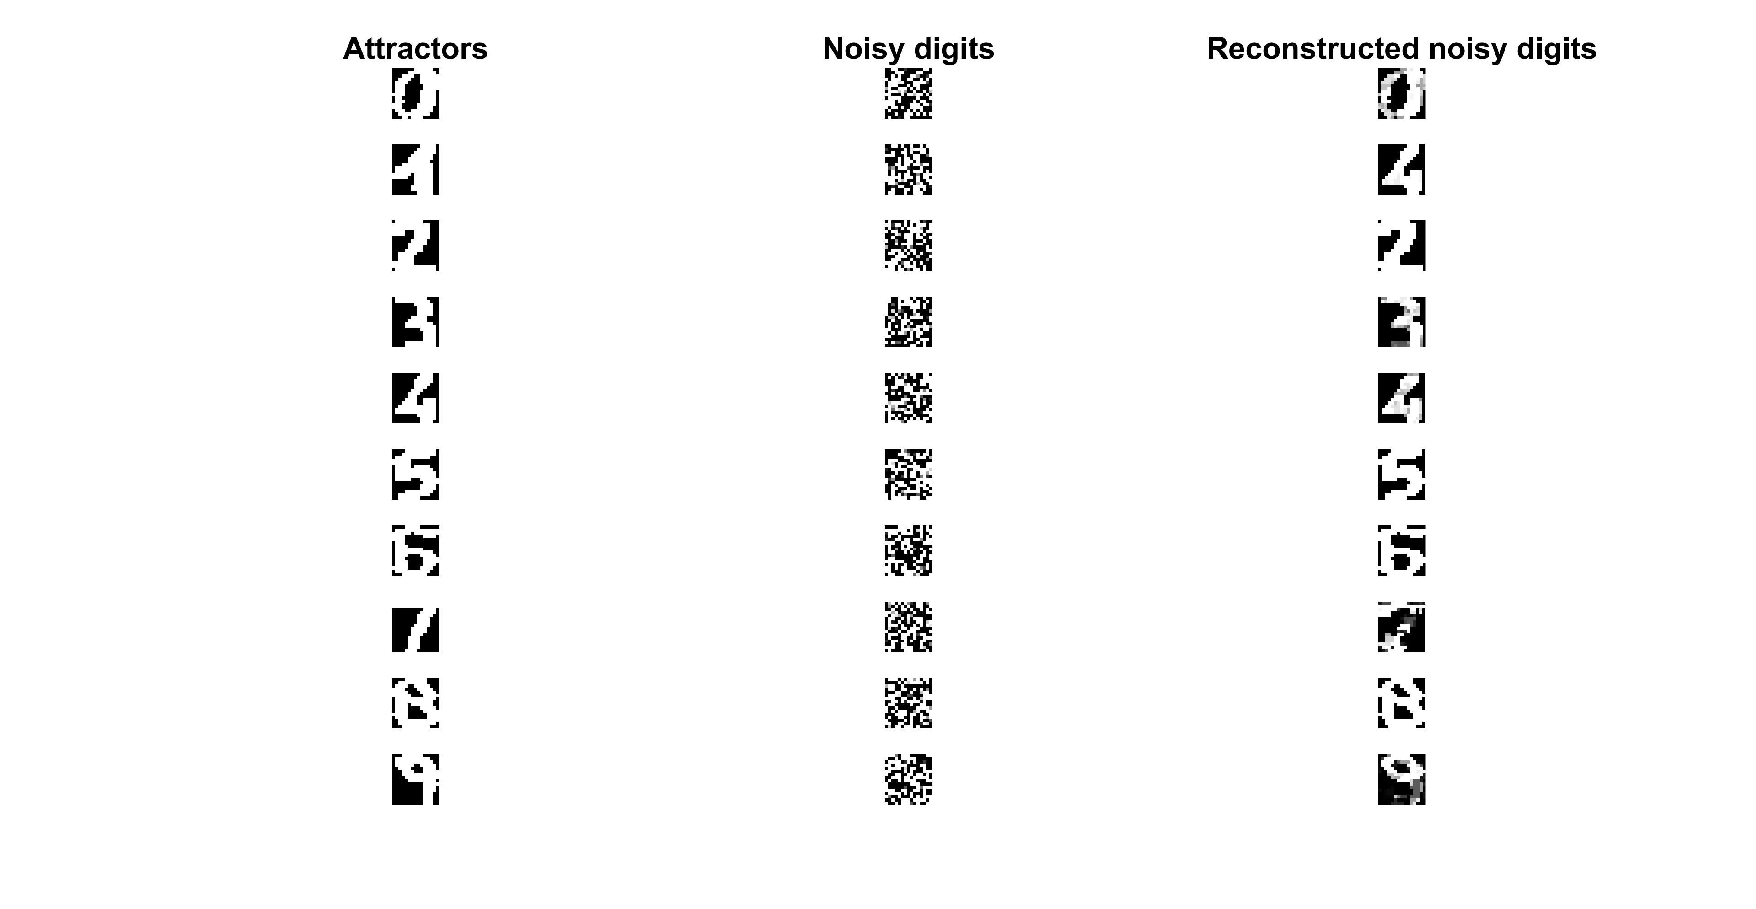
\includegraphics[width=\textwidth]{lab2/noise5ite10.pdf}
         \caption{Noise=5, iteration=10}
         \label{fig:noise5ite10}
     \end{subfigure}
     \hfill
     \begin{subfigure}[b]{0.3\textwidth}
         \centering
         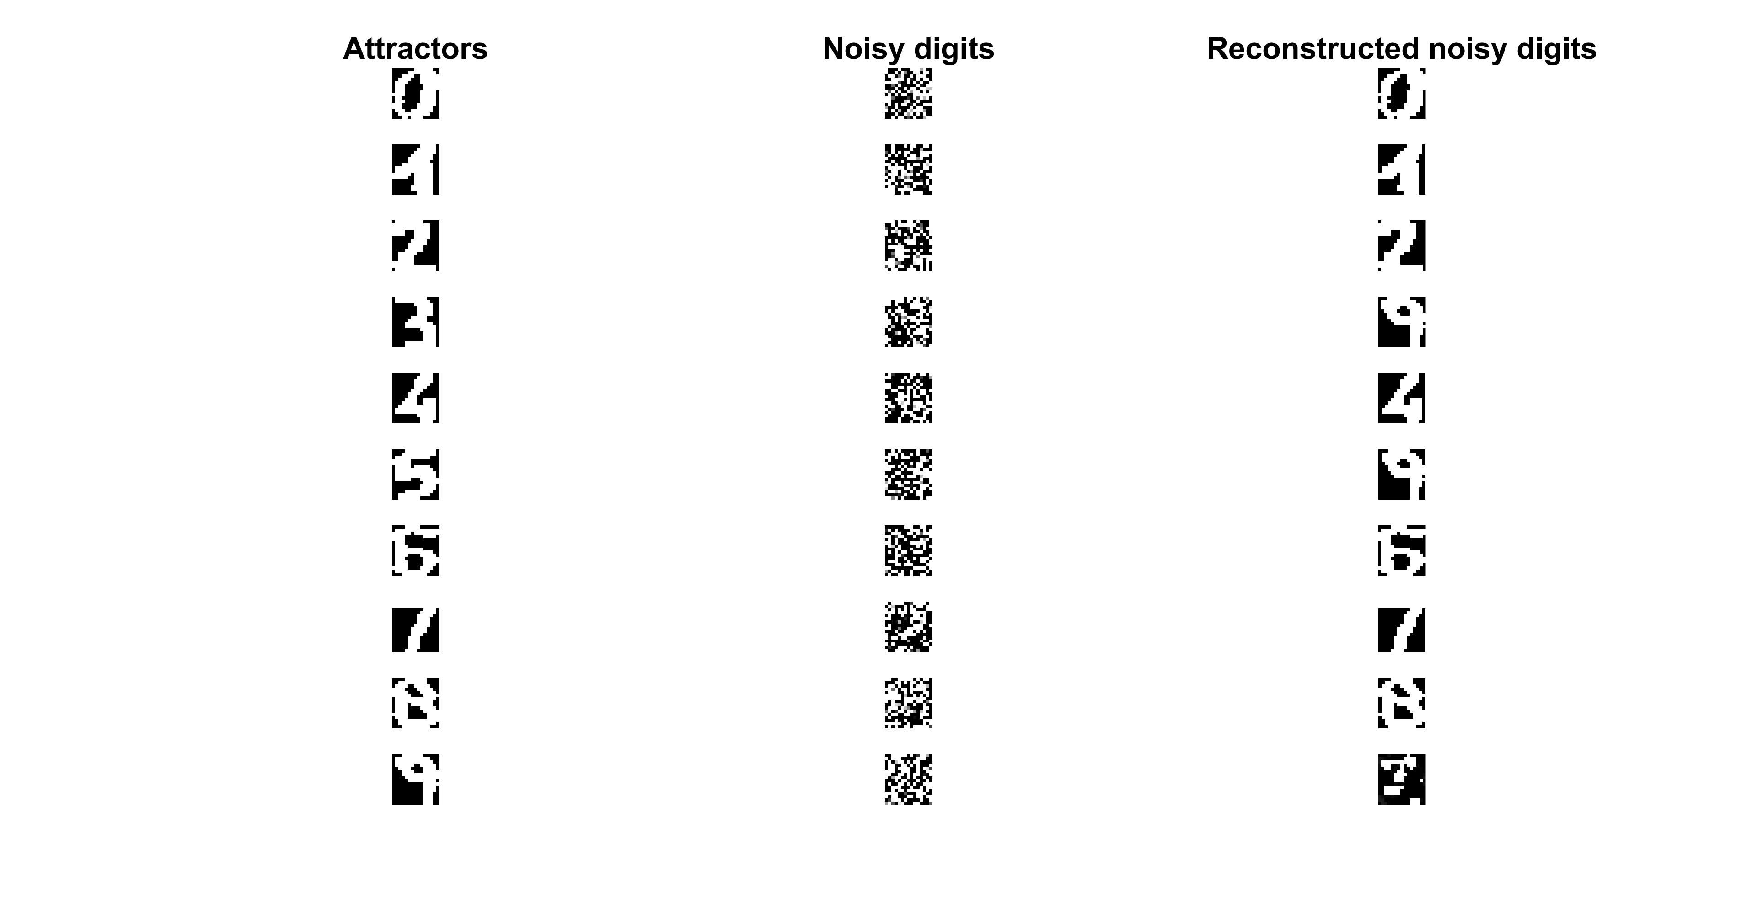
\includegraphics[width=\textwidth]{lab2/noise5ite100.pdf}
         \caption{Noise=5, iteration=100}
         \label{fig:noise5ite100}
     \end{subfigure}
     \hfill
     \begin{subfigure}[b]{0.3\textwidth}
         \centering
         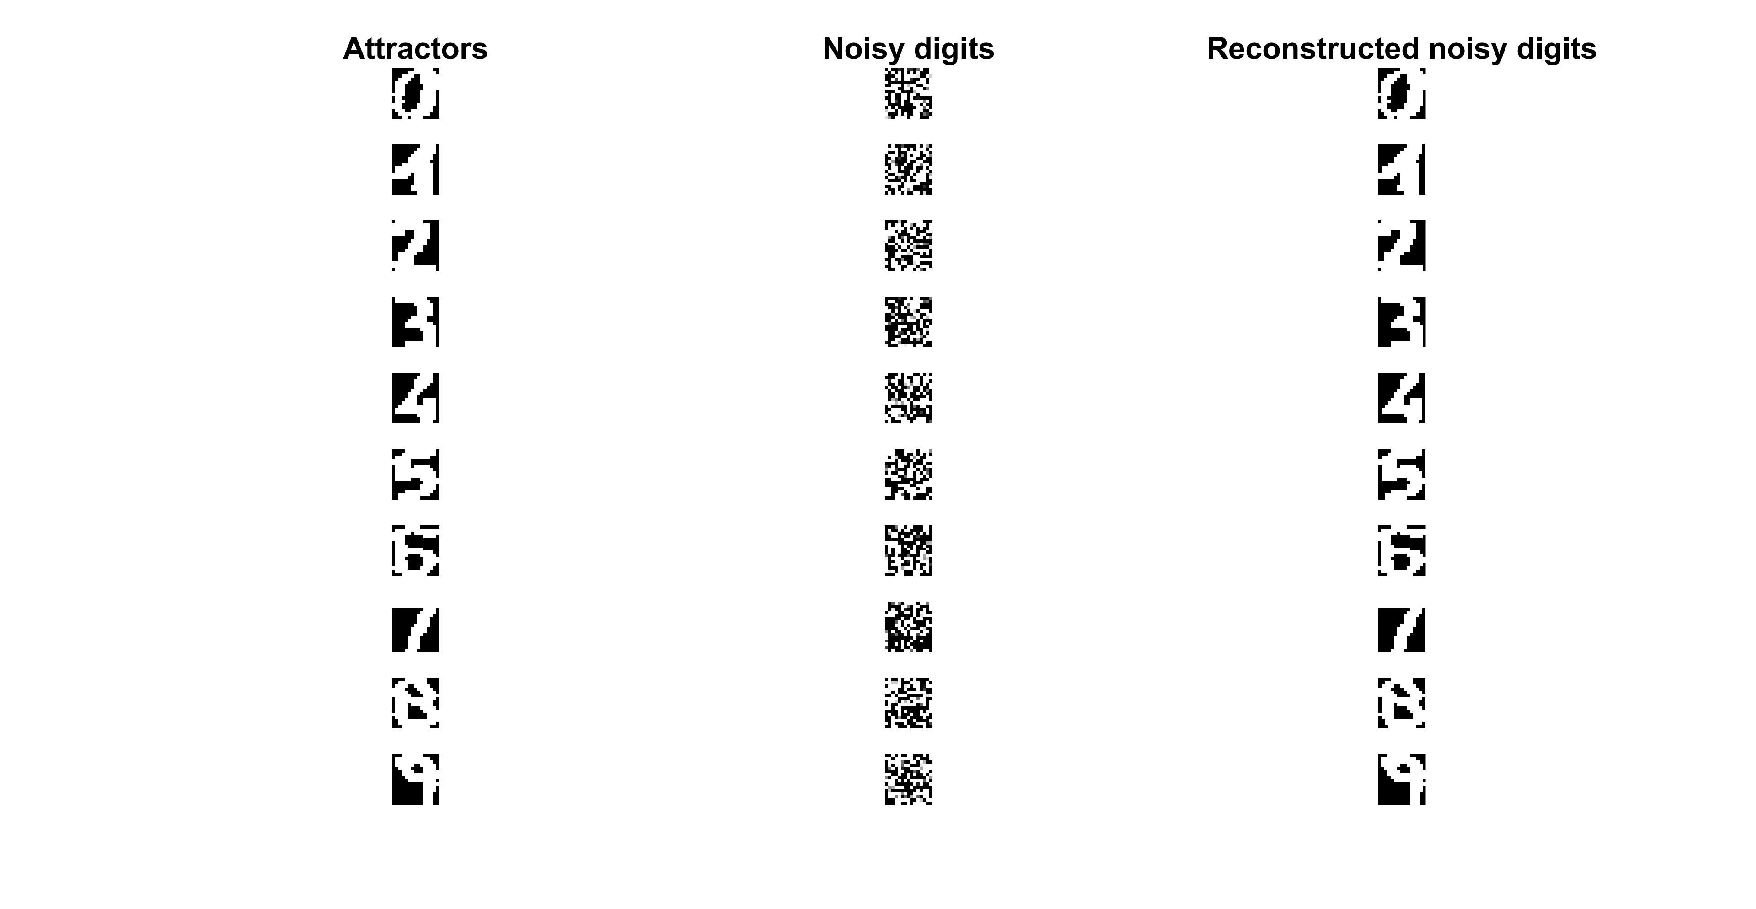
\includegraphics[width=\textwidth]{lab2/noise5ite500.pdf}
         \caption{Noise=5, iteration=500}
         \label{fig:noise5ite500}
     \end{subfigure}
        \caption{Noise=5}
        \label{fig:hopnoise5}
\end{figure}

%%%%%
\begin{figure}[h!]
     \centering
     \begin{subfigure}[b]{0.3\textwidth}
         \centering
         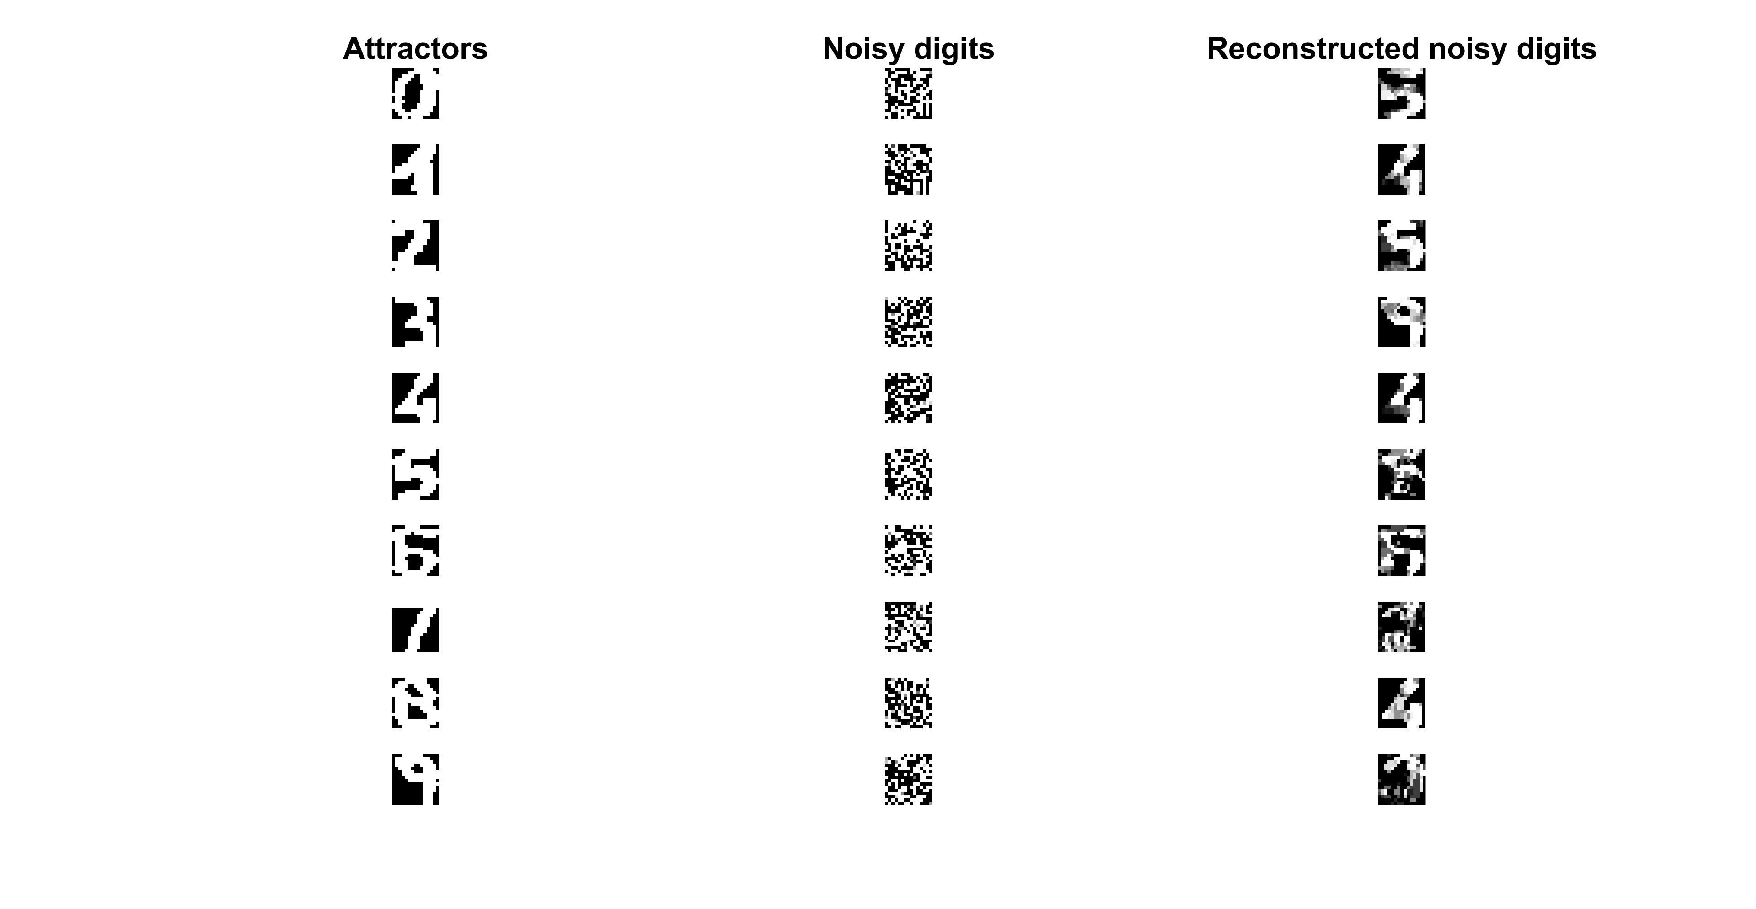
\includegraphics[width=\textwidth]{lab2/noise10ite10.pdf}
         \caption{Noise=10, iteration=10}
         \label{fig:noise10ite10}
     \end{subfigure}
     \hfill
     \begin{subfigure}[b]{0.3\textwidth}
         \centering
         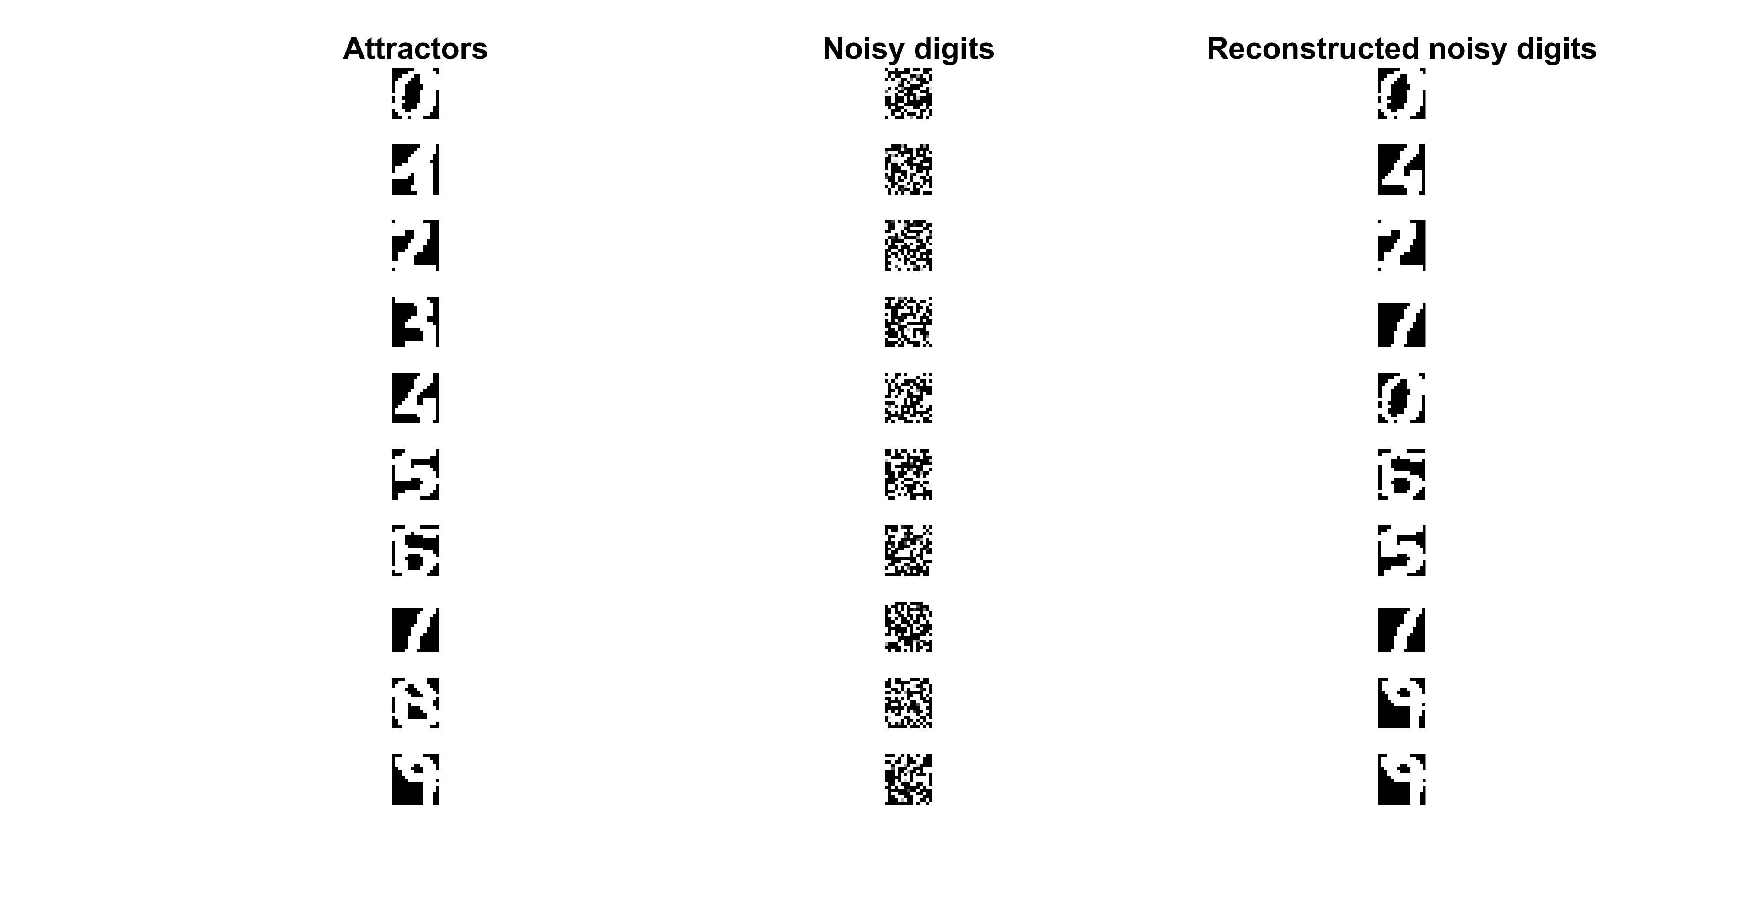
\includegraphics[width=\textwidth]{lab2/noise10ite100.pdf}
         \caption{Noise=10, iteration=100}
         \label{fig:noise10ite100}
     \end{subfigure}
     \hfill
     \begin{subfigure}[b]{0.3\textwidth}
         \centering
         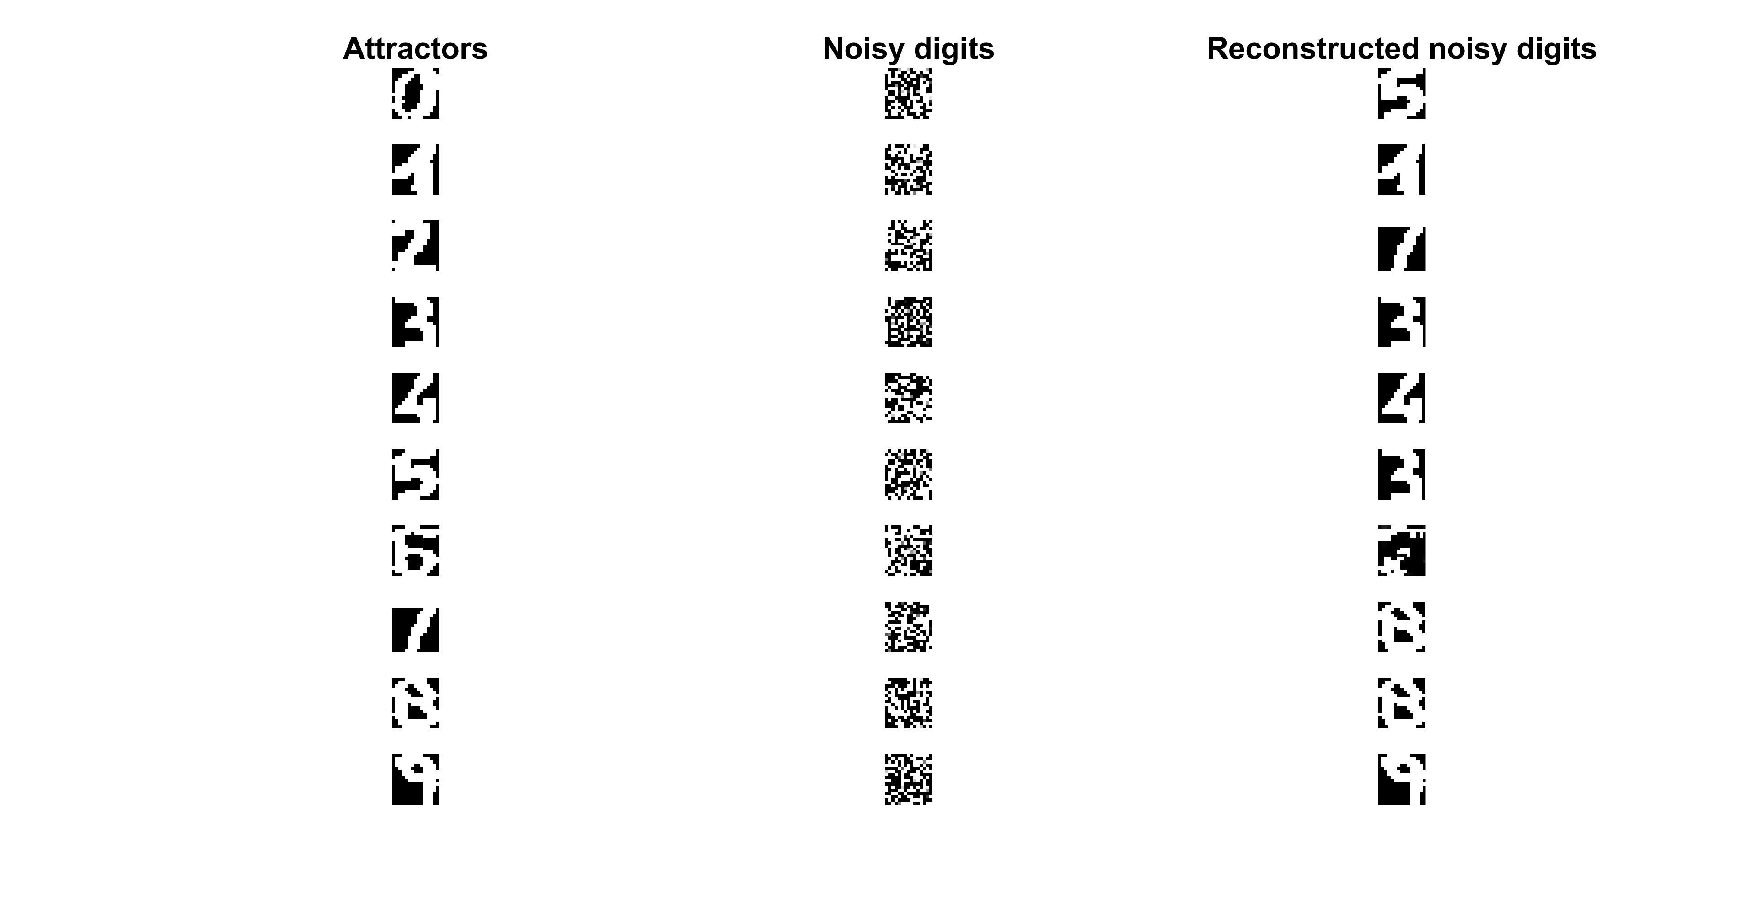
\includegraphics[width=\textwidth]{lab2/noise10ite500.pdf}
         \caption{Noise=10, iteration=500}
         \label{fig:noise10ite500}
     \end{subfigure}
        \caption{Noise=10}
        \label{fig:hopnoise10}
\end{figure}

We aimed to find a combination with the most noise but least number of iterations with perfect reconstruction result, it came out that noise level 4 only requires 15 iterations to reconstruct every digit. The result is shown in Figure \ref{fig:finalnoise}.

Overall, the Hopfield network is doing well for this task.

%%%%
\begin{figure}[h!]
  \centering
  % include second image
  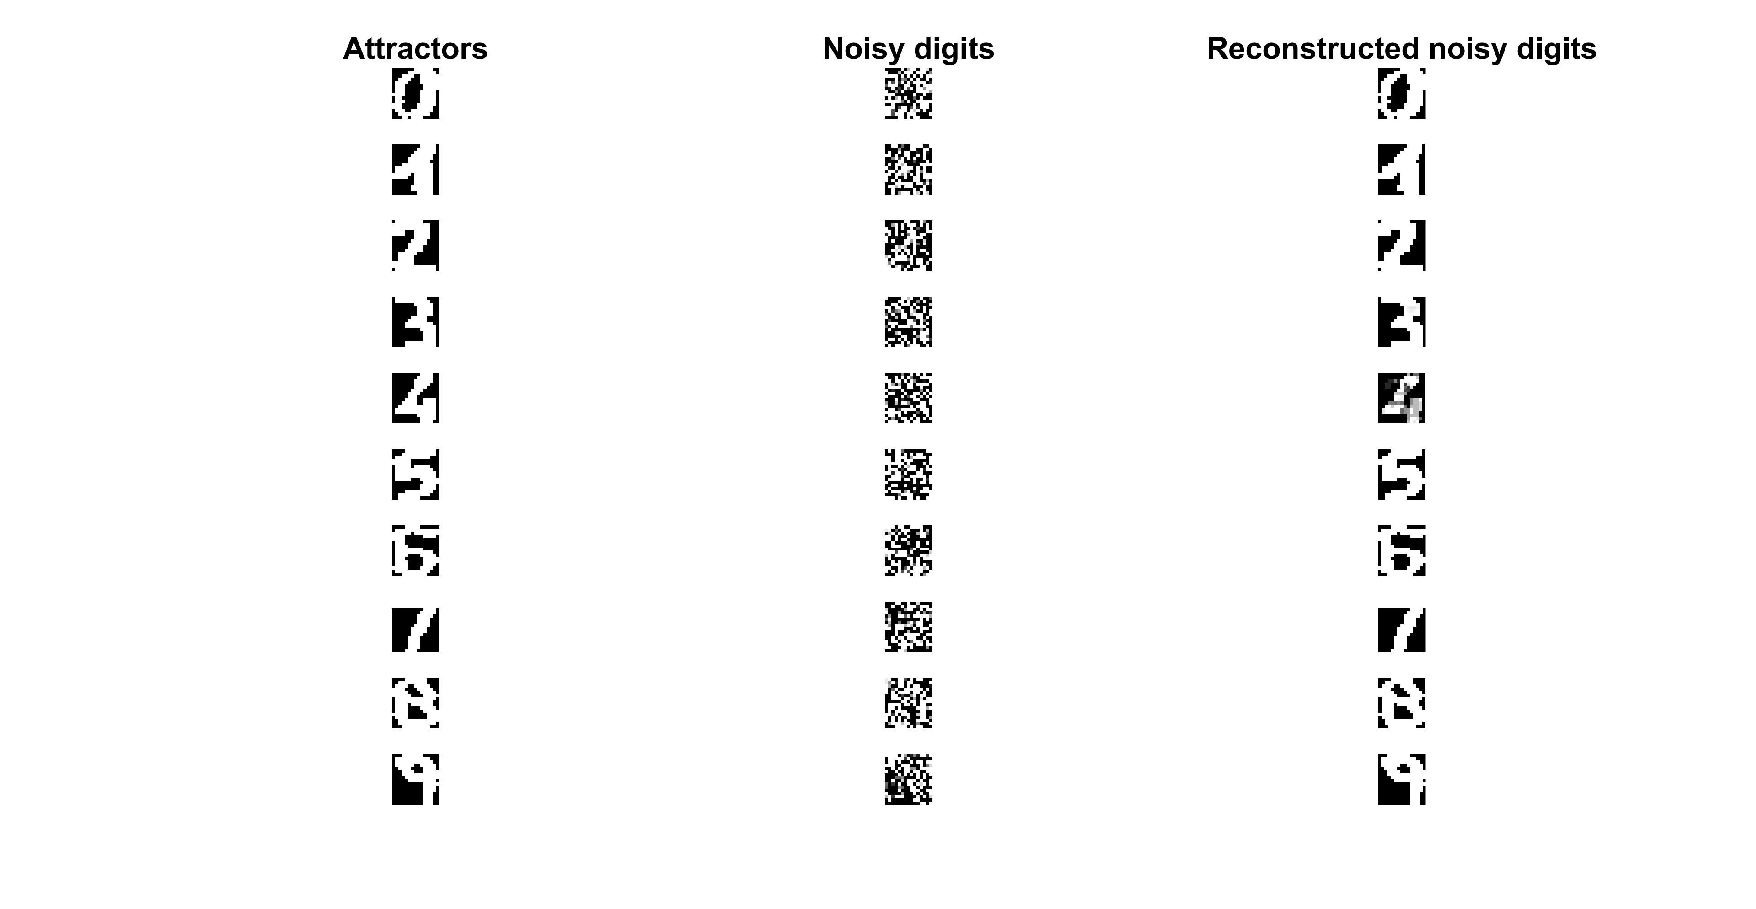
\includegraphics[width=.85\textwidth]{lab2/noise4ite15.pdf}
  \caption{Noise=4, iteration=15 (best result on max noise and min iteration)}
  \label{fig:finalnoise}
\end{figure}


\subsection{MLP for time series prediction}
In this section, we try to design and train an MLP with one hidden layer after standardising the data set. The dataset construction is done using \verb|getTimeSeriesTrainData| function, which brings two important parameters for this MLP model: numbers of hidden neurons in the hidden layer and the lag value. Here we tested several combinations of lag value (5 to 500 by 25) and hidden neuron amount (1 to 70 by 5), the average result looks not accuracy on predicting last 40 observations and normally have over 500 RMSE shown in Figure \ref{fig:mlpavg}. But there is a combination: lag value = 5 and hidden neuron = 13 produced promising result comparing to the others. Its result is demonstrated in Figure \ref{fig:nlpbest}.


\begin{figure}[h!]
\begin{subfigure}[b]{.49\textwidth}
  \centering
  % include first image
  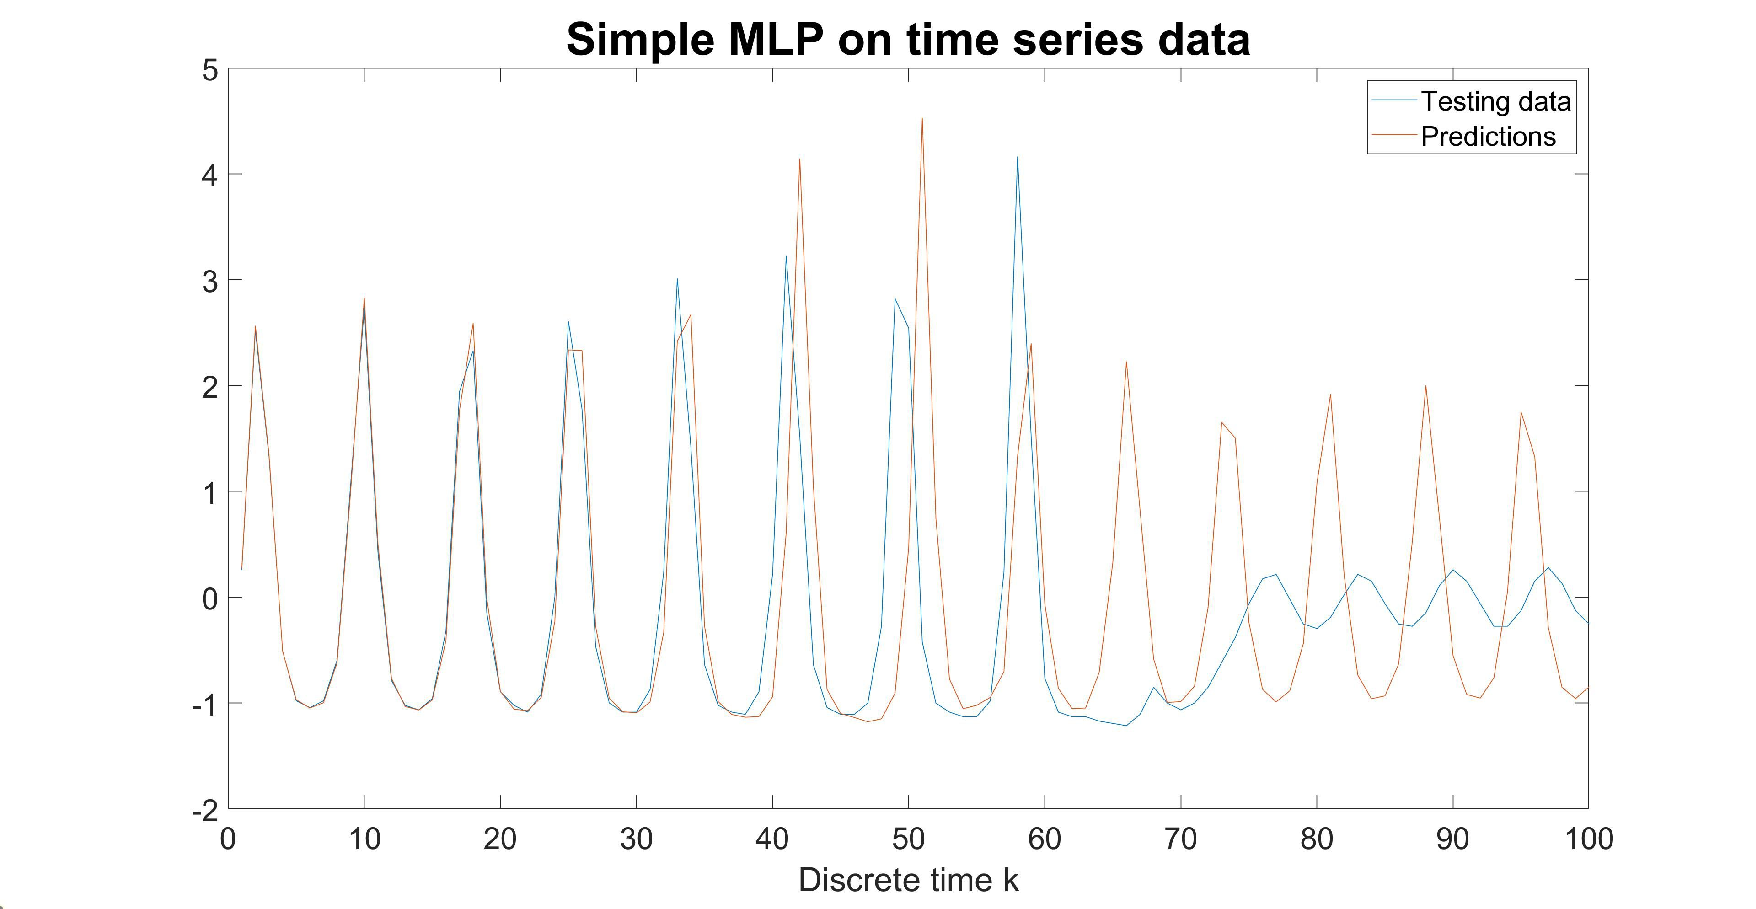
\includegraphics[width=\linewidth]{lab2/mlp_avg.pdf}
  \caption{MLP with one hidden layer on time series (avg)}
  \label{fig:mlpavg}
\end{subfigure}
\hfill
\begin{subfigure}[b]{.49\textwidth}
  \centering
  % include first image
  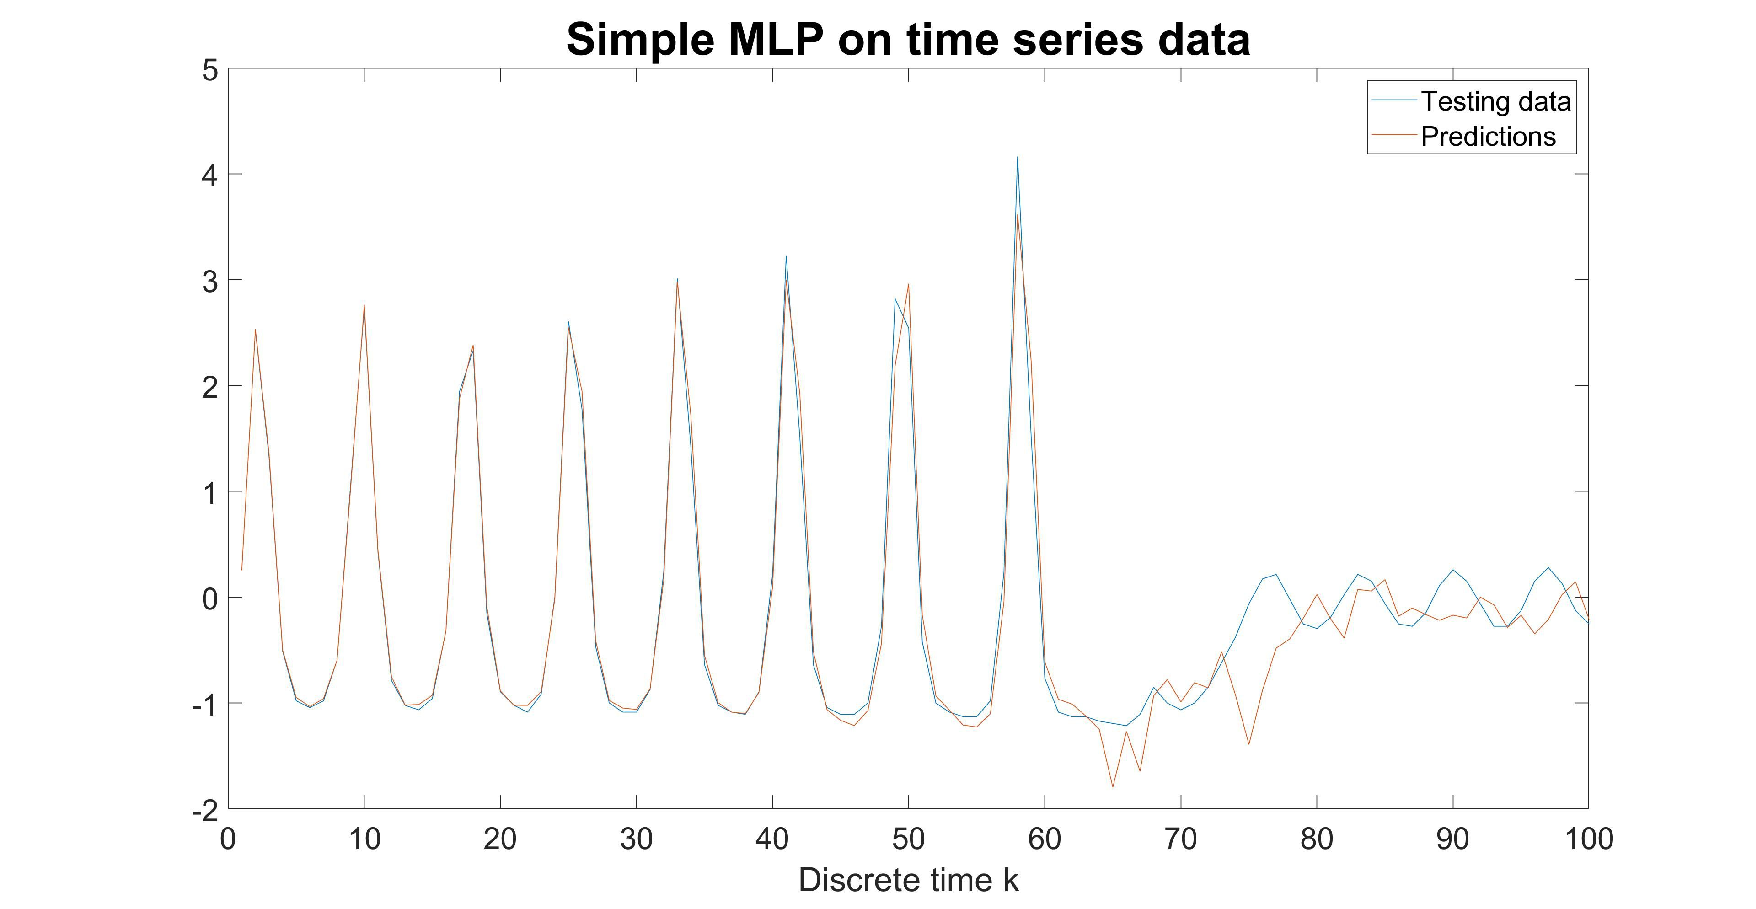
\includegraphics[width=\linewidth]{lab2/mlp.pdf}
  \caption{MLP with one hidden layer on time series (best)}
  \label{fig:nlpbest}
\end{subfigure}
\caption{MLP with one hidden layer on time series}
\label{fig:mlp}
\end{figure}

\subsection{LSTM}

LSTM is a unique structured recurrent neural network. It has these specially designed gates which enable it to choose what to forget and what to remember, this gives LSTM the ability to act much more similar to a human brain on memory processing.

Here we used the template code provided by MATLAB official documentation\footnote{Time Series Forecasting Using Deep Learning, https://nl.mathworks.com/help/deeplearning/ug/time-series-forecasting-using-deep-learning.html}. There are a few parameters that we could tune to adjust the performance of LSTM: number of hidden units (neurons), training solver (algorithm), epoch numbers, gradient threshold, initial learning rate, when and what dropped learning rate, and the lag value for the dataset. 

In our case, we try to adopt a very simple LSTM as the documentation used. We used \verb|adam| as our backbone solver as it is usually more optimised than gradient descent in the field of deep learning. However, it requires more computational power than the traditional \verb|trainlm| and \verb|traingd| we used before. Here we set the training parameters as:

\begin{verbatim}
numFeatures = 1;
numResponses = 1;
numHiddenUnits = 80;

layers = [ ...
    sequenceInputLayer(numFeatures)
    lstmLayer(numHiddenUnits)
    fullyConnectedLayer(numResponses)
    regressionLayer];

options = trainingOptions('adam', ...
    'MaxEpochs',800, ...
    'GradientThreshold',1, ...
    'InitialLearnRate',0.005, ...
    'LearnRateSchedule','piecewise', ...
    'LearnRateDropPeriod',160, ...
    'LearnRateDropFactor',0.5, ...
    'Verbose',0, ...
    'Plots','training-progress');
\end{verbatim}

Here we specified the initial learn rate 0.005 (same in the sample code), and drop the learning rate after 160 epochs (1/5 of overall 800 epochs) by multiplying by a factor of 0.5. In general, we usually drop the learning rate after 20\% to 30\% of the entire dataset, and we do not want the learning rate to drop too much. Learning rate is a significant value for training neural networks; it determines how quickly a model adapts to the dataset. Usually, a small learning rate needs more epochs to train as there are not enough weight change every update cycle. However, a high learning rate may cause the model to converge too quickly to a suboptimal solution, whereas a learning rate that is too small can cause the process to get stuck.

For hidden neurons, we have tested several numbers vary from 10 to 100 and stuck with 80 as it gave us the best result. We were noted that the RMSE could be reduced less than 100 even with a small hidden neuron numbers like 40. Here, aiming to the best result, we, however, used 80. Figure \ref{fig:lstmfinal} shows the training process of our LSTM network and Figure \ref{fig:lstmresult} gives the prediction result on testing dataset.

\begin{figure}[h!]
  \centering
  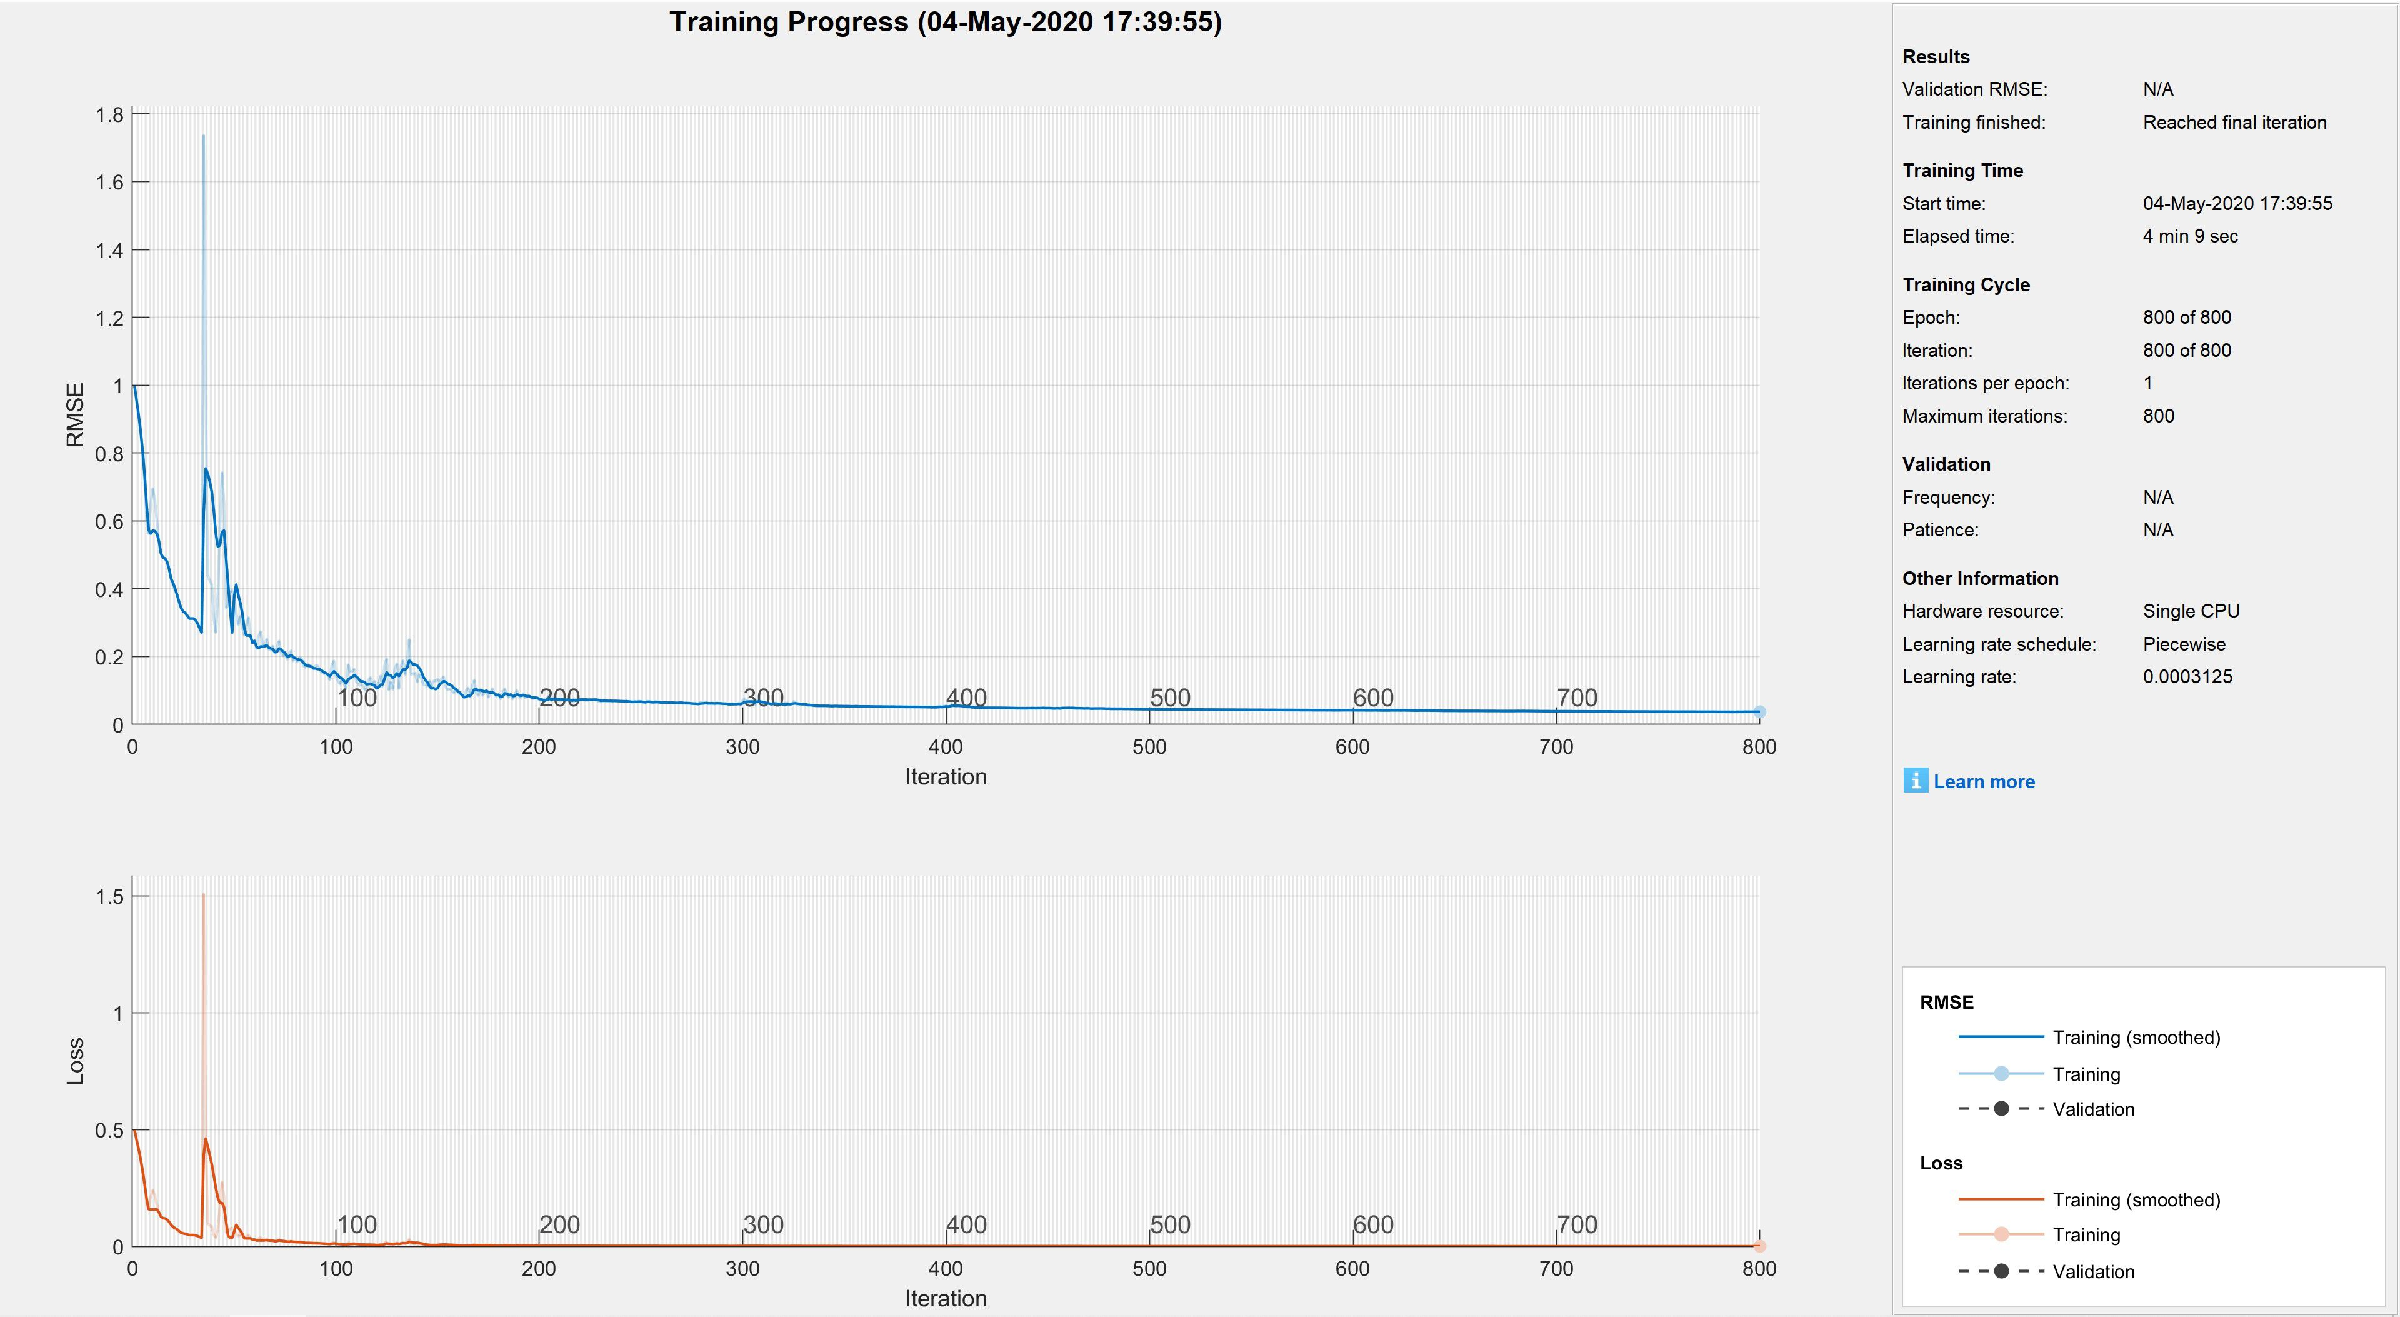
\includegraphics[width=\textwidth]{lab2/lstmfinal.pdf}
  \caption{LSTM training process with best settings}
  \label{fig:lstmfinal}
\end{figure}

\begin{figure}[h!]
  \centering
  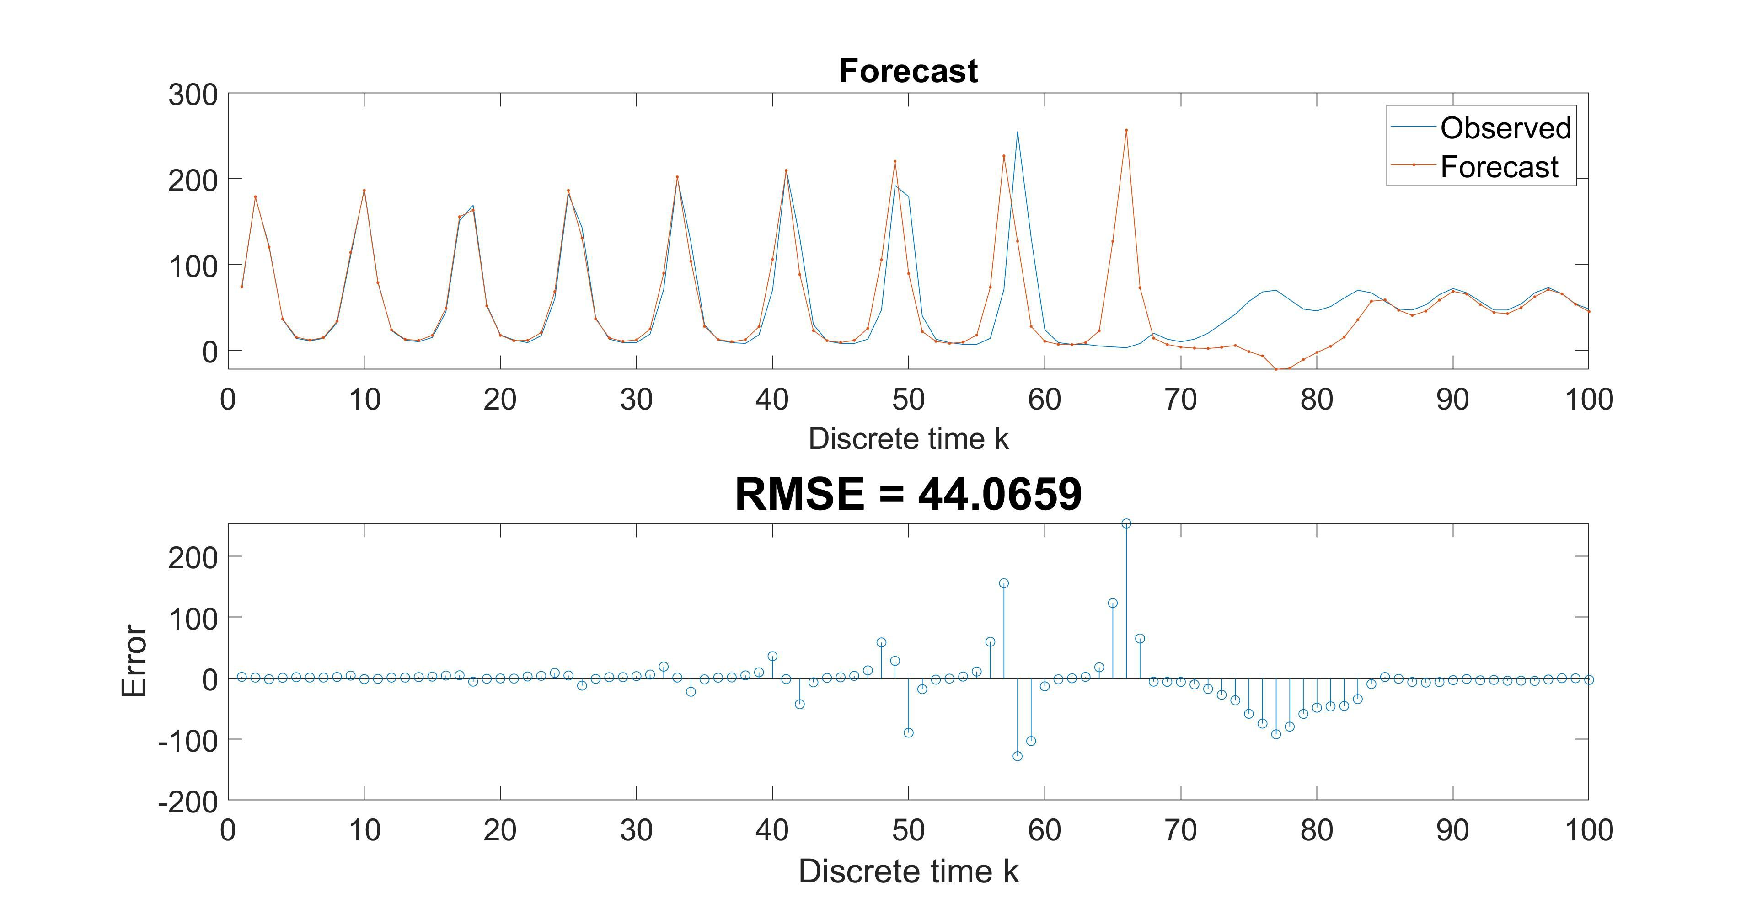
\includegraphics[width=\textwidth]{lab2/lstmresult.pdf}
  \caption{Result of LSTM}
  \label{fig:lstmresult}
\end{figure}

We have already known that significant drift happens around the $60^{th}$ point of testing set; this requires much longer knowledge from the past for our neural network to determine. The significant difference between na\"ive MLP and LSTM is the ability to recognise and memorise the dependencies between those data points, which significantly helped LSTM to capture and predict the significant drift in the testing set.

Until now, we used the previous prediction as input to the function for each prediction. Furthermore, as we now have access to the actual values of time steps between predictions, then we can update the network state with the observed values instead of the predicted values. Figure \ref{fig:lstmimprovedresult} compared the forecasted values with the test data, and we noticed a significant improvement on prediction accuracy when updating the network state with the observed values instead of the predicted values.

\begin{figure}[h!]
  \centering
  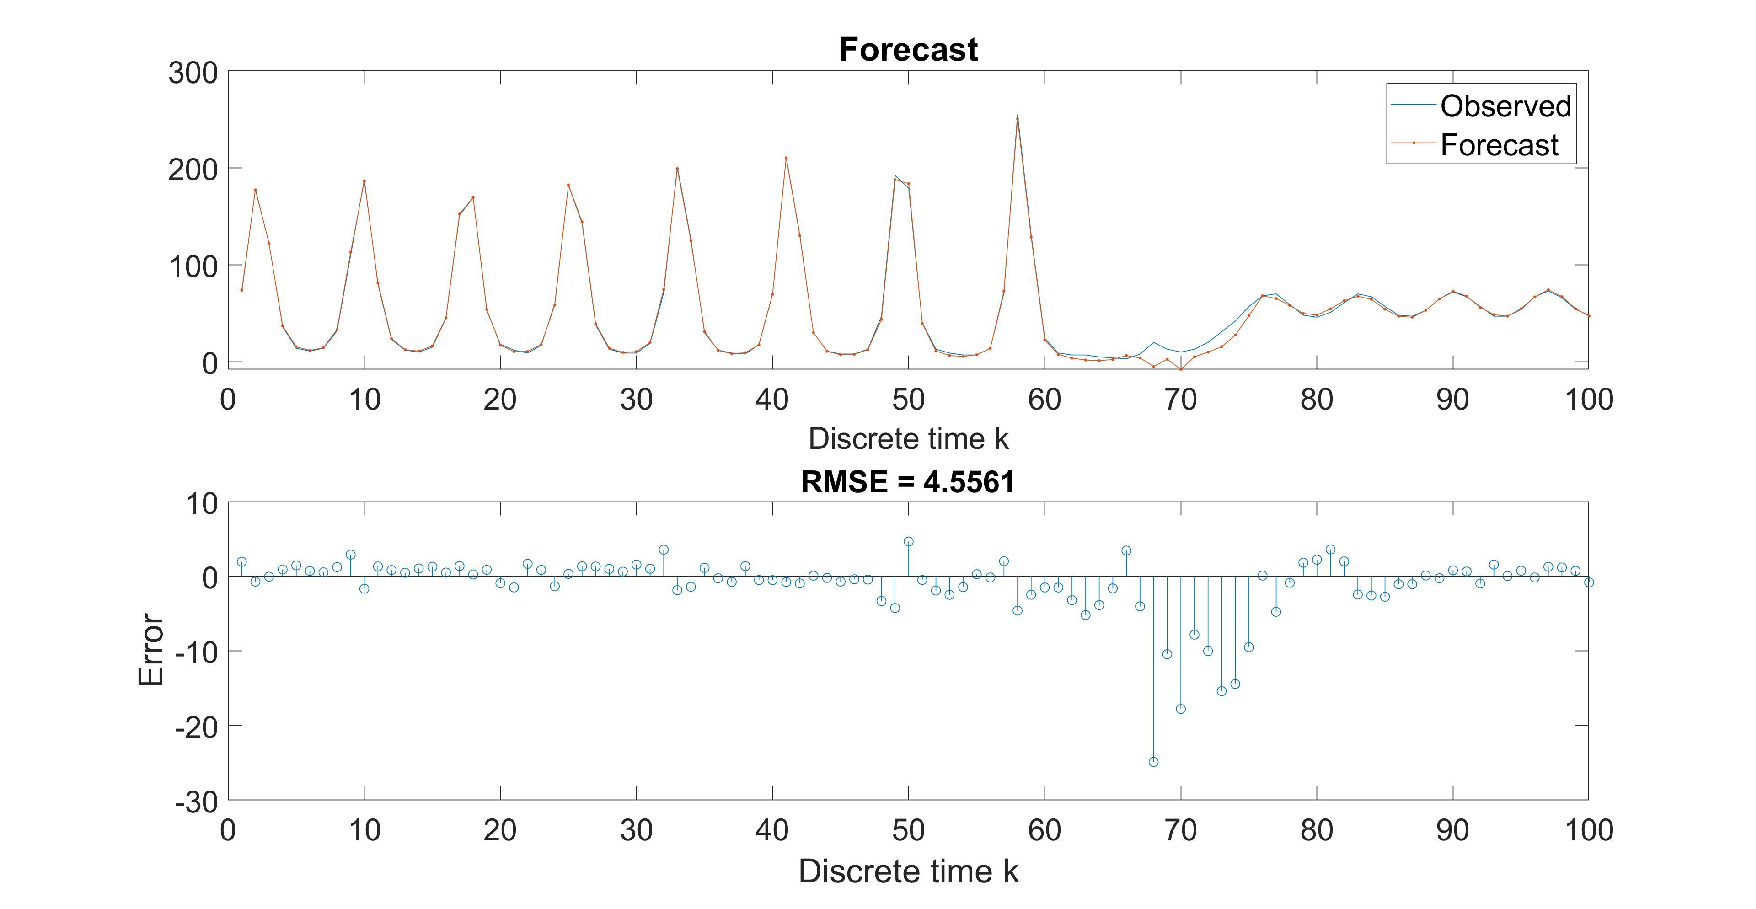
\includegraphics[width=\textwidth]{lab2/lstmimproved.pdf}
  \caption{Result of improved LSTM}
  \label{fig:lstmimprovedresult}
\end{figure}


\section{Deep feature learning}

\subsection{Principal Component Analysis}

We first compare the root mean square difference between the reconstructed (Using PCA) and the original data (Gaussian random numbers and \verb|choles_all|(highly correlated)). Result is shown in Figure \ref{fig:pca1}.

\begin{figure}[h!]
\begin{subfigure}[b]{.49\textwidth}
  \centering
  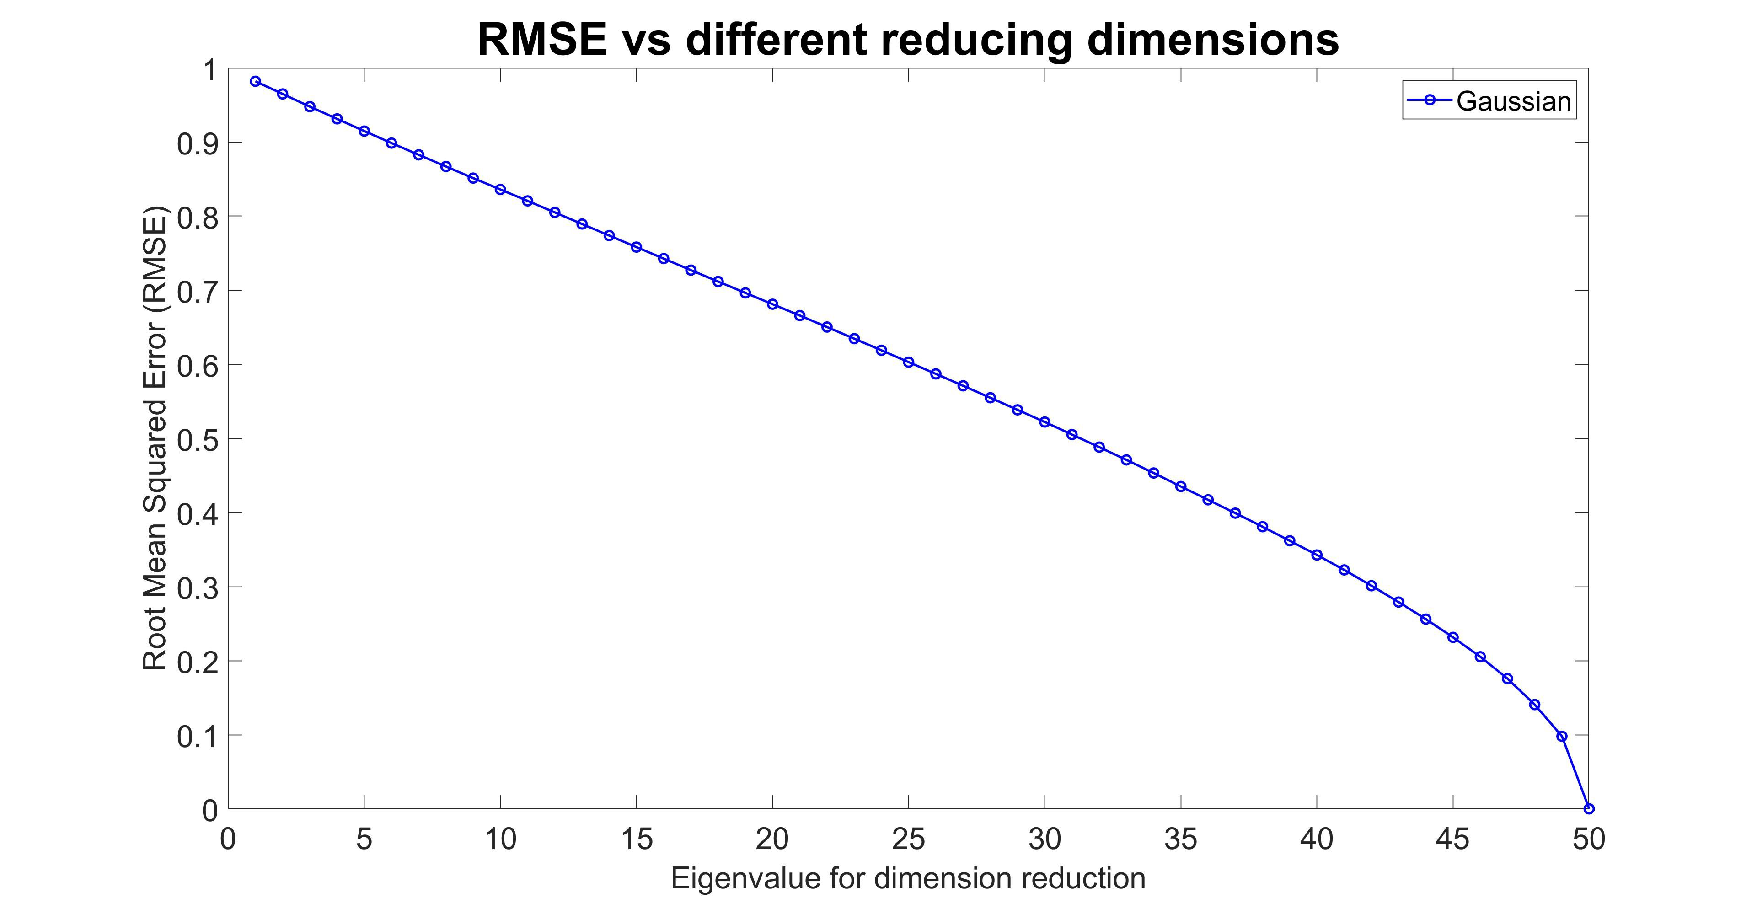
\includegraphics[width=\linewidth]{lab3/gaussianrmse.pdf}
  \caption{RMSE vs eigenvalues (Gaussian random)}
  \label{fig:pcaGaussian}
\end{subfigure}
\hfill
\begin{subfigure}[b]{.49\textwidth}
  \centering
  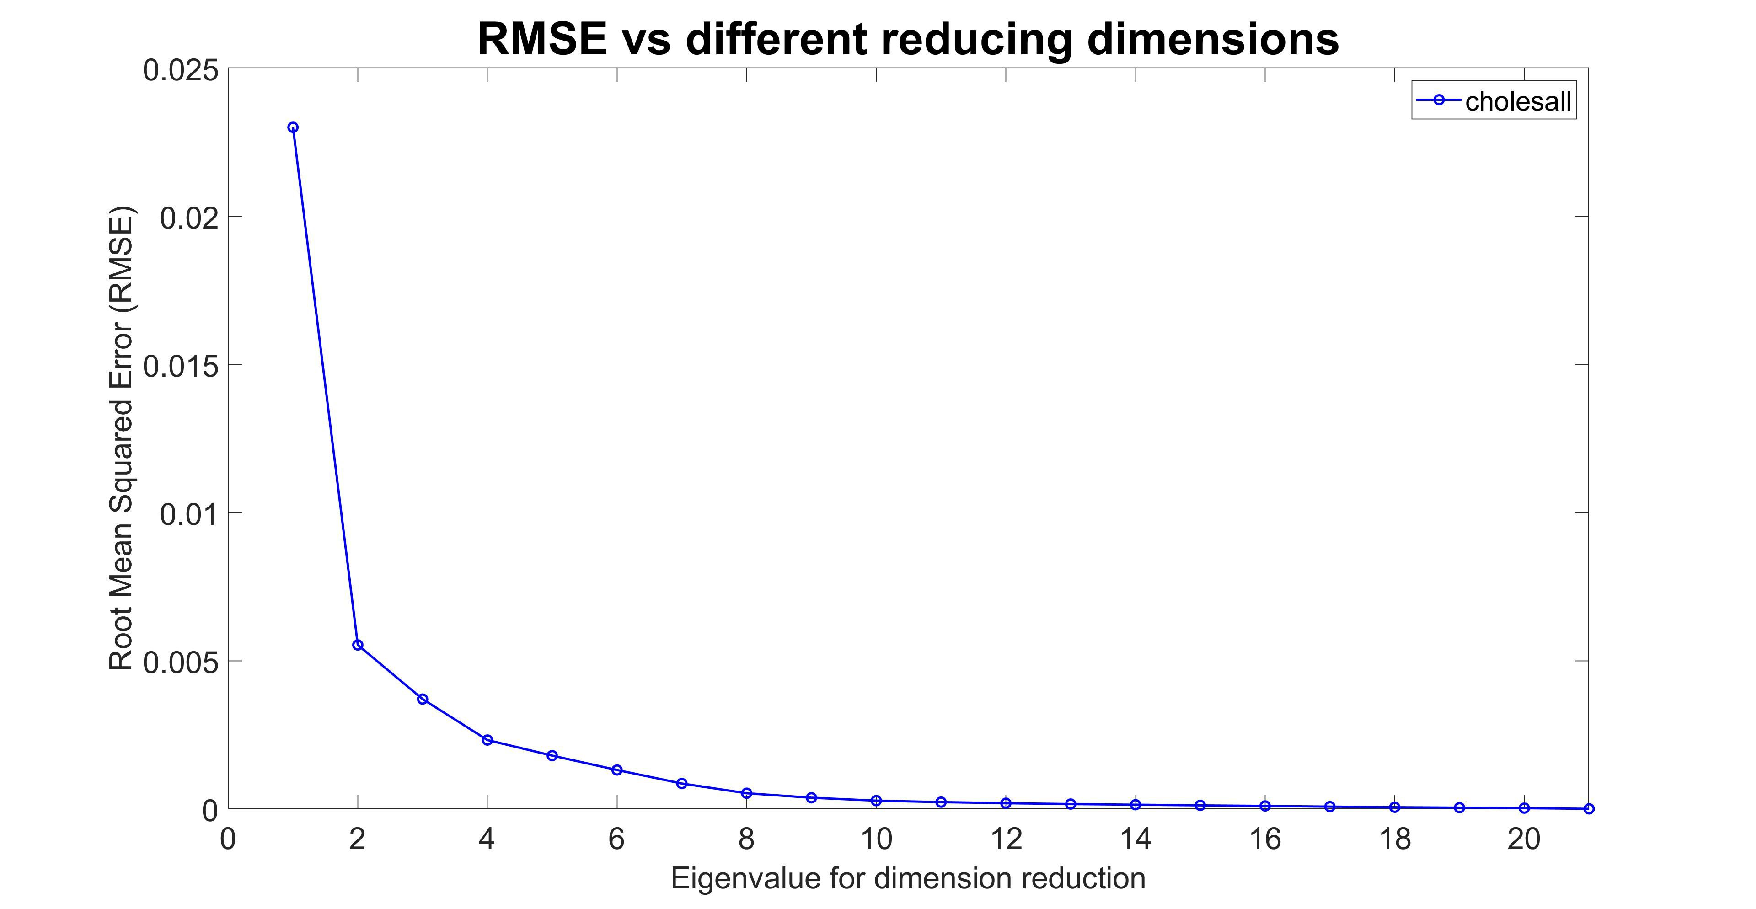
\includegraphics[width=\linewidth]{lab3/choles.pdf}
  \caption{RMSE vs eigenvalues (highly correlated)}
  \label{fig:pcacholes}
\end{subfigure}
\caption{RMSE vs eigenvalues}
\label{fig:pca1}
\end{figure}

Next section focuses on ``performing PCA on handwritten images of the digit 3 taken from the US Postal Service database''. Firstly, we show the mean ``3'' below as in Figure \ref{fig:mean3} along with the eigenvalues of the covariance matrix of the input digit data.

\begin{figure}[h!]
  \centering
  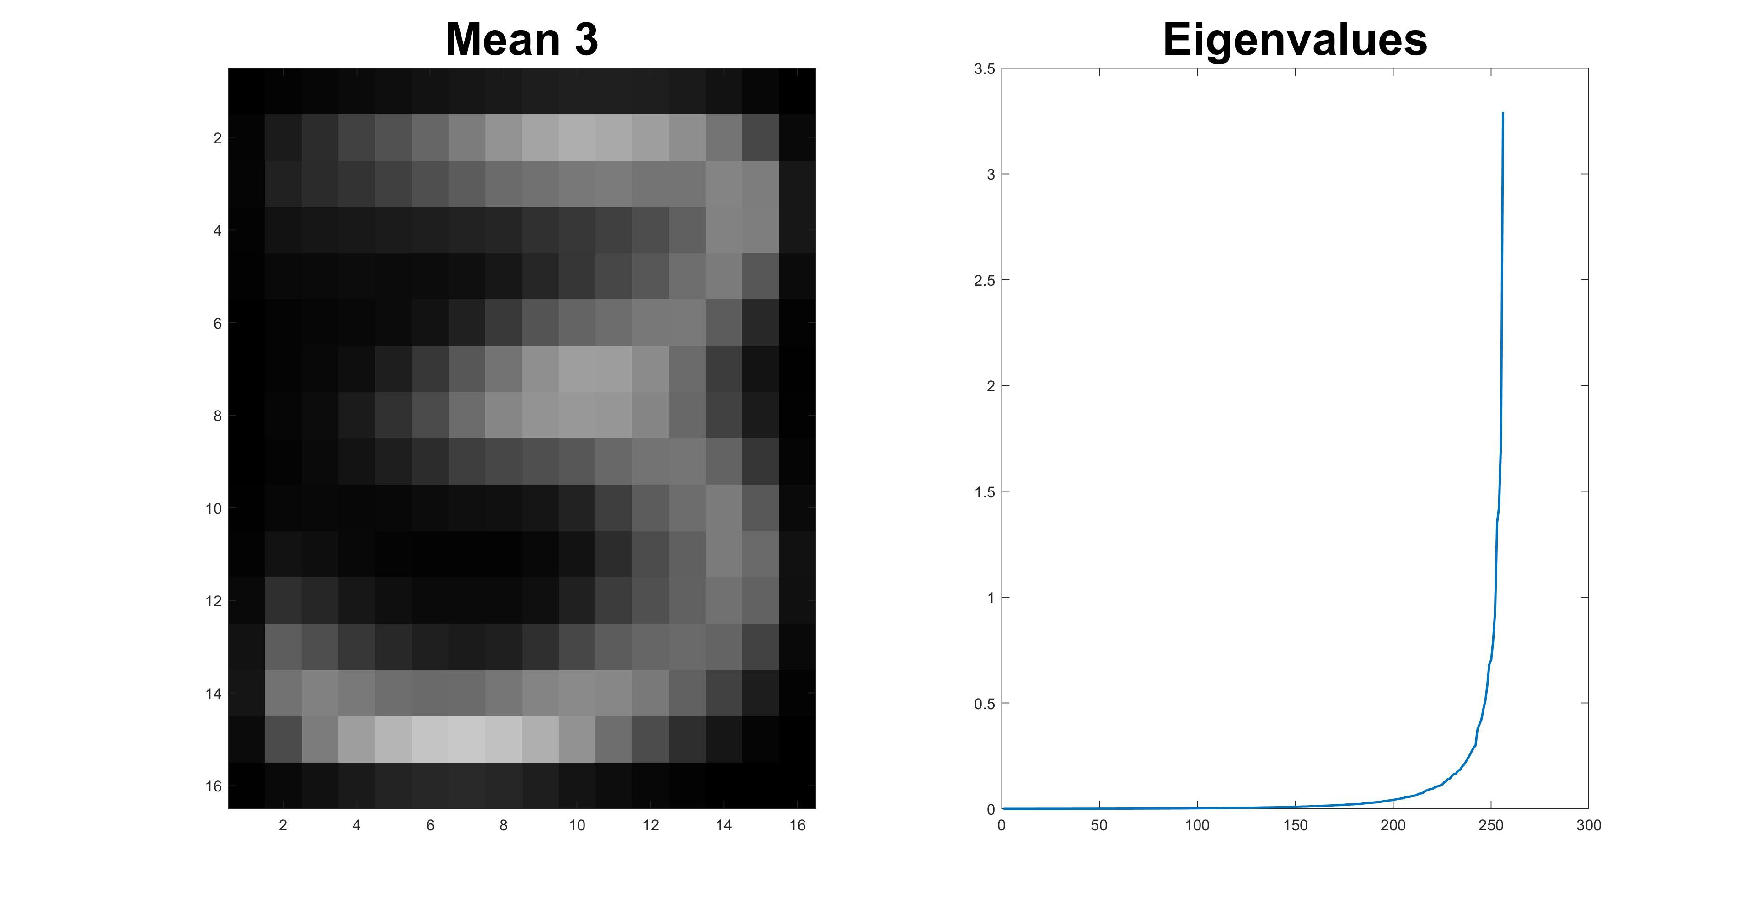
\includegraphics[width=\textwidth]{lab3/mean3eigenvalues.pdf}
  \caption{mean of digit ``3''}
  \label{fig:mean3}
\end{figure}

Now as told, we ``compress the dataset by projecting it onto one, two, three, and four principal components. Now reconstruct the images
from these compressions and plot some pictures of the four reconstructions.'' The reconstructed ``3'' are shown in Figure \ref{fig:3indiffq} along with the original one and more various values of eigenvalues. It is interesting to notice that even with such a small eigenvalue like $q=1$, we can still use fresh eyes to recognise the digit. After $q$ reaches around 100, the reconstructed digit is very close to the original one.

\begin{figure}[h!]
  \centering
  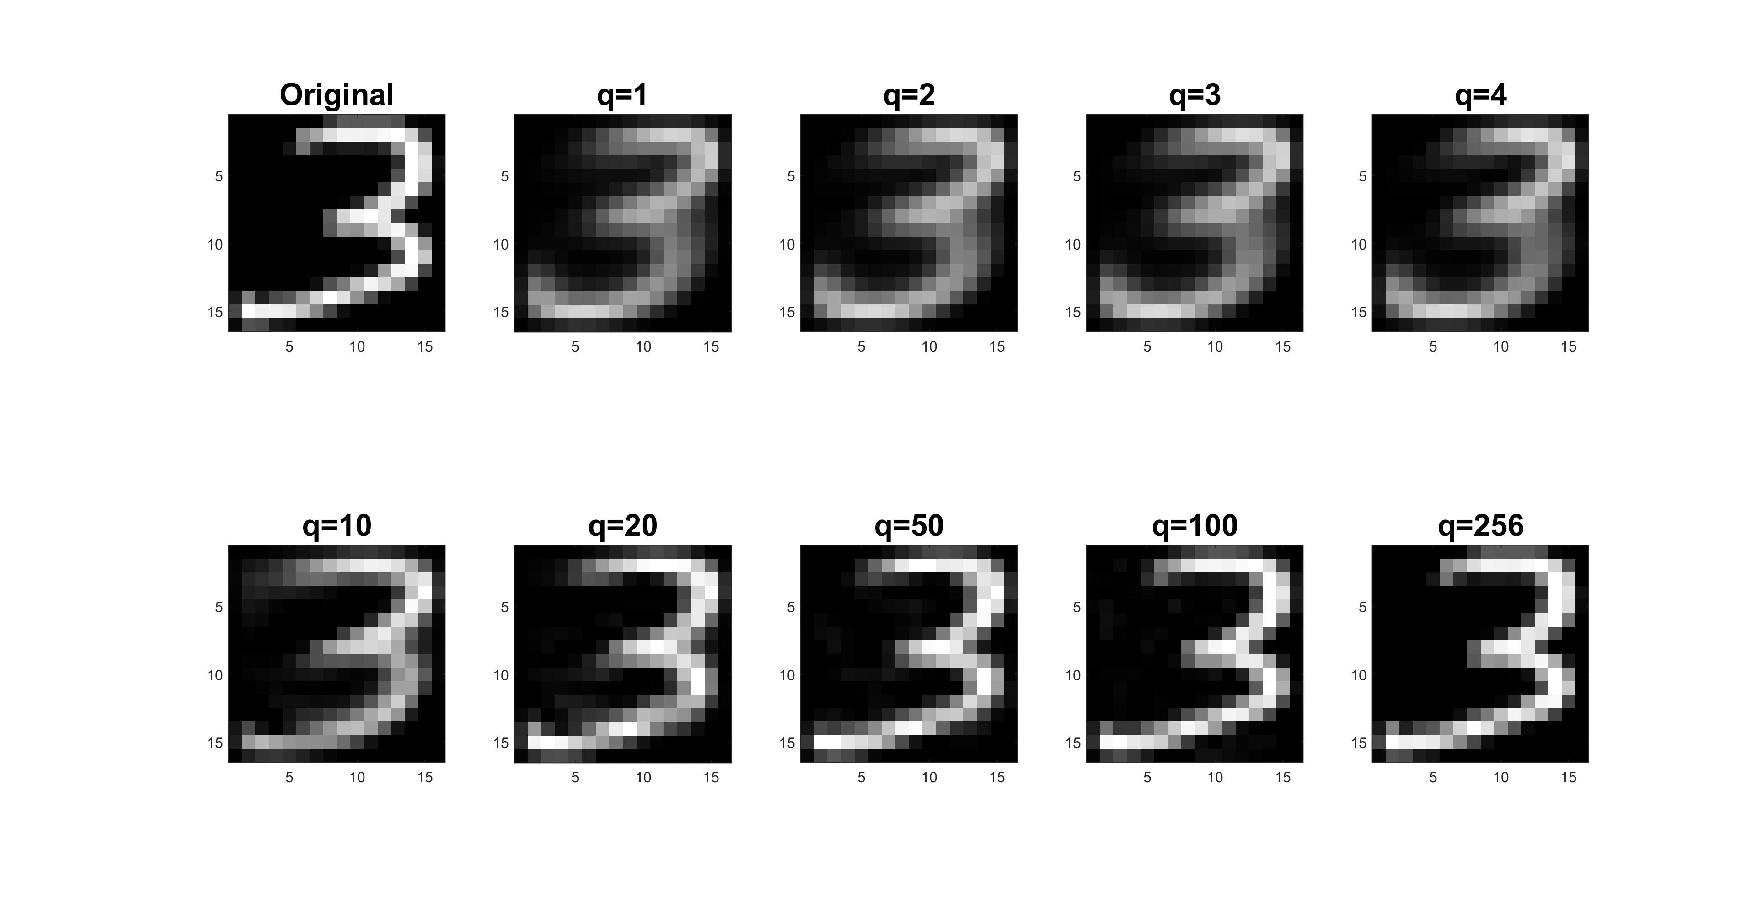
\includegraphics[width=\textwidth]{lab3/3indiffq.pdf}
  \caption{Digit ``3'' in different eigenvalues (q)}
  \label{fig:3indiffq}
\end{figure}

Figure \ref{fig:msevsq} illustrates the error curve by different eigenvalues $q$. We can answer the question of MSE when $q=256$ with the figure.

\begin{figure}[h!]
  \centering
  \includegraphics[width=\textwidth]{lab3/msevsq.pdf}
  \caption{MSE vs eigenvalues ($\protect q$)}
  \label{fig:msevsq}
\end{figure}

\subsection{Stacked Autoencoders}
The power of the deep network lies in its ability to learn multiple representations of the original data layer by layer. The bottom layer provides basic expression which is learnt by succeeding layers. Deep learning is more capable for solving complex classification problems.

The stacked autoencoder does the same as above. As mentioned, a single autoencoder can learn a feature change $h = f\theta(x)$ through a three-layer network of fictitious $x\Rightarrow h\Rightarrow x$ (here $\theta$ represents the transformed parameters, including $W$, $b$ and activation function). We have obtained the feature expression $h$, so can we use $h$ as the original information and train a new autoencoder to get a new feature expression? This is called Stacked Autoencoder (SAE).

Here we test different parameters ``(\verb|MaxEpochs|, number of hidden neurons in each layer, number of layers) and to compare the performance of the stacked autoencoder to a normal multilayer
neural network'', in this case, non-deep standard neural network. In order to get a more accurate experimental result, we aim to get multiple runs for each experimental settings then vary those parameters. However, considering the CPU only training processing requires a massive amount of time, we only run each combination of parameters three times. For \verb|MaxEpochs| of the autoencoder, we test {400, 200, 50} epochs for the first hidden layer, then succeeding layer will have half of the epoch numbers. For neurons in the hidden layer, we set them in the final layer as {20, 100}, and each preceding hidden layer will have double neurons. 

Here to simplify the experiments, we used only tested on deep network using one or two autoencoders. 

\begin{table}[h!]
\begin{tabular}{lcc}
\hline \hline
                      & \multicolumn{1}{l}{\begin{tabular}[c]{@{}l@{}}Testing accuracy(2-layer SAE)\\ Fine-tuned (mean, max)\end{tabular}} & \multicolumn{1}{l}{\begin{tabular}[c]{@{}l@{}}Testing accuracy(2-layer SAE)\\ (mean, max)\end{tabular}} \\ \hline
epoch=400, neuron=100 & (99.7320, 100)                                                                                                     & (85.0720, 86.0210)                                                                                      \\ \hline
epoch=400, neuron=20  & (99.1730, 99.5230)                                                                                                 & (84.7150, 85.3920)                                                                                      \\ \hline
epoch=200, neuron=100 & (99.5480, 99.8420)                                                                                                 & (84.8210, 85.4280)                                                                                      \\ \hline
epoch=50, neuron=20   & (98.9200, 99.3450)                                                                                                 & (83.9290, 85.0300)                                                                                      \\ \hline\hline
                      & \multicolumn{1}{l}{\begin{tabular}[c]{@{}l@{}}Testing accuracy (2-layer NN)\\ (mean, max)\end{tabular}}       & \multicolumn{1}{l}{\begin{tabular}[c]{@{}l@{}}Testing accuracy (single-layer NN)\\ (mean, max)\end{tabular}} \\ \hline
epoch=400, neuron=100 & (95.7880, 97.2830)                                                                                                 & (96.1480, 97.5840)                                                                                      \\ \hline
epoch=400, neuron=20  & (94.9800, 97.0720)                                                                                                 & (94.9230, 96.8340)                                                                                      \\ \hline
epoch=200, neuron=100 & (95.0330, 97.1900)                                                                                                 & (95.5210, 96.9250)                                                                                      \\ \hline
epoch=50, neuron=20   & (94.5820, 96.2450)                                                                                                 & (94.0720, 96.4570)                                                                                      \\ \hline
\end{tabular}
\caption{Testing accuracy on different networks (two autoencoder)}
\label{tab:sae}
\end{table}

Table \ref{tab:sae} illustrates some experimental result from our testing process. It is interesting to see that without fine-tuning, the SAE would become very vulnerable and cannot even surpass the simplest MLP. Once an SAE works with fine-tuned, the result significantly increased and with enough epoch and neurons, it can even each 100\% in some runs, even a very simple autoencoder with only 20 neurons and running 50 epochs, the fine-tuned result is still auspicious - 96\% on average. 

It is also curious that the number of epoch does not affect the result much, but an increased number of neurons does make some changes. However, when we increased numbers of hidden layers (i.e. one more autoencoder in the deep network), this significantly improved the deep network. Generally speaking, two autoencoders perform better than single but only with proper fine-tuning. Fine-tuning is exceptionally crucial when there are more than one autoencoders and not enough neurons in each layer because the output of each encoder have already captured enough well-represented features of the input. 

While each new autoencoder tries to reconstruct the activations of the previous autoencoder's hidden layer, however, the last autoencoder (that will be the last layer of our multilayer autoencoder during fine-tuning) is different, this one will use the activations of the previous layer and tries to reconstruct the 'global' input (i.e. the original input that was fed to the first layer). This process is often referred to as fine-tuning or simply another back-propagation. 

Overall, more neurons in each layer and two autoencoders can achieve a good result in this case. Fine-tuning is the key for multiple autoencoders to generate good result. Also noted, for simple MLP, it is often sufficient enough to use just one single layer instead of more layers as they will more possibly cause overfitting - having very high training accuracy but not so satisfactory testing accuracy.

\subsection{CNN}

\subsubsection{Questions in 3.2}

\begin{itemize}

    \item Q: Take a look at the first convolutional layer (layer 2) and at the dimension of the weights, what do these weights represent?
    \item A: Figure \ref{fig:1stconvo} shows the weights in the first convolutional layer. We know that the input images are in the size of $(227\times227)$ with three colour channels: red, green and blue. Our first convolutional layer has 96 convolution masks of the size of $(11\times11\times3)$ with $[4\;4]$ sized stride and padding $[0\;0\;0\;0]$. After passing through this convolutional layer, the image becomes abstracted to a feature map, with shape $(55\times55\times96)$, (feature map width $\times$ feature map height $\times$ feature map channels). In this layer, for every pixel, after the  96 masking with $[4\;4]$ stride, this should result with 96 output with average height and width $(227-11)/4+1=55$.
    \item Q: Inspect layers 1 to 5. If you know that a ReLU and a Cross Channel Normalisation layer do not affect the dimension of the input, what is the dimension of the input at the start of layer 6 and why?
    \item A: We know layer 1 is input layer with $(227\times227\times3)$, layer 2 is convolutional layer with $(55\times55\times3)$ output. Layer 3 and 4 do not change dimensions; however, layer 5 does $(3\times3)$ max pooling with $[2\;2]$ sized stride and padding $[0\;0\;0\;0]$. So the output dimension of layer 5 or the input size of layer 6 (second convolutional layer) should be $(55/2+1)=27\times27\times96$.
    \item Q: What is the dimension of the inputs before the final classification part of the network (i.e. before the fully connected layers)? How does this compare with the initial dimension? Briefly discuss the advantage of CNNs over fully connected networks for image classification.
    \item A: The last fully connected layer has the dimension of 1,000 - there are 1,000 neurons for the final classification task. However, only 3 of them are being used to predict the classes: aeroplane, ferry or laptop. Comparing to the initial dimension which is $(227\times227\times3)=154,587$, dimension is significantly reduced. Generally speaking, CNN is very effective on image classification as the concept of dimension reduction suits the huge number of parameters in an image.
\end{itemize}


\begin{figure}[h!]
\begin{subfigure}[b]{.49\textwidth}
  \centering
  \includegraphics[width=.15\linewidth]{lab3/alexnet.pdf}
  \caption{AlexNet architecture}
  \label{fig:alexnet}
\end{subfigure}
\hfill
\begin{subfigure}[b]{.49\textwidth}
  \centering
  \includegraphics[width=\linewidth]{lab3/1stclayer.pdf}
  \caption{1st convolutional layer weights}
  \label{fig:1stconvo}
\end{subfigure}
\caption{RMSE vs eigenvalues}
\label{fig:fig}
\end{figure}
\subsubsection{Digit classification with CNN}

In this section, we ran some CNN architectures on the handwritten digits dataset used before on SAE. There are some parameters we experimented: numbers of layers, various combinations of different kinds of layers, dimensions of the weights, etc.

First, there are some parameters in training we want to test under the provided sample combination of layers. The starting settings for training are listed below:

\begin{verbatim}
options = trainingOptions('sgdm', ...
    'LearnRateSchedule','piecewise', ...
    'LearnRateDropFactor',0.2, ...
    'LearnRateDropPeriod',5, ...
    'MaxEpochs',20, ...
    'MiniBatchSize',128, ...
    'InitialLearnRate',0.0001,'OutputFcn',@plotTrainingAccuracy);
\end{verbatim}

\paragraph{Solver}
There are three major training solvers: \verb|sgdm| (stochastic gradient descent with momentum (SGDM) optimiser), \verb|rmsprop| (RMSProp optimiser), and \verb|adam| (Adam optimiser). We tested both \verb|sgdm| and \verb|adam| solvers on some settings and noticed very subtle difference on the performance, so we went with \verb|adam| for all the next tunings processes.

\paragraph{\# of epoch and mini-batch size}
\verb|MaxEpochs| here stands for the maximum number of epochs to use for training. An iteration is one step taken in the gradient descent algorithm towards minimising the loss function using a mini-batch. An epoch represents a complete round of finishing the training process over the entire training dataset. And regarding \verb|MiniBatchSize|, generally, it may influence the convergence of our optimisation algorithm (\verb|sgdm| or \verb|adam|), and how much memory is used during the computation. Note that it is generally preferred now to use smaller batch sizes (4, 16, 32, 64, 128), considering we only have 1,000 images per digit. 

After tested different \verb|MiniBatchSize| with different \verb|MaxEpochs|, we can conclude that small mini-batch size as 4 or 16 can achieve impeccable results with almost any \verb|MaxEpochs| (in this case: 10, 50, 100). Smaller  \verb|MiniBatchSize| converge faster and achieve a better result by enabling more GD steps, larger \verb|MaxEpochs| can help improve the accuracy but the impact is minimal.

\paragraph{Learning rate}

Learning rate has always been the most important hyper-parameter in the neural network training process. Instead of using a constant learning rate, we choose to make it adaptive by decay the learning rate every couple epochs. This is done by tuning the parameters \verb|InitialLearnRate|, \verb|LearnRateDropFactor|, \verb|LearnRateDropPeriod|.

We have used various combination of learning rate related parameters. We usually start our learning rate from $10^{-2}$ to $10^{-5}$. According to Deep Learning book: ``\textit{In practice, it is necessary to gradually decrease the learning rate over time, so we now denote the learning rate at iteration. This is because the SGD gradient estimator introduces a source of noise (the random sampling of m training examples) that does not vanish even when we arrive at a minimum.}'' \footnote{Deep Learning, An MIT Press book, by Ian Goodfellow and Yoshua Bengio and Aaron Courville} So here we found out that starting from 0.001 and decay 0.5 every 10 batches in overall 100 batches could produce an excellent result: 99.23\% accuracy.

\paragraph{Network architecture}

After discussed enough on the training parameter tuning, we move to the architecture of our neural network. There are choices between using different numbers of convolutional layers, different filter size, and varying amounts of filter/neurons/feature maps. We have known that more convolutional layers usually benefit the accuracy result as each convolutional layer reduces the number of input features to the fully connected layers, although after about two or three layers the accuracy gain becomes rather small. So here we stick with two convolutional layers to save computational power. Meanwhile, the accuracy was guaranteed. 

As there is no magic formula for deciding upon the number of filter/neurons in each convolutional layer, it is applicable and beneficial to start with an excessive amount of nodes, then to remove the unnecessary nodes through pruning. We found out that with the original settings, we were able to obtain a perfect accuracy 99.87\%, which is more than satisfactory, so we chose to keep the default settings.

\paragraph{Best settings}

\begin{verbatim}
options = trainingOptions('adam', ...
    'LearnRateSchedule','piecewise', ...
    'LearnRateDropFactor',0.5, ...
    'LearnRateDropPeriod',10, ...
    'MaxEpochs',100, ...
    'MiniBatchSize',4, ...
    'InitialLearnRate',0.001,'OutputFcn',@plotTrainingAccuracy);
    
layers = [imageInputLayer([28 28 1])
    convolution2dLayer(5,12)
    reluLayer
    maxPooling2dLayer(2,'Stride',2)
    convolution2dLayer(5,24)
    reluLayer  
    fullyConnectedLayer(10)
    softmaxLayer
    classificationLayer()];
\end{verbatim}

\section{Generative models}

\subsection{RBM}
The two layers of a restricted Boltzmann machine (RBM) are called the hidden or output layer and the visible or input layer. The various nodes across both the layers are connected. But, in each of the layers, there is no connection between any two nodes belonging to the same layer.

It is really hard to pick a useful guidance metrics for picking optimal hyper-parameters to train RBM, because we are not able to estimate the log-likelihood $log p(v)$ directly during training (with partition function $Z$).\footnote{Hinton, G. E. (2002). Training products of experts by minimizing contrastive divergence. Neural Computation, 14(8):1711–1800.}

%%%%%%
\begin{figure}[h!]
     \centering
     %%%
     \begin{subfigure}[b]{0.3\textwidth}
         \centering
         \includegraphics[width=\textwidth]{lab4/test.pdf}
         \caption{Testing set}
         \label{fig:noise5ite10}
     \end{subfigure}
     \hfill
     \begin{subfigure}[b]{0.3\textwidth}
         \centering
         \includegraphics[width=\textwidth]{lab4/100_0.01_20_5.pdf}
         \caption{N=100, lr=0.01, ite=20, gibbs=5}
         \label{fig:noise5ite100}
     \end{subfigure}
     \hfill
     \begin{subfigure}[b]{0.3\textwidth}
         \centering
         \includegraphics[width=\textwidth]{lab4/100_0.01_20_500.pdf}
         \caption{N=100, lr=0.01, ite=20, gibbs=500}
         \label{fig:noise5ite500}
     \end{subfigure}
     %%%
     \begin{subfigure}[b]{0.3\textwidth}
         \centering
         \includegraphics[width=\textwidth]{lab4/200_0.001_20_5.pdf}
         \caption{N=200, lr=0.001, ite=20, gibbs=5}
         \label{fig:noise5ite10}
     \end{subfigure}
     \hfill
     \begin{subfigure}[b]{0.3\textwidth}
         \centering
         \includegraphics[width=\textwidth]{lab4/200_0.001_20_500.pdf}
         \caption{N=200, lr=0.001, ite=20, gibbs=500}
         \label{fig:noise5ite100}
     \end{subfigure}
     \hfill
     \begin{subfigure}[b]{0.3\textwidth}
         \centering
         \includegraphics[width=\textwidth]{lab4/1000_0.001_20_10.pdf}
         \caption{N=1000, lr=0.001, ite=20, gibbs=10}
         \label{fig:noise5ite500}
     \end{subfigure}
    %%%
     \begin{subfigure}[b]{0.3\textwidth}
         \centering
         \includegraphics[width=\textwidth]{lab4/100_0.01_20_1_0-10.pdf}
         \caption{N=100, lr=0.01, ite=20, gibbs=1, (0-10)}
         \label{fig:noise10ite10}
     \end{subfigure}
     \hfill
     \begin{subfigure}[b]{0.3\textwidth}
         \centering
         \includegraphics[width=\textwidth]{lab4/100_0.01_20_1_0-15.pdf}
         \caption{N=100, lr=0.01, ite=20, gibbs=1, (0-15)}
         \label{fig:noise10ite100}
     \end{subfigure}
     \hfill
     \begin{subfigure}[b]{0.3\textwidth}
         \centering
         \includegraphics[width=\textwidth]{lab4/100_0.01_20_1_0-20.pdf}
         \caption{N=100, lr=0.01, ite=20, gibbs=1, (0-20)}
         \label{fig:noise10ite500}
     \end{subfigure}
     %%%
     \begin{subfigure}[b]{0.3\textwidth}
         \centering
         \includegraphics[width=\textwidth]{lab4/50_0.01_20_10_10-20.pdf}
         \caption{N=50, lr=0.01, ite=20, gibbs=10, (10-20)}
         \label{fig:noise10ite10}
     \end{subfigure}
     \hfill
     \begin{subfigure}[b]{0.3\textwidth}
         \centering
         \includegraphics[width=\textwidth]{lab4/200_0.001_20_10_0-15.pdf}
         \caption{N=200, lr=0.001, ite=20, gibbs=10, (0-15)}
         \label{fig:noise10ite100}
     \end{subfigure}
     \hfill
     \begin{subfigure}[b]{0.3\textwidth}
         \centering
         \includegraphics[width=\textwidth]{lab4/1000_0.001_20_10_0-15.pdf}
         \caption{N=1000, lr=0.001, ite=20, gibbs=10, (0-15)}
         \label{fig:noise10ite500}
     \end{subfigure}
     
        \caption{RBM}
        \label{fig:rbm}
\end{figure}

%%%%%%%
\subsubsection{Number of Gibbs steps}
Theoretically speaking, RBM can obtain a better learning result if there are more Gibbs sampling steps used - we get better approximations of gradient. However, this did not reflect on our experiments on MNIST, which shows actually only one alternating Gibbs sampling can help getting good learning results - more Gibbs sampling steps may decrease the quality of filters and samples.

%%%%%%%%
\subsubsection{Learning rate}
From the discussed before, we know that learning rate cannot be too large which may explode the weights and dramatically increase the reconstruction error, it cannot be too small either - slows down the learning process a lot. We should keep it in the interval between [0.0001, 0.01]. 

\begin{figure}[h!]
     \centering
     %%%
     \begin{subfigure}[b]{0.3\textwidth}
         \centering
         \includegraphics[width=\textwidth]{lab4/1000_0.001_20_10.pdf}
         \caption{N=1000, lr=0.001, ite=20, gibbs=10}
         \label{fig:noise5ite10}
     \end{subfigure}
     \hfill
     \begin{subfigure}[b]{0.3\textwidth}
         \centering
         \includegraphics[width=\textwidth]{lab4/1000_0.001_20_5_0-15.pdf}
         \caption{N=1000, lr=0.001, ite=20, gibbs=5, (0-15)}
         \label{fig:noise5ite100}
     \end{subfigure}
     \hfill
     \begin{subfigure}[b]{0.3\textwidth}
         \centering
         \includegraphics[width=\textwidth]{lab4/1000_0.001_20_100_0-15.pdf}
         \caption{N=1000, lr=0.001, ite=20, gibbs=100, (0-15)}
         \label{fig:noise5ite500}
     \end{subfigure}
        \caption{Noise=10}
        \label{fig:hopnoise10}
\end{figure}

%%%%%%%%
\subsubsection{Number of hidden units}

In most cases we choose to use more hidden units than visible ones to handle more information processing tasks. However, in the field of discriminative learning, ``the amount of constraints imposed on parameters by the training case is equal to the number of bits spent on the specified label'', labels usually have very limited information which means more hidden units may easily cause severe overfitting that is extremely dangerous. Nevertheless, when generative models are adopted to learn high-dimensional data, it should be fair to fit a very large number of parameters to training images. 

To avoid overfitting and try to save computational power, we tested on 50, 100 and 200 neurons (all small numbers). It clearly showed that more hidden neurons help getting better results.

\subsubsection{Number of missing rows}
We tested on missing different numbers of rows from top to bottom of a digit image. After increased the number of removed rows to 15, the reconstruction started to struggle. With right numbers of hyperparameter settings, missing 15 rows can still be fairly reconstructed.

\subsubsection{Filters}
The filters learnt by the model can be visualised, the first 100 filters extracted by RBM is shown as Figure \ref{fig:first100rbm}. The figure plots weights of each hidden unit as a gray-scale image. Every filter should be able to pick out clear features from the dataset. While it is not clear for an arbitrary dataset, in this case, for MNIST dataset, it works more like stroke detectors.

\begin{figure}[h!]
  \centering
  \includegraphics[width=.4\textwidth]{lab4/rbmfinal100.pdf}
  \caption{First 100 filters extracted by RBM}
  \label{fig:first100rbm}
\end{figure}
\subsection{DBM}
Different from A RBM, which is a Boltzmann machine whose nodes must be a bipartite graph, a DBM is simply a deep Boltzmann machine.

Figure \ref{fig:bmarchi}\footnote{Wang, Haohan \& Raj, Bhiksha. (2017). On the Origin of Deep Learning.} gives us an idea on the difference of BM, RBM and DBM. Simply speaking, RBM is a BM with restrictions (no connection within hidden or visible nodes), DBM is a stacked version RBM. Figure \ref{fig:traindbm} illustrates the training process of DBM.

With greedy layer by layer pretraining structure, DBM has the ability to speed up the weight learning process. This process uses contrasting divergence to learn stacked RBM.

How this greedy layer by layer training works in DBM? To compensate the insufficient top-down input for the first hidden layer and, we double the input of the lower level RBM inside a DBM. And to compensate the insufficient bottom-up input we double the hidden neurons for top most level RBM. For those layers in between, their RBM weights are also doubled.

Figure \ref{fig:dbmsample} shows the result samples generated by DBM with different numbers of Gibbs sampling. We notice that the result is better than RBM. Now adding various hidden layers like in DBM, can help the network to come up with relations even from the deepest layers and thus the input can be more finely understood by the network which will help it learn a better model.

\begin{figure}[h!]
\begin{subfigure}[b]{.49\textwidth}
  \centering
  \includegraphics[width=\linewidth]{lab4/bmgraph.pdf}
  \caption{Boltzmann machine architecture}
  \label{fig:bm}
\end{subfigure}
\hfill
\begin{subfigure}[b]{.49\textwidth}
  \centering
  \includegraphics[width=\linewidth]{lab4/rbmgraph.pdf}
  \caption{RBM layer weights}
  \label{fig:rbm}
\end{subfigure}
%%%
\begin{subfigure}[b]{.49\textwidth}
  \centering
  \includegraphics[width=\linewidth]{lab4/dbmgraph.pdf}
  \caption{DBM architecture}
  \label{fig:dbm}
\end{subfigure}
\hfill
\begin{subfigure}[b]{.49\textwidth}
  \centering
  \includegraphics[width=\linewidth]{lab4/dbm.pdf}
  \caption{Process of training DBM network}
  \label{fig:traindbm}
\end{subfigure}
\caption{Boltzmann machines (Wang et al. (2017))}
\label{fig:bmarchi}
\end{figure}

\begin{figure}[h!]
\begin{subfigure}[b]{.49\textwidth}
  \centering
  \includegraphics[width=.6\linewidth]{lab4/dbmfinal1.pdf}
  \caption{1st layer of DBM}
  \label{fig:1stdbm}
\end{subfigure}
\hfill
\begin{subfigure}[b]{.49\textwidth}
  \centering
  \includegraphics[width=.6\linewidth]{lab4/dbmfinal2.pdf}
  \caption{2nd layer of DBM}
  \label{fig:2nddbm}
\end{subfigure}
\caption{DBM layers}
\label{fig:dbmlayers}
\end{figure}

\begin{figure}[h!]
     \centering
     %%%
     \begin{subfigure}[b]{0.3\textwidth}
         \centering
         \includegraphics[width=.9\textwidth]{lab4/dbmgibb1.pdf}
         \caption{Samples generated by DBM (1 Gibbs)}
         \label{fig:dbm1gibb}
     \end{subfigure}
     \hfill
     \begin{subfigure}[b]{0.3\textwidth}
         \centering
         \includegraphics[width=.9\textwidth]{lab4/dbm100gibb.pdf}
         \caption{Samples generated by DBM (100 Gibbs)}
         \label{fig:dbm100gibb}
     \end{subfigure}
     \hfill
     \begin{subfigure}[b]{0.3\textwidth}
         \centering
         \includegraphics[width=.9\textwidth]{lab4/dbmgibb5000.pdf}
         \caption{Samples generated by DBM (5000 Gibbs)}
         \label{fig:dbm5000gibb}
     \end{subfigure}
        \caption{Samples generated by DBM}
        \label{fig:dbmsample}
\end{figure}

\subsection{Generative Adversarial Networks (GAN)}
Generative Adversarial Networks consists of two neural networks:
\begin{itemize}
    \item A discriminator $D$ is a discriminating network, discriminating whether an image is ``real''. Its input parameter is $x$, $x$ represents an image, the output $D(x)$ represents the probability that $x$ is a real image, if it is 1, it means 100\% is a real image, and the output is 0, it means that it cannot be a true image.
    \item A generator $G$ is a network that generates images. It receives a random noise $z$, and generates images through this noise, denoted as $G(z)$.
\end{itemize}

In the training process, the goal of generating network $G$ is to generate as real image as possible to deceive and discriminate network $D$. The goal of $D$ is to separate the images generated by G from the real images as much as possible. In this way, $G$ and $D$ constitute a dynamic ``game process''.

What is the result of the final game? In the most ideal state, $G$ can generate a image $G(z)$ that is sufficiently fool $D$. For D, it is difficult to determine whether the image generated by $G$ is real or not, so $D(G(z)) = 0.5$.

$$
\min _{G} \max _{D} V(D, G)=\mathbb{E}_{\boldsymbol{x} \sim p_{\text {data }}(\boldsymbol{x})}[\log D(\boldsymbol{x})]+\mathbb{E}_{\boldsymbol{z} \sim p_{\boldsymbol{z}}(\boldsymbol{z})}[\log (1-D(G(\boldsymbol{z})))]
$$

Simply analyse the formula above:
\begin{itemize}
    \item The whole formula consists of two items. $x$ represents the real image, $z$ represents the noise input to the $G$ network, and $G(z)$ represents the image generated by the $G$ network.
    \item $D(x)$ represents the probability that the $D$ network judges whether an image is real (because $x$ is real, so for D, the closer this value is to 1, the better). $D(G(z))$ is the probability that the $D$ network judges whether the image generated by $G$ is real.
    \item The purpose of $G$: As mentioned above, $D(G(z))$ is the probability that the $D$ network judges whether the image generated by $G$ is real. $G$ should hope that the image generated by itself is ``the closer to the real, the better.'' In other words, $G$ wants $D(G(z))$ to be as large as possible, and then $V(D, G)$ will become smaller. So we see that the first sign of the formula is $min_G$.
    \item Purpose of $D$: The stronger the ability of $D$, the bigger $D(x)$ should be, and the smaller $D(G(x))$ should be. At this time $V(D, G)$ will become larger. Therefore, the formula aims for a maximum $D$.
\end{itemize}

Figure \ref{fig:ganresult} demonstrates the ``class 1'' image generated by GAN from the CIFAR dataset with different numbers of epochs (20k and 50k), there is a visible image quality improvement from 20k to 50k epochs. Also, from the training process we noticed that the loss and accuracy of the generator vs discriminator are constantly changing without a visible pattern. GAN has been known with several weakness which we will discuss in the following paragraphs.

\begin{figure}[h!]
     \centering
     %%%
     \begin{subfigure}[b]{0.49\textwidth}
         \centering
         \includegraphics[width=.9\textwidth]{lab4/Class1 20000epochs 32batch.pdf}
         \caption{GAN result (class 1 with 20k epochs)}
         \label{fig:gan20k}
     \end{subfigure}
     \hfill
     \begin{subfigure}[b]{0.49\textwidth}
         \centering
         \includegraphics[width=.9\textwidth]{lab4/Class1 50000epochs 32batch.pdf}
         \caption{GAN result (class 1 with 50k epochs)}
         \label{fig:gan50k}
     \end{subfigure}
        \caption{GAN result}
        \label{fig:ganresult}
\end{figure}


\subsubsection{Weakness of GAN}
Although GAN has shown great success in the realistic image generation, the training is not easy; The process is known to be slow and unstable. \footnote{Salimans et al. (2016). Improved techniques for training GAN. (NIPS’16)} We noticed that the loss and accuracy for $G$ and $D$ in our experiments kept changing and cannot remain stable or achieve a final convergence.

\paragraph{No convergence guaranteed}
The basic problem currently facing is: all theories believe that GAN should have excellent performance in Nash equilibrium, but gradient descent can only guarantee the realisation of Nash equilibrium in the case of convex function. When both sides of the game ($G$ and $D$) are represented by a neural network, it is possible to keep them always adjusting their strategies without actually reaching equilibrium.

\paragraph{Hard to control}
Compared with other generative models, the competitive approach of GAN no longer requires a hypothetical data distribution, that is, it does not need to formulate $p(x)$, but uses a distribution to directly sample, so that it can be very close to the real data theoretically , which is also the biggest advantage of GAN.

However, the disadvantage of GAN is there is n pre-modeling required - it has too much freedom. For larger images and those have more pixels, the simple GAN-based method is less controllable. In GAN, every time the learning parameter update process is set to $D$ update $k$ times while $G$ only updates one time, is also designed for similar considerations.

\paragraph{Difficult to train: collapse problem}
The GAN model is defined as a minimum and maximum problem with no loss function, and it is difficult to distinguish whether progress is being made during the training process. 

A collapse problem may occur in the learning process of GAN. The generator starts to degenerate, always generating the same sample points, and unable to continue learning. When the generated model ($G$) collapses, the discriminant model ($D$) will point in similar directions to similar sample points, and training cannot continue.

\subsection{Optimal transport}

Different from directly move pixels to transfer colours, optimal transport use Wasserstein metric to calculate the optimum distance between two colour distributions.

Here the goal is to move colour from a given configuration to a desired configuration in the minimum cost or minimum distance. However, besides Wasserstein, we also have Kullback-Leibler (KL) divergence, that is widely mentioned in machine learning and statistics for similar uses.

The original GAN under the optimised discriminator, minimising the loss of the generator is equivalent to Jensen–Shannon divergence that minimises the distribution generated by the generator and the target distribution. But using JS divergence as a measure has a fatal flaw, that is, in the case where the two distributions do not intersect each other, the JS divergence of the two distributions will always be constant $\mathrm{log}_2$. And because the distribution generated by the generator and the target distribution support set are low-dimensional manifolds embedded in the high-dimensional space, the measure of their overlapping part is almost zero.

This makes it impossible to measure the distance between two distributions without intersection. When calculating the gradient, there will also be a zero gradient. Since both JS divergence and KL divergence have problems with the above measurements, this distance measurement method is not continuous and derivable everywhere. But our GAN needs a derivable and continuous measurement method. Using optimal transport divergence as a measurement method can solve the above problems of JS divergence and KL divergence.

The first step consists in defining the source and target sets $X$, $Y$, which involves spatio-colour clustering on the input images $u$, $v$, respectively. These clusters are then used to build a weighted graph $\left(\omega_{i, j}\right)$ and define the transport cost matrix $C_{XY}$ that are involved in the local adaptive functional to minimise. The colour transfer is finally applied using the estimated regularised transport map (Wasserstein).

Here we also tested different levels of regularisations, with more regularisation levels, the finial adaption result will have more global effects which means some irrelevant regions are also get colour transferred.

\begin{figure}[h!]
     \centering
     %%%
     \begin{subfigure}[b]{0.3\textwidth}
         \centering
         \includegraphics[width=\textwidth]{lab4/ot0.01-min.pdf}
         \caption{OT (reg=0.01)}
         \label{fig:ot0.01}
     \end{subfigure}
     \hfill
     \begin{subfigure}[b]{0.3\textwidth}
         \centering
         \includegraphics[width=\textwidth]{lab4/ot0.1-min.pdf}
         \caption{OT (reg=0.1)}
         \label{fig:ot0.1}
     \end{subfigure}
     \hfill
     \begin{subfigure}[b]{0.3\textwidth}
         \centering
         \includegraphics[width=\textwidth]{lab4/ot0.5-min.pdf}
         \caption{OT (reg=0.5)}
         \label{fig:ot0.5}
     \end{subfigure}
        \caption{Optimal transport for colour transport}
        \label{fig:ot}
\end{figure}

\subsection{WGAN}

Like we discussed above in Optimal Transport, Wasserstein Distance is a measure of the distance between two probability distributions. 

While JS or KL divergence are both popular using as loss function in GAN, Wasserstein became the right choice to solve the problem of training instability of GAN. The KL divergence and JS divergence are abrupt, either the largest or the smallest, but the Wasserstein distance is smooth. If we use the gradient descent method to optimise the distance parameter, the first two cannot provide the gradient at all, but the Wasserstein distance can. Similarly, in a high-dimensional space, if the two distributions do not overlap or the overlap is negligible, KL and JS can neither reflect the distance nor provide the gradient, but Wasserstein can provide a meaningful gradient.

WGAN introduces Wasserstein distance. Because of its superior smoothness relative to KL divergence and JS divergence, it can theoretically solve the problem of gradient disappearance. Then the Wasserstein distance is written into a solvable form through a mathematical transformation. Using a discriminator neural network with limited parameter value ranges to maximise this form, the Wasserstein distance can be approximated. Under this approximate optimal discriminator, the optimised generator makes the Wasserstein distance narrow, which can effectively narrow the generated distribution and the real distribution. WGAN not only solves the problem of unstable training, but also provides a reliable training process indicator, and this indicator is indeed highly related to the quality of the generated samples.

From the result shown below in Figure \ref{fig:3wgan}, it is obvious that WGAN and WGAN with weight clipping clearly surpassed the standard GAN. The generated disgits were much better represented with clear shapes.

\begin{figure}[h!]
     \centering
     %%%
     \begin{subfigure}[b]{0.3\textwidth}
         \centering
         \includegraphics[width=\textwidth]{lab4/wgan1.pdf}
         \caption{Wasserstein GAN}
         \label{fig:wgan}
     \end{subfigure}
     \hfill
     \begin{subfigure}[b]{0.3\textwidth}
         \centering
         \includegraphics[width=\textwidth]{lab4/wgan2.pdf}
         \caption{Standard GAN}
         \label{fig:gan}
     \end{subfigure}
     \hfill
     \begin{subfigure}[b]{0.3\textwidth}
         \centering
         \includegraphics[width=\textwidth]{lab4/wgan3.pdf}
         \caption{WGAN with Weight Clipping}
         \label{fig:wganwc}
     \end{subfigure}
        \caption{Wasserstein GAN}
        \label{fig:3wgan}
\end{figure}

\end{document}
